%%%%%%%%%%%%%%%%%%%%%%%%%%%%%%%%%%%%%%%%%
% Masters/Doctoral Thesis 
% LaTeX Template
% Version 2.3 (25/3/16)
%
% This template has been downloaded from:
% http://www.LaTeXTemplates.com
%
% Version 2.x major modifications by:
% Vel (vel@latextemplates.com)
%
% This template is based on a template by:
% Steve Gunn (http://users.ecs.soton.ac.uk/srg/softwaretools/document/templates/)
% Sunil Patel (http://www.sunilpatel.co.uk/thesis-template/)
%
% Template license:
% CC BY-NC-SA 3.0 (http://creativecommons.org/licenses/by-nc-sa/3.0/)
%
%%%%%%%%%%%%%%%%%%%%%%%%%%%%%%%%%%%%%%%%%

%----------------------------------------------------------------------------------------
%	PACKAGES AND OTHER DOCUMENT CONFIGURATIONS
%----------------------------------------------------------------------------------------

\documentclass[
11pt, % The default document font size, options: 10pt, 11pt, 12pt
%oneside, % Two side (alternating margins) for binding by default, uncomment to switch to one side
%chapterinoneline,% Have the chapter title next to the number in one single line
%english, % ngerman for German
spanish,
singlespacing, % Single line spacing, alternatives: onehalfspacing or doublespacing
%draft, % Uncomment to enable draft mode (no pictures, no links, overfull hboxes indicated)
%nolistspacing, % If the document is onehalfspacing or doublespacing, uncomment this to set spacing in lists to single
%liststotoc, % Uncomment to add the list of figures/tables/etc to the table of contents
%toctotoc, % Uncomment to add the main table of contents to the table of contents
parskip, % Uncomment to add space between paragraphs
%nohyperref, % Uncomment to not load the hyperref package
headsepline, % Uncomment to get a line under the header
]{MastersDoctoralThesis} % The class file specifying the document structure



\usepackage[utf8]{inputenc} % Required for inputting international characters
\usepackage[T1]{fontenc} % Output font encoding for international characters

\usepackage{palatino} % Use the Palatino font by default
%,style=authoryear
\usepackage[backend=bibtex,natbib=true]{biblatex} % Use the bibtex backend with the authoryear citation style (which resembles APA)

\addbibresource{references.bib} % The filename of the bibliography

\usepackage[autostyle=true]{csquotes} % Required to generate language-dependent quotes in the bibliography

\usepackage{caption}
\usepackage{subcaption}

%------------------------
\usepackage{listings}

%\usepackage[hyphens]{url}
%\usepackage[hidelinks]{hyperref}
%\hypersetup{breaklinks=true}
\urlstyle{same}
%\usepackage{cite}

%--------------------------

\usepackage{color}

%
%----------------------------------------------------------------------------------------
%	MARGIN SETTINGS
%----------------------------------------------------------------------------------------

\geometry{
	paper=a4paper, % Change to letterpaper for US letter
	inner=2cm, % Inner margin
	outer=3.3cm, % Outer margin
	bindingoffset=2cm, % Binding offset
	top=1.5cm, % Top margin
	bottom=1.5cm, % Bottom margin
	%showframe,% show how the type block is set on the page
}

%----------------------------------------------------------------------------------------
%	INFORMACIÓN DE LA MEMORIA
%----------------------------------------------------------------------------------------

\thesistitle{CIAABOT: Robótica educativa abierta sobre CIAA} % El títulos de la memoria, se usa en la carátula y se puede usar el cualquier lugar del documento con el comando \ttitle
\supervisor{Ing. Eric Pernía} % El nombre del director, se usa en la carátula y se puede usar el cualquier lugar del documento con el comando \supname
\degree{Especialista en Sistemas Embebidos } % Nombre del grado, se usa en la carátula y se puede usar el cualquier lugar del documento con el comando \degreename
\author{Ing. Leandro Lanzieri Rodríguez} % Tu nombre, se usa en la carátula y se puede usar el cualquier lugar del documento con el comando \authorname
\juradoUNO{Dr. Ing. Pablo Gómez (FIUBA)} % Nombre y pertenencia del un jurado se usa en la carátula y se puede usar el cualquier lugar del documento con el comando \jur1name
\juradoDOS{Esp. Ing. Ernesto Gigliotti (UTN FRA)} % Nombre y pertenencia del un jurado se usa en la carátula y se puede usar el cualquier lugar del documento con el comando \jur2name
\juradoTRES{Esp. Ing. Patricio Bos (FIUBA)} % Nombre y pertenencia del un jurado se usa en la carátula y se puede usar el cualquier lugar del documento con el comando \jur3name
\fechaINICIO{febrero de 2017}
\fechaFINAL{diciembre de 2017}

\subject{Memoria del Trabajo Final de la Carrera de Especialización en Sistemas Embebidos de la UBA} % Your subject area, this is not currently used anywhere in the template, print it elsewhere with \subjectname
\keywords{CESE, Sistemas Embebidos, CIAA} % Keywords for your thesis, this is not currently used anywhere in the template, print it elsewhere with \keywordnames
\university{Universidad de Buenos Aires} % Your university's name and URL, this is used in the title page and abstract, print it elsewhere with \univname
\faculty{{Facultad de Ingeniería}} % Your faculty's name and URL, this is used in the title page and abstract, print it elsewhere with \facname
\department{Departamento de Electrónica} % Your department's name and URL, this is used in the title page and abstract, print it elsewhere with \deptname
\group{{Laboratorio de Sistemas Embebidos}} % Your research group's name and URL, this is used in the title page, print it elsewhere with \groupname


\hypersetup{pdftitle=\ttitle} % Set the PDF's title to your title
\hypersetup{pdfauthor=\authorname} % Set the PDF's author to your name
\hypersetup{pdfkeywords=\keywordnames} % Set the PDF's keywords to your keywords


\newcaptionname{spanish}{\acknowledgementname}{Agradecimientos}
\newcaptionname{spanish}{\authorshipname}{Declaración de Autoría}
\newcaptionname{spanish}{\abbrevname}{Glosario}
\newcaptionname{spanish}{\byname}{por}

\renewcommand{\lstlistingname}{Algoritmo}% Listing -> Algorithm
\renewcommand{\lstlistlistingname}{Índice de \lstlistingname s}% List of Listings -> List of Algorithms

\renewcommand{\listtablename}{Índice de Tablas}
\renewcommand{\tablename}{Tabla} 

\addtolength{\footnotesep}{2mm} % Espacio adicional en los footnotes

\begin{document}

\frontmatter % Use roman page numbering style (i, ii, iii, iv...) for the pre-content pages

\pagestyle{plain} % Default to the plain heading style until the thesis style is called for the body content

%----------------------------------------------------------------------------------------
%	CARÁTULA
%----------------------------------------------------------------------------------------

\begin{titlepage}
\begin{center}

{\scshape\LARGE UNIVERSIDAD DE BUENOS AIRES\par}\vspace{0.1cm} % University name
{\scshape\LARGE FACULTAD DE INGENIERÍA\par}\vspace{0.1cm} % Faculty name
{\scshape\LARGE Carrera de Especialización en Sistemas Embebidos\par}\vspace{1cm} % Thesis type


\includegraphics[width=.3\textwidth]{./Figures/logoFIUBA.png}
\vspace{1cm}

\textsc{\Large Memoria del Trabajo Final}\\[0.5cm] % Thesis type

{\huge \bfseries \ttitle\par}\vspace{0.4cm} % Thesis title

\vspace{1cm}
\LARGE\textbf{Autor:\\
\authorname}\\ % Author name

\vspace{1cm}

\large
\vspace{10px}
{Director:} \\
{\supname} % Supervisor name
 
\vspace{1cm}
Jurados:\\
\jurunoname\\
\jurdosname\\
\jurtresname
 
\vfill
\textit{Este trabajo fue realizado en las Ciudad Autónoma de Buenos Aires, entre \fechaINICIOname \hspace{1px} y \fechaFINALname.}
\end{center}
\end{titlepage}


%----------------------------------------------------------------------------------------
%	RESUMEN - ABSTRACT 
%----------------------------------------------------------------------------------------

\begin{abstract}
\addchaptertocentry{\abstractname} % Add the abstract to the table of contents
%
%The Thesis Abstract is written here (and usually kept to just this page). The page is kept centered vertically so can expand into the blank space above the title too\ldots
\centering

En la presente memoria se describe el desarrollo de CIAABOT, una plataforma libre de robótica educativa que funciona sobre la CIAA.  El objetivo es facilitar la enseñanza de materias básicas y programación en escuelas, utilizando la robótica como herramienta. Para esto se desarrolló una interfaz de programación gráfica, para reducir la dificultad de una sintaxis específica.

Para cumplir con los objetivos planteados se aplicaron técnicas de programación como división de responsabilidades por capas,  modularización y servicios. También se utilizaron herramientas de desarrollo, entre ellas control de versiones, debug y testing. Se aplicaron a su vez conocimientos adquiridos en la especialización de diseño de PCB y gestión de proyectos.

\end{abstract}

%----------------------------------------------------------------------------------------
%	CONTENIDO DE LA MEMORIA  - AGRADECIMIENTOS
%----------------------------------------------------------------------------------------

\begin{acknowledgements}
%\addchaptertocentry{\acknowledgementname} % Descomentando esta línea se puede agregar los agradecimientos al índice
\vspace{1.5cm}

En primer lugar agradezco a mis padres Silvano y Nelly, por apoyarme en todos mis objetivos y hacerme pensar. 

A mis hermanas Camila y Sol, por estar siempre conmigo.

A Deborah, por su paciencia y apoyo en todas mis locuras, aunque implique menos tiempo juntos.

A Daniel Acerbi, director del Laboratorio Abierto de la UTN Facultad Regional Avellaneda, por su confianza y la beca que me permitió cursar esta especialización.

Finalmente, a mi director Eric Pernía, por su apoyo y entusiasmo constantes que hicieron posible este proyecto.

A todos ellos, muchas gracias.

\end{acknowledgements}

%----------------------------------------------------------------------------------------
%	LISTA DE CONTENIDOS/FIGURAS/TABLAS
%----------------------------------------------------------------------------------------
\renewcommand{\listtablename}{Índice de Tablas}

\tableofcontents % Prints the main table of contents

\listoffigures % Prints the list of figures

\listoftables % Prints the list of tables


%----------------------------------------------------------------------------------------
%	CONTENIDO DE LA MEMORIA  - DEDICATORIA
%----------------------------------------------------------------------------------------

\dedicatory{\textbf{A mi abuela Neli.}}

%----------------------------------------------------------------------------------------
%	CONTENIDO DE LA MEMORIA  - CAPÍTULOS
%----------------------------------------------------------------------------------------

\mainmatter % Begin numeric (1,2,3...) page numbering

\pagestyle{thesis} % Return the page headers back to the "thesis" style

\renewcommand{\tablename}{Tabla} 

% Incluir los capítulos como archivos separados desde la carpeta Chapters
% Descomentar las líneas a medida que se escriben los capítulos

% Chapter 1

\chapter{Introducción General} % Main chapter title

\label{Chapter1} % For referencing the chapter elsewhere, use \ref{Chapter1} 
\label{IntroGeneral}

%----------------------------------------------------------------------------------------

% Define some commands to keep the formatting separated from the content 
\newcommand{\keyword}[1]{\textbf{#1}}
\newcommand{\tabhead}[1]{\textbf{#1}}
\newcommand{\code}[1]{\texttt{#1}}
\newcommand{\file}[1]{\texttt{\bfseries#1}}
\newcommand{\option}[1]{\texttt{\itshape#1}}
\newcommand{\grados}{$^{\circ}$}

%----------------------------------------------------------------------------------------

%\section{Introducción}

%----------------------------------------------------------------------------------------
Aquí se exponen las problemáticas observadas que originaron el desarrollo del presente trabajo, junto con una breve descripción de la plataforma planteada para solucionarlas.
\section{Motivación}
Se observaron procesos de enseñanza, tanto en escuelas como en cursos de programación de sistemas embebidos. Se detectó que un gran obstáculo común entre alumnos es aprender en conjunto la lógica para resolución de problemas utilizando algoritmos, y la sintaxis de un lenguaje específico.
% Escuelas
\subsection{Robótica en la educación}
En el último tiempo se ha extendido cada vez más el uso de la robótica educativa como una herramienta particularmente útil en ámbitos escolares. Es utilizada como un sistema de enseñanza multidisciplinaria, que potencia el desarrollo de habilidades en las áreas de ciencias, tecnología, ingeniería y matemáticas. Correctamente estructurada, la robótica educativa permite incentivar el trabajo en equipo, el liderazgo, el emprendimiento y el aprendizaje a partir los errores.

La robótica en las escuelas se presenta entonces como una opción tecnológica e innovadora de afrontar la problemática de capturar el interés de los alumnos en los temas propuestos en la currícula. Esto se debe a la necesidad de involucrarse y trabajar en conjunto con sus pares para la resolución de problemas donde deben aplicar los conocimientos de las diferentes asignaturas. Al realizarse de manera entretenida los contenidos se fijan de manera más simple y natural.

Sin embargo, a la hora de aplicar estas técnicas de enseñanza se presenta una problemática. En el ambiente de las escuelas  primarias el público son estudiantes jóvenes en proceso de formación, que en general no poseen conocimientos técnicos en detalle como electrónica o manejo de lenguajes de programación. Esto se traduce en una limitación y dificultad a la hora de acercarse a este tipo de tecnologías, aunque el objetivo final no sea el aprendizaje de la robótica en sí misma sino utilizarla \textit{como herramienta}.

Las opciones actuales se presentan como plataformas que son, en su mayoría, diseños privativos, cerrados, con pocas posibilidades de modificación y en general desarrollos extranjeros importados a nuestro país. Se observa por lo tanto la necesidad de que la solución alternativa debe ser abierta y desarrollada localmente.

% Personas que se inician en los embebidos
\subsection{Introducción a la programación de sistemas embebidos}
Los primeros pasos para la inserción en el ámbito de la programación de sistemas embebidos pueden ser difíciles para algunas personas. Esto se debe, en parte, al hecho de tener que trabajar sobre plataformas diferentes a una PC y utilizando lenguajes de programación de bajo nivel (generalmente C o assembler).

Una de las mayores dificultades a la hora de iniciarse en la programación, de sistemas embebidos o en general, es la sintaxis específica del lenguaje que debe ser utilizado. Esto se evidencia a la hora de expresar en código la idea que se tiene, es decir la lógica del programa que se está desarrollando.

Una opción que presenta una curva de aprendizaje más plana es abstraerse, por lo menos en una primera etapa, del lenguaje que se utilizará para programar más adelante. De esta manera el alumno puede concentrarse en definir la lógica de su solución propuesta al problema planteado, sin preocuparse en cómo se expresaría en código (dicha tarea queda para etapas posteriores del proceso de aprendizaje).
%----------------------------------------------------------------------------------------

\section{Utilizando esta plantilla}

Si usted está familiarizado con \LaTeX{}, entonces puede explorar la estructura de directorios de esta plantilla y proceder a personalizarla agregando su información en el bloque \emph{INFORMACIÓN DE LA PORTADA} en el archivo \file{memoria.tex}.  

Se puede continuar luego modificando el resto de los archivos siguiendo los lineamientos que se describen en la sección \ref{sec:FillingFile} en la página \pageref{sec:FillingFile}.

Asegúrese de leer el capítulo \ref{Chapter2} acerca de las convenciones utilizadas para las Memoria de los Trabajos Finales de la Carrera de Especialización en Sistemas Embebidos de FIUBA.

Si es nuevo en \LaTeX{} se recomienda que continue leyendo el documento ya que contiene información básica para aprovechar el potencial de esta herramienta.


\subsection{Acerca de esta plantilla}

Esta plantilla \LaTeX{} está basada originalmente en torno a un archivo de estilo \LaTeX{} creado por Steve R.\ Gunn de la  University of Southampton (UK), department of Electronics and Computer Science. Se puede encontrar su trabajo original en el siguiente sitio de internet:
\url{http://www.ecs.soton.ac.uk/~srg/softwaretools/document/templates/}

El archivo de Gunn, \file{ecsthesis.cls} fue posteriormente modificado por Sunil Patel quien creó una plantilla esqueleto con la estructura de carpetas. El template resultante se puede encontrar en el sitio web de Sunil Patel:
\url{http://www.sunilpatel.co.uk/thesis-template}

El template de Patel se publicó a través de  \url{http://www.LaTeXTemplates.com} desde donde fue modificado muchas veces en base a solicitudes de usuarios. La versión 2.0 y subsiguientes representan cambios significativos respecto a la versión de la plantilla modificada por Patel, que es de hecho, dificilmente reconocible. El trabajo en la version 2.0 fue realizado por Vel Gayevskiy y Johannes Böttcher.

Uno de los primeros graduados de la Carerra de Especialización en Sistemas Embebios de la UBA, el Ing. \href{mailto:pbos@fi.uba.ar}{Patricio Bos} modificó los contenidos de la versión 2.3 para crear una plantilla altamente adaptada a la Carrera de Especialización de la UBA.

%----------------------------------------------------------------------------------------

\section{Qué incluye esta plantilla}

\subsection{Carpetas}

Esta plantilla se distribuye como una único archivo .zip que se puede descomprimir en varios archivos y carpetas. Los nombres de las carpetas son (o pretender ser) auto-explicativos.

\keyword{Appendices} -- Esta es la carpeta donde se deben poner los apéndices. Cada apéndice debe ir en su propio archivo \file{.tex}. Se incluye un ejemplo y una plantilla en la carpeta.

\keyword{Chapters} -- Esta es la carpeta donde se deben poner los capítulos de la memoria. Cada capítulo debe ir un su propio archivo \file{.tex} por separado.  Se ofrece por defecto, la siguiente estructura de capítulos y se recomienda su utilización dentro de lo posible:

\begin{itemize}
\item Capítulo 1: Introducción general	
\item Capítulo 2: Introducción específica
\item Capítulo 3: Diseño e implementación
\item Capítulo 4: Ensayos y resultados
\item Capítulo 5: Conclusiones

\end{itemize}

Esta estructura de capítulos es la que se recomienda para las memorias de la especialización.

\keyword{Figures} -- Esta carpeta contiene todas las figuras de la memoria.  Estas son las versiones finales de las imágenes que van a ser incluidas en la memoria.  Pueden ser imágenes en formato \textit{raster}\footnote{\url{https://en.wikipedia.org/wiki/Raster_graphics}} como \file{.png}, \file{.jpg} o en formato vectoriales\footnote{\url{https://en.wikipedia.org/wiki/Vector_graphics}} como \file{.pdf}, \file{.ps}.  Se debe notar que utilizar imágenes vectoriales disminuye notablemente el peso del documento final y acelera el tiempo de compilación por lo que es recomendable su utilización siempre que sea posible.

\subsection{Archivos}

También están incluidos varios archivos, la mayoría de ellos son de texto plano y se puede ver su contenido en un editor de texto. Después de la compilación inicial, se verá que más archivos auxiliares son creados por \ LaTeX{} o BibTeX, pero son de uso interno y que no es necesario eliminarlos o hacer nada con ellos.  Toda la información necesaria para complilar el documento se encuentra en los archivos \file{.tex} y en las imágenes de la carpeta Figures.

\keyword{referencias.bib} - este es un archivo importante que contiene toda la información bibliográfica y de referencias que se utilizará para las citas en la memoria en conjunto con BibTeX. Usted puede escribir las entradas bibliográficas en forma manual, aunque existen también programas de gestión de referencias que facilitan la creación y gestión de las referencias y permiten exportarlas en formato BibTeX.  También hay disponibles sitios web como \url{books.google.com} que permiten obtener toda la información necesaria para una cita en formato BibTeX.

\keyword{MastersDoctoralThesis.cls} -- este es un archivo importante. Es el archivos con la clase que le informa a \LaTeX{} cómo debe dar formato a la memoria. El usuario de la plantilla no debería necesitar modificar nada de este archivo.

\keyword{memoria.pdf} -- esta es su memoria con una tipografía bellamente compuesta (en formato de archivo PDF) creado por \LaTeX{}. Se distribuye con la plantilla y después de compilar por primera vez sin hacer ningún cambio se debería obtener una versión idéntica a este documento.

\keyword{memoria.tex} -- este es un archivo importante. Este es el archivo que tiene que compilar \LaTeX{} para producir la memoria como un archivo PDF. Contiene un marco de trabajo y estructuras que le indican a \LaTeX{} cómo diagramar la memoria.  Está altamente comentado para que se pueda entender qué es lo que realiza cada línea de código y por qué está incluida en ese lugar.  En este archivo se debe completar la información personalizada de las primeras sección según se indica en la sección \ref{sec:FillingFile}.

Archivos que \emph{no} forman parte de la distribución de la plantilla pero que son generados por \LaTeX{} como archivos auxiliares necesarios para la producción de la memoria.pdf son:

\keyword{memoria.aux} -- este es un archivo auxiliar generado por \LaTeX{}, si se borra \LaTeX{} simplemente lo regenera cuando se compila el archivo principal \file{memoria.tex}.

\keyword{memoria.bbl} -- este es un archivo auxiliar generado por BibTeX, si se borra BibTeX simplemente lo regenera cuando se compila el archivo principal \file{memoria.tex}. Mientras que el archivo \file{.bib} contiene todas las referencias que hay, este archivo \file{.bbl} contine sólo las referencias que han sido citadas y se utiliza para la construcción de la bibiografía.

\keyword{memoria.blg} -- este es un archivo auxiliar generado por BibTeX, si se borra BibTeX simplemente lo regenera cuando se compila el archivo principal \file{memoria.tex}.

\keyword{memoria.lof} -- este es un archivo auxiliar generado por \LaTeX{}, si se borra \LaTeX{} simplemente lo regenera cuando se compila el archivo principal \file{memoria.tex}.  Le indica a \LaTeX{} cómo construir la sección \emph{Lista de Figuras}.
 
\keyword{memoria.log} --  este es un archivo auxiliar generado por \LaTeX{}, si se borra \LaTeX{} simplemente lo regenera cuando se compila el archivo principal \file{memoria.tex}. Contiene mensajes de \LaTeX{}. Si se reciben errores o advertencias durante la compilación, se guardan en este archivo \file{.log}.

\keyword{memoria.lot} -- este es un archivo auxiliar generado por \LaTeX{}, si se borra \LaTeX{} simplemente lo regenera cuando se compila el archivo principal \file{memoria.tex}.  Le indica a \LaTeX{} cómo construir la sección \emph{Lista de Tablas}.

\keyword{memoria.out} -- este es un archivo auxiliar generado por \LaTeX{}, si se borra \LaTeX{} simplemente lo regenera cuando se compila el archivo principal \file{memoria.tex}.

De esta larga lista de archivos, sólo aquellos con la extensión \file{.bib}, \file{.cls} y \file{.tex} son importantes.  Los otros archivos auxiliares pueden ser ignorados o borrados ya que \LaTeX{} y BibTeX los regenerarán durante la compilación.

%----------------------------------------------------------------------------------------

\section{Entorno de trabajo}

Ante de comenzar a editar la plantilla debemos tener un editor \LaTeX{} instalado en nuestra computadora.  En forma análoga a lo que sucede en lenguaje C, que se puede crear y editar código con casi cualquier editor, exiten ciertos entornos de trabajo que nos pueden simplificar mucho la tarea.  En este sentido, se recomienda, sobre todo para los principiantes en \LaTeX{} la utilización de TexMaker, un programa gratuito y multi-plantaforma que está disponible tanto para windows como para sistemas GNU/linux.

La versión más reciente de TexMaker es la 4.5 y se puede descargar del siguiente link: \url{http://www.xm1math.net/texmaker/download.html}. Se puede consultar el manual de usuario en el siguiente link: \url{http://www.xm1math.net/texmaker/doc.html}.

\subsection{Configurando TexMaker}

La instalación de TexMaker se encarga de instalar todos los paquetes necesarios de \LaTeX{}. 
Una vez instalado el programa y abierto el archivo memoria.tex se debería ver una pantalla similar a la figura \ref{fig:texmaker}. 

\begin{figure}[h]
	\centering
	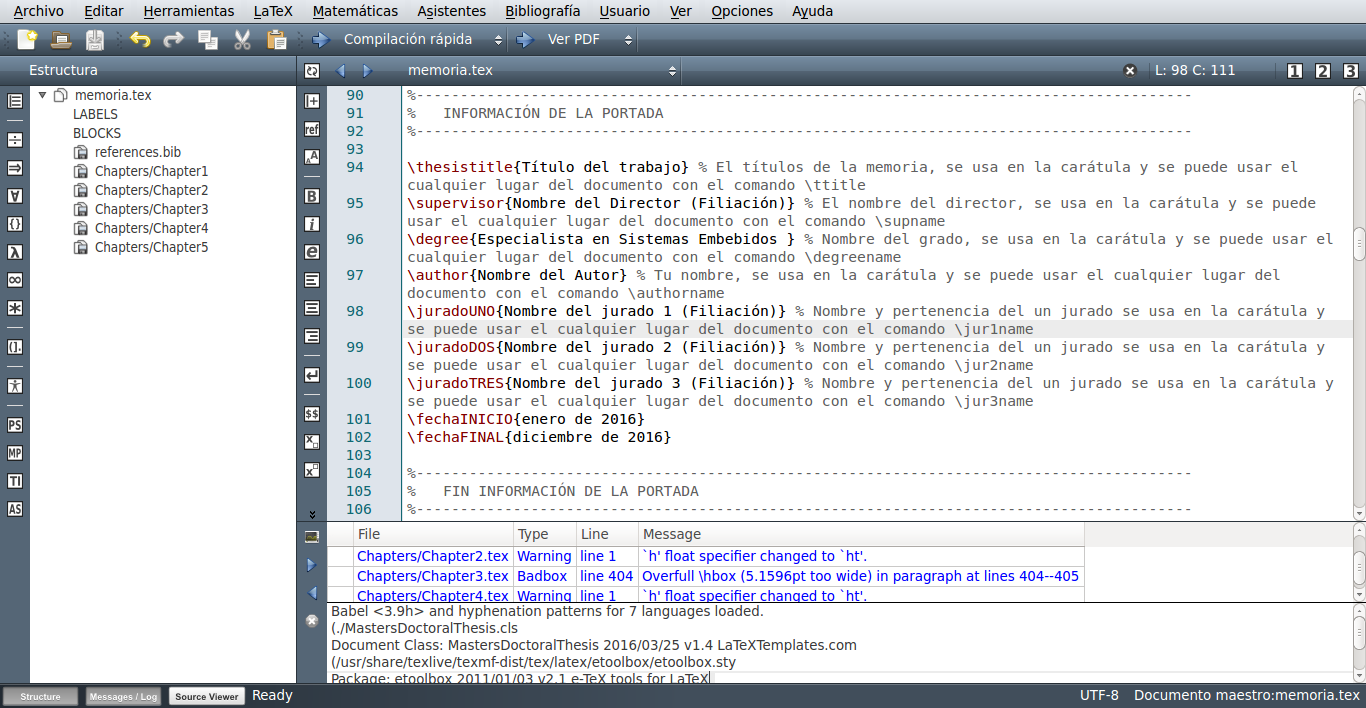
\includegraphics[width=\textwidth]{./Figures/texmaker.png}
	\caption{Entorno de trabajo del texMaker.}
	\label{fig:texmaker}
\end{figure}

Notar que existe una vista llamada Estructura a la izquierda de la interface que nos permite abrir desde dentro del programa los archivos individuales de los capítulos.  A la derecha se encuentra una vista con el archivo propiamente dicho para su edición. Hacia la parte inferior se encuentra una vista del log con información de los resultados de la compilación.  En esta última vista pueden aparecen advertencias o \textit{warning} que normalmente pueden ser ignorados y también los errores que se indican en color rojo.

Recordar que el archivo que se debe compilar con PDFLaTex es \file{memoria.tex}, si trataramos de compilar alguno de los capítulos directamente nos saldría un error.  Para salvar la molestia de tener que cambiar de archivo para compilar, se puede definer el archivo \file{memoria.tex} como ``documento maestro'' yendo al menú opciones -> ``definir documento actual como documento maestro'', lo que nos permite compilar cualquier archivo, sea memoria.tex, el capítulo donde estemos trabajando o incluso un apéndice si lo hubiera y texmaker se encargará automáticamente de compilar memoria.tex.

En el menú herramientas se encuentran las opciones de compilación.  Para producir un archivo PDF a partir de un archivo .tex se debe ejecutar PDFLaTeX (el shortcut es F6). Para incorporar nueva bibliografía se debe utilizar la opción BibTeX del mismo menú herramientas (el shortcut es F11).

Notar que para actualizar las tablas de contenidos se debe ejecutar PDFLaTeX dos veces.  Esto se debe a que es necesario actualizar algunos archivos auxiliares antes de obtener el resultado final.  En forma similar, para actualizar las referecias se debe ejecutar primero PDFLaTeX, después BibTeX y finalmente PDFLaTeX dos veces por idénticos motivos.

\section{Personalizando la plantilla en el archivo \file{memoria.tex}}
\label{sec:FillingFile}

Para personalizar la plantilla se debe incorporar la información propia en los distintos archivos \file{.tex}. 

Primero abrir \file{memoria.tex} con TexMaker (o el editor de su preferencia). Se debe ubicar dentro del archivo el bloque de código titulado \emph{INFORMACIÓN DE LA PORTADA} donde se deben incorporar los primeros datos personales con los que se constuirá automáticamente la portada.


%----------------------------------------------------------------------------------------

\section{El código del archivo \file{memoria.tex} explicado}

El archivo \file{memoria.tex} contiene la estructura de la memoria y se encuentra densamente comentado para explicar qué páginas, secciones y elementos de formato el código \LaTeX{} está creando en cada línea. Cada elemento de mayor jerarquía del documento está dividido en bloques con nombres en mayúsculas para que resulte evidente qué es lo que hace esa porción de código en particular. Inicialmente puede parecer que hay mucho código \LaTeX{}, pero es principalmente código para dar formato a la memoria y al estar ya definido, no requiere intervención del usuario de la plantilla.

Se debe comenzar por chequear que la información en la portada es correcta.

Luego viene el resumen que contiene una versión abreviada de su trabajo.  Se debería poder utilizar como un documento independiente para describir el contenido de su trabajo.

A continuación se encuentra la sección opcional de agradecimientos. 

El índice de contenidos, las listas de figura de tablas se generan en forma automática y no requieren intervención ni edición manual por parte del usuario de la plantilla. 

La siguiente página es opcional y puede contener una dedicatorio de una línea, en caso de que usted quiere dedicarle el trabajo a alguien.

Finalmente, se encuentra el bloque donde se incluyen los capítulos y los apéndices.  Por defecto se incluyen los 5 capítulos propuestos que se encuentran en la carpeta /Chapters. Cada capítulo se debe escribir en un archivo .tex separado y se debe poner en la carpeta \emph{Chapters} con el nombre \file{Chapter1}, \file{Chapter2}, etc\ldots El código para incluir capítulos desde archivos externos se muestra a continuación.

\begin{verbatim}
	% Chapter 1

\chapter{Introducción General} % Main chapter title

\label{Chapter1} % For referencing the chapter elsewhere, use \ref{Chapter1} 
\label{IntroGeneral}

%----------------------------------------------------------------------------------------

% Define some commands to keep the formatting separated from the content 
\newcommand{\keyword}[1]{\textbf{#1}}
\newcommand{\tabhead}[1]{\textbf{#1}}
\newcommand{\code}[1]{\texttt{#1}}
\newcommand{\file}[1]{\texttt{\bfseries#1}}
\newcommand{\option}[1]{\texttt{\itshape#1}}
\newcommand{\grados}{$^{\circ}$}

%----------------------------------------------------------------------------------------

%\section{Introducción}

%----------------------------------------------------------------------------------------
Aquí se exponen las problemáticas observadas que originaron el desarrollo del presente trabajo, junto con una breve descripción de la plataforma planteada para solucionarlas.
\section{Motivación}
Se observaron procesos de enseñanza, tanto en escuelas como en cursos de programación de sistemas embebidos. Se detectó que un gran obstáculo común entre alumnos es aprender en conjunto la lógica para resolución de problemas utilizando algoritmos, y la sintaxis de un lenguaje específico.
% Escuelas
\subsection{Robótica en la educación}
En el último tiempo se ha extendido cada vez más el uso de la robótica educativa como una herramienta particularmente útil en ámbitos escolares. Es utilizada como un sistema de enseñanza multidisciplinaria, que potencia el desarrollo de habilidades en las áreas de ciencias, tecnología, ingeniería y matemáticas. Correctamente estructurada, la robótica educativa permite incentivar el trabajo en equipo, el liderazgo, el emprendimiento y el aprendizaje a partir los errores.

La robótica en las escuelas se presenta entonces como una opción tecnológica e innovadora de afrontar la problemática de capturar el interés de los alumnos en los temas propuestos en la currícula. Esto se debe a la necesidad de involucrarse y trabajar en conjunto con sus pares para la resolución de problemas donde deben aplicar los conocimientos de las diferentes asignaturas. Al realizarse de manera entretenida los contenidos se fijan de manera más simple y natural.

Sin embargo, a la hora de aplicar estas técnicas de enseñanza se presenta una problemática. En el ambiente de las escuelas  primarias el público son estudiantes jóvenes en proceso de formación, que en general no poseen conocimientos técnicos en detalle como electrónica o manejo de lenguajes de programación. Esto se traduce en una limitación y dificultad a la hora de acercarse a este tipo de tecnologías, aunque el objetivo final no sea el aprendizaje de la robótica en sí misma sino utilizarla \textit{como herramienta}.

Las opciones actuales se presentan como plataformas que son, en su mayoría, diseños privativos, cerrados, con pocas posibilidades de modificación y en general desarrollos extranjeros importados a nuestro país. Se observa por lo tanto la necesidad de que la solución alternativa debe ser abierta y desarrollada localmente.

% Personas que se inician en los embebidos
\subsection{Introducción a la programación de sistemas embebidos}
Los primeros pasos para la inserción en el ámbito de la programación de sistemas embebidos pueden ser difíciles para algunas personas. Esto se debe, en parte, al hecho de tener que trabajar sobre plataformas diferentes a una PC y utilizando lenguajes de programación de bajo nivel (generalmente C o assembler).

Una de las mayores dificultades a la hora de iniciarse en la programación, de sistemas embebidos o en general, es la sintaxis específica del lenguaje que debe ser utilizado. Esto se evidencia a la hora de expresar en código la idea que se tiene, es decir la lógica del programa que se está desarrollando.

Una opción que presenta una curva de aprendizaje más plana es abstraerse, por lo menos en una primera etapa, del lenguaje que se utilizará para programar más adelante. De esta manera el alumno puede concentrarse en definir la lógica de su solución propuesta al problema planteado, sin preocuparse en cómo se expresaría en código (dicha tarea queda para etapas posteriores del proceso de aprendizaje).
%----------------------------------------------------------------------------------------

\section{Utilizando esta plantilla}

Si usted está familiarizado con \LaTeX{}, entonces puede explorar la estructura de directorios de esta plantilla y proceder a personalizarla agregando su información en el bloque \emph{INFORMACIÓN DE LA PORTADA} en el archivo \file{memoria.tex}.  

Se puede continuar luego modificando el resto de los archivos siguiendo los lineamientos que se describen en la sección \ref{sec:FillingFile} en la página \pageref{sec:FillingFile}.

Asegúrese de leer el capítulo \ref{Chapter2} acerca de las convenciones utilizadas para las Memoria de los Trabajos Finales de la Carrera de Especialización en Sistemas Embebidos de FIUBA.

Si es nuevo en \LaTeX{} se recomienda que continue leyendo el documento ya que contiene información básica para aprovechar el potencial de esta herramienta.


\subsection{Acerca de esta plantilla}

Esta plantilla \LaTeX{} está basada originalmente en torno a un archivo de estilo \LaTeX{} creado por Steve R.\ Gunn de la  University of Southampton (UK), department of Electronics and Computer Science. Se puede encontrar su trabajo original en el siguiente sitio de internet:
\url{http://www.ecs.soton.ac.uk/~srg/softwaretools/document/templates/}

El archivo de Gunn, \file{ecsthesis.cls} fue posteriormente modificado por Sunil Patel quien creó una plantilla esqueleto con la estructura de carpetas. El template resultante se puede encontrar en el sitio web de Sunil Patel:
\url{http://www.sunilpatel.co.uk/thesis-template}

El template de Patel se publicó a través de  \url{http://www.LaTeXTemplates.com} desde donde fue modificado muchas veces en base a solicitudes de usuarios. La versión 2.0 y subsiguientes representan cambios significativos respecto a la versión de la plantilla modificada por Patel, que es de hecho, dificilmente reconocible. El trabajo en la version 2.0 fue realizado por Vel Gayevskiy y Johannes Böttcher.

Uno de los primeros graduados de la Carerra de Especialización en Sistemas Embebios de la UBA, el Ing. \href{mailto:pbos@fi.uba.ar}{Patricio Bos} modificó los contenidos de la versión 2.3 para crear una plantilla altamente adaptada a la Carrera de Especialización de la UBA.

%----------------------------------------------------------------------------------------

\section{Qué incluye esta plantilla}

\subsection{Carpetas}

Esta plantilla se distribuye como una único archivo .zip que se puede descomprimir en varios archivos y carpetas. Los nombres de las carpetas son (o pretender ser) auto-explicativos.

\keyword{Appendices} -- Esta es la carpeta donde se deben poner los apéndices. Cada apéndice debe ir en su propio archivo \file{.tex}. Se incluye un ejemplo y una plantilla en la carpeta.

\keyword{Chapters} -- Esta es la carpeta donde se deben poner los capítulos de la memoria. Cada capítulo debe ir un su propio archivo \file{.tex} por separado.  Se ofrece por defecto, la siguiente estructura de capítulos y se recomienda su utilización dentro de lo posible:

\begin{itemize}
\item Capítulo 1: Introducción general	
\item Capítulo 2: Introducción específica
\item Capítulo 3: Diseño e implementación
\item Capítulo 4: Ensayos y resultados
\item Capítulo 5: Conclusiones

\end{itemize}

Esta estructura de capítulos es la que se recomienda para las memorias de la especialización.

\keyword{Figures} -- Esta carpeta contiene todas las figuras de la memoria.  Estas son las versiones finales de las imágenes que van a ser incluidas en la memoria.  Pueden ser imágenes en formato \textit{raster}\footnote{\url{https://en.wikipedia.org/wiki/Raster_graphics}} como \file{.png}, \file{.jpg} o en formato vectoriales\footnote{\url{https://en.wikipedia.org/wiki/Vector_graphics}} como \file{.pdf}, \file{.ps}.  Se debe notar que utilizar imágenes vectoriales disminuye notablemente el peso del documento final y acelera el tiempo de compilación por lo que es recomendable su utilización siempre que sea posible.

\subsection{Archivos}

También están incluidos varios archivos, la mayoría de ellos son de texto plano y se puede ver su contenido en un editor de texto. Después de la compilación inicial, se verá que más archivos auxiliares son creados por \ LaTeX{} o BibTeX, pero son de uso interno y que no es necesario eliminarlos o hacer nada con ellos.  Toda la información necesaria para complilar el documento se encuentra en los archivos \file{.tex} y en las imágenes de la carpeta Figures.

\keyword{referencias.bib} - este es un archivo importante que contiene toda la información bibliográfica y de referencias que se utilizará para las citas en la memoria en conjunto con BibTeX. Usted puede escribir las entradas bibliográficas en forma manual, aunque existen también programas de gestión de referencias que facilitan la creación y gestión de las referencias y permiten exportarlas en formato BibTeX.  También hay disponibles sitios web como \url{books.google.com} que permiten obtener toda la información necesaria para una cita en formato BibTeX.

\keyword{MastersDoctoralThesis.cls} -- este es un archivo importante. Es el archivos con la clase que le informa a \LaTeX{} cómo debe dar formato a la memoria. El usuario de la plantilla no debería necesitar modificar nada de este archivo.

\keyword{memoria.pdf} -- esta es su memoria con una tipografía bellamente compuesta (en formato de archivo PDF) creado por \LaTeX{}. Se distribuye con la plantilla y después de compilar por primera vez sin hacer ningún cambio se debería obtener una versión idéntica a este documento.

\keyword{memoria.tex} -- este es un archivo importante. Este es el archivo que tiene que compilar \LaTeX{} para producir la memoria como un archivo PDF. Contiene un marco de trabajo y estructuras que le indican a \LaTeX{} cómo diagramar la memoria.  Está altamente comentado para que se pueda entender qué es lo que realiza cada línea de código y por qué está incluida en ese lugar.  En este archivo se debe completar la información personalizada de las primeras sección según se indica en la sección \ref{sec:FillingFile}.

Archivos que \emph{no} forman parte de la distribución de la plantilla pero que son generados por \LaTeX{} como archivos auxiliares necesarios para la producción de la memoria.pdf son:

\keyword{memoria.aux} -- este es un archivo auxiliar generado por \LaTeX{}, si se borra \LaTeX{} simplemente lo regenera cuando se compila el archivo principal \file{memoria.tex}.

\keyword{memoria.bbl} -- este es un archivo auxiliar generado por BibTeX, si se borra BibTeX simplemente lo regenera cuando se compila el archivo principal \file{memoria.tex}. Mientras que el archivo \file{.bib} contiene todas las referencias que hay, este archivo \file{.bbl} contine sólo las referencias que han sido citadas y se utiliza para la construcción de la bibiografía.

\keyword{memoria.blg} -- este es un archivo auxiliar generado por BibTeX, si se borra BibTeX simplemente lo regenera cuando se compila el archivo principal \file{memoria.tex}.

\keyword{memoria.lof} -- este es un archivo auxiliar generado por \LaTeX{}, si se borra \LaTeX{} simplemente lo regenera cuando se compila el archivo principal \file{memoria.tex}.  Le indica a \LaTeX{} cómo construir la sección \emph{Lista de Figuras}.
 
\keyword{memoria.log} --  este es un archivo auxiliar generado por \LaTeX{}, si se borra \LaTeX{} simplemente lo regenera cuando se compila el archivo principal \file{memoria.tex}. Contiene mensajes de \LaTeX{}. Si se reciben errores o advertencias durante la compilación, se guardan en este archivo \file{.log}.

\keyword{memoria.lot} -- este es un archivo auxiliar generado por \LaTeX{}, si se borra \LaTeX{} simplemente lo regenera cuando se compila el archivo principal \file{memoria.tex}.  Le indica a \LaTeX{} cómo construir la sección \emph{Lista de Tablas}.

\keyword{memoria.out} -- este es un archivo auxiliar generado por \LaTeX{}, si se borra \LaTeX{} simplemente lo regenera cuando se compila el archivo principal \file{memoria.tex}.

De esta larga lista de archivos, sólo aquellos con la extensión \file{.bib}, \file{.cls} y \file{.tex} son importantes.  Los otros archivos auxiliares pueden ser ignorados o borrados ya que \LaTeX{} y BibTeX los regenerarán durante la compilación.

%----------------------------------------------------------------------------------------

\section{Entorno de trabajo}

Ante de comenzar a editar la plantilla debemos tener un editor \LaTeX{} instalado en nuestra computadora.  En forma análoga a lo que sucede en lenguaje C, que se puede crear y editar código con casi cualquier editor, exiten ciertos entornos de trabajo que nos pueden simplificar mucho la tarea.  En este sentido, se recomienda, sobre todo para los principiantes en \LaTeX{} la utilización de TexMaker, un programa gratuito y multi-plantaforma que está disponible tanto para windows como para sistemas GNU/linux.

La versión más reciente de TexMaker es la 4.5 y se puede descargar del siguiente link: \url{http://www.xm1math.net/texmaker/download.html}. Se puede consultar el manual de usuario en el siguiente link: \url{http://www.xm1math.net/texmaker/doc.html}.

\subsection{Configurando TexMaker}

La instalación de TexMaker se encarga de instalar todos los paquetes necesarios de \LaTeX{}. 
Una vez instalado el programa y abierto el archivo memoria.tex se debería ver una pantalla similar a la figura \ref{fig:texmaker}. 

\begin{figure}[h]
	\centering
	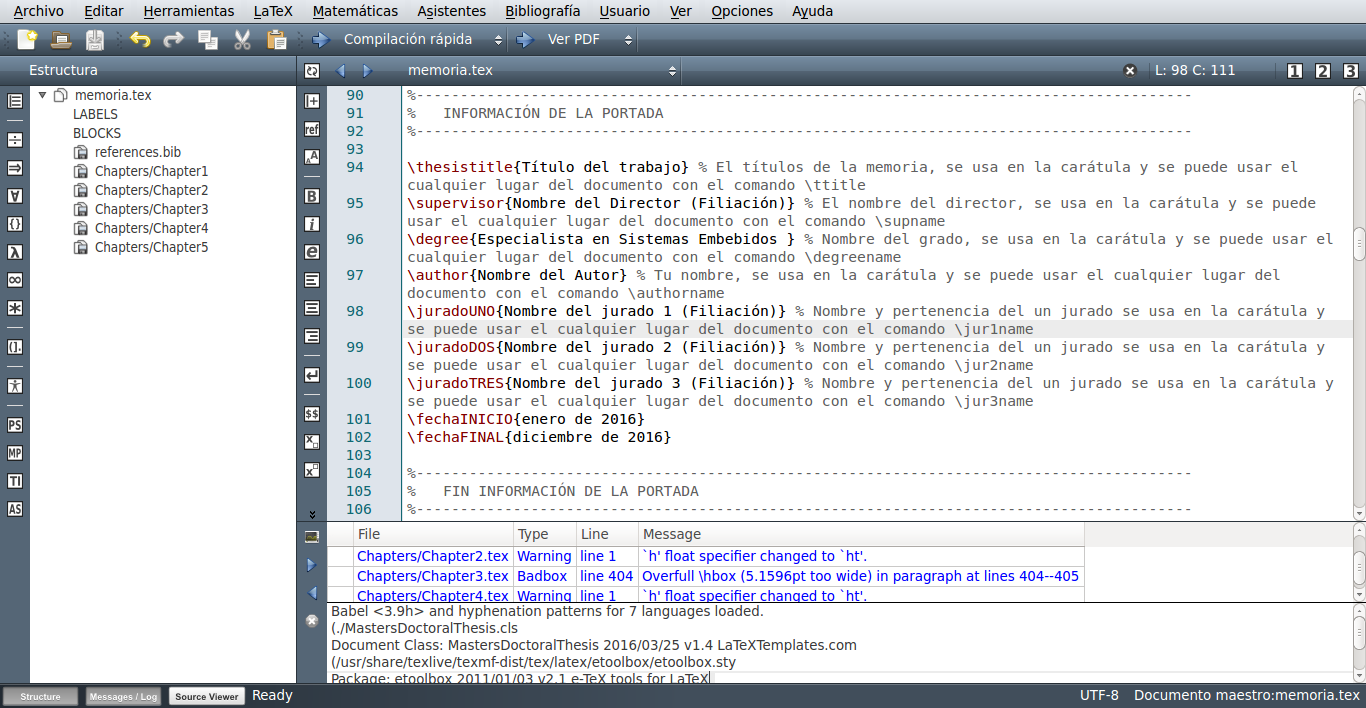
\includegraphics[width=\textwidth]{./Figures/texmaker.png}
	\caption{Entorno de trabajo del texMaker.}
	\label{fig:texmaker}
\end{figure}

Notar que existe una vista llamada Estructura a la izquierda de la interface que nos permite abrir desde dentro del programa los archivos individuales de los capítulos.  A la derecha se encuentra una vista con el archivo propiamente dicho para su edición. Hacia la parte inferior se encuentra una vista del log con información de los resultados de la compilación.  En esta última vista pueden aparecen advertencias o \textit{warning} que normalmente pueden ser ignorados y también los errores que se indican en color rojo.

Recordar que el archivo que se debe compilar con PDFLaTex es \file{memoria.tex}, si trataramos de compilar alguno de los capítulos directamente nos saldría un error.  Para salvar la molestia de tener que cambiar de archivo para compilar, se puede definer el archivo \file{memoria.tex} como ``documento maestro'' yendo al menú opciones -> ``definir documento actual como documento maestro'', lo que nos permite compilar cualquier archivo, sea memoria.tex, el capítulo donde estemos trabajando o incluso un apéndice si lo hubiera y texmaker se encargará automáticamente de compilar memoria.tex.

En el menú herramientas se encuentran las opciones de compilación.  Para producir un archivo PDF a partir de un archivo .tex se debe ejecutar PDFLaTeX (el shortcut es F6). Para incorporar nueva bibliografía se debe utilizar la opción BibTeX del mismo menú herramientas (el shortcut es F11).

Notar que para actualizar las tablas de contenidos se debe ejecutar PDFLaTeX dos veces.  Esto se debe a que es necesario actualizar algunos archivos auxiliares antes de obtener el resultado final.  En forma similar, para actualizar las referecias se debe ejecutar primero PDFLaTeX, después BibTeX y finalmente PDFLaTeX dos veces por idénticos motivos.

\section{Personalizando la plantilla en el archivo \file{memoria.tex}}
\label{sec:FillingFile}

Para personalizar la plantilla se debe incorporar la información propia en los distintos archivos \file{.tex}. 

Primero abrir \file{memoria.tex} con TexMaker (o el editor de su preferencia). Se debe ubicar dentro del archivo el bloque de código titulado \emph{INFORMACIÓN DE LA PORTADA} donde se deben incorporar los primeros datos personales con los que se constuirá automáticamente la portada.


%----------------------------------------------------------------------------------------

\section{El código del archivo \file{memoria.tex} explicado}

El archivo \file{memoria.tex} contiene la estructura de la memoria y se encuentra densamente comentado para explicar qué páginas, secciones y elementos de formato el código \LaTeX{} está creando en cada línea. Cada elemento de mayor jerarquía del documento está dividido en bloques con nombres en mayúsculas para que resulte evidente qué es lo que hace esa porción de código en particular. Inicialmente puede parecer que hay mucho código \LaTeX{}, pero es principalmente código para dar formato a la memoria y al estar ya definido, no requiere intervención del usuario de la plantilla.

Se debe comenzar por chequear que la información en la portada es correcta.

Luego viene el resumen que contiene una versión abreviada de su trabajo.  Se debería poder utilizar como un documento independiente para describir el contenido de su trabajo.

A continuación se encuentra la sección opcional de agradecimientos. 

El índice de contenidos, las listas de figura de tablas se generan en forma automática y no requieren intervención ni edición manual por parte del usuario de la plantilla. 

La siguiente página es opcional y puede contener una dedicatorio de una línea, en caso de que usted quiere dedicarle el trabajo a alguien.

Finalmente, se encuentra el bloque donde se incluyen los capítulos y los apéndices.  Por defecto se incluyen los 5 capítulos propuestos que se encuentran en la carpeta /Chapters. Cada capítulo se debe escribir en un archivo .tex separado y se debe poner en la carpeta \emph{Chapters} con el nombre \file{Chapter1}, \file{Chapter2}, etc\ldots El código para incluir capítulos desde archivos externos se muestra a continuación.

\begin{verbatim}
	% Chapter 1

\chapter{Introducción General} % Main chapter title

\label{Chapter1} % For referencing the chapter elsewhere, use \ref{Chapter1} 
\label{IntroGeneral}

%----------------------------------------------------------------------------------------

% Define some commands to keep the formatting separated from the content 
\newcommand{\keyword}[1]{\textbf{#1}}
\newcommand{\tabhead}[1]{\textbf{#1}}
\newcommand{\code}[1]{\texttt{#1}}
\newcommand{\file}[1]{\texttt{\bfseries#1}}
\newcommand{\option}[1]{\texttt{\itshape#1}}
\newcommand{\grados}{$^{\circ}$}

%----------------------------------------------------------------------------------------

%\section{Introducción}

%----------------------------------------------------------------------------------------
Aquí se exponen las problemáticas observadas que originaron el desarrollo del presente trabajo, junto con una breve descripción de la plataforma planteada para solucionarlas.
\section{Motivación}
Se observaron procesos de enseñanza, tanto en escuelas como en cursos de programación de sistemas embebidos. Se detectó que un gran obstáculo común entre alumnos es aprender en conjunto la lógica para resolución de problemas utilizando algoritmos, y la sintaxis de un lenguaje específico.
% Escuelas
\subsection{Robótica en la educación}
En el último tiempo se ha extendido cada vez más el uso de la robótica educativa como una herramienta particularmente útil en ámbitos escolares. Es utilizada como un sistema de enseñanza multidisciplinaria, que potencia el desarrollo de habilidades en las áreas de ciencias, tecnología, ingeniería y matemáticas. Correctamente estructurada, la robótica educativa permite incentivar el trabajo en equipo, el liderazgo, el emprendimiento y el aprendizaje a partir los errores.

La robótica en las escuelas se presenta entonces como una opción tecnológica e innovadora de afrontar la problemática de capturar el interés de los alumnos en los temas propuestos en la currícula. Esto se debe a la necesidad de involucrarse y trabajar en conjunto con sus pares para la resolución de problemas donde deben aplicar los conocimientos de las diferentes asignaturas. Al realizarse de manera entretenida los contenidos se fijan de manera más simple y natural.

Sin embargo, a la hora de aplicar estas técnicas de enseñanza se presenta una problemática. En el ambiente de las escuelas  primarias el público son estudiantes jóvenes en proceso de formación, que en general no poseen conocimientos técnicos en detalle como electrónica o manejo de lenguajes de programación. Esto se traduce en una limitación y dificultad a la hora de acercarse a este tipo de tecnologías, aunque el objetivo final no sea el aprendizaje de la robótica en sí misma sino utilizarla \textit{como herramienta}.

Las opciones actuales se presentan como plataformas que son, en su mayoría, diseños privativos, cerrados, con pocas posibilidades de modificación y en general desarrollos extranjeros importados a nuestro país. Se observa por lo tanto la necesidad de que la solución alternativa debe ser abierta y desarrollada localmente.

% Personas que se inician en los embebidos
\subsection{Introducción a la programación de sistemas embebidos}
Los primeros pasos para la inserción en el ámbito de la programación de sistemas embebidos pueden ser difíciles para algunas personas. Esto se debe, en parte, al hecho de tener que trabajar sobre plataformas diferentes a una PC y utilizando lenguajes de programación de bajo nivel (generalmente C o assembler).

Una de las mayores dificultades a la hora de iniciarse en la programación, de sistemas embebidos o en general, es la sintaxis específica del lenguaje que debe ser utilizado. Esto se evidencia a la hora de expresar en código la idea que se tiene, es decir la lógica del programa que se está desarrollando.

Una opción que presenta una curva de aprendizaje más plana es abstraerse, por lo menos en una primera etapa, del lenguaje que se utilizará para programar más adelante. De esta manera el alumno puede concentrarse en definir la lógica de su solución propuesta al problema planteado, sin preocuparse en cómo se expresaría en código (dicha tarea queda para etapas posteriores del proceso de aprendizaje).
%----------------------------------------------------------------------------------------

\section{Utilizando esta plantilla}

Si usted está familiarizado con \LaTeX{}, entonces puede explorar la estructura de directorios de esta plantilla y proceder a personalizarla agregando su información en el bloque \emph{INFORMACIÓN DE LA PORTADA} en el archivo \file{memoria.tex}.  

Se puede continuar luego modificando el resto de los archivos siguiendo los lineamientos que se describen en la sección \ref{sec:FillingFile} en la página \pageref{sec:FillingFile}.

Asegúrese de leer el capítulo \ref{Chapter2} acerca de las convenciones utilizadas para las Memoria de los Trabajos Finales de la Carrera de Especialización en Sistemas Embebidos de FIUBA.

Si es nuevo en \LaTeX{} se recomienda que continue leyendo el documento ya que contiene información básica para aprovechar el potencial de esta herramienta.


\subsection{Acerca de esta plantilla}

Esta plantilla \LaTeX{} está basada originalmente en torno a un archivo de estilo \LaTeX{} creado por Steve R.\ Gunn de la  University of Southampton (UK), department of Electronics and Computer Science. Se puede encontrar su trabajo original en el siguiente sitio de internet:
\url{http://www.ecs.soton.ac.uk/~srg/softwaretools/document/templates/}

El archivo de Gunn, \file{ecsthesis.cls} fue posteriormente modificado por Sunil Patel quien creó una plantilla esqueleto con la estructura de carpetas. El template resultante se puede encontrar en el sitio web de Sunil Patel:
\url{http://www.sunilpatel.co.uk/thesis-template}

El template de Patel se publicó a través de  \url{http://www.LaTeXTemplates.com} desde donde fue modificado muchas veces en base a solicitudes de usuarios. La versión 2.0 y subsiguientes representan cambios significativos respecto a la versión de la plantilla modificada por Patel, que es de hecho, dificilmente reconocible. El trabajo en la version 2.0 fue realizado por Vel Gayevskiy y Johannes Böttcher.

Uno de los primeros graduados de la Carerra de Especialización en Sistemas Embebios de la UBA, el Ing. \href{mailto:pbos@fi.uba.ar}{Patricio Bos} modificó los contenidos de la versión 2.3 para crear una plantilla altamente adaptada a la Carrera de Especialización de la UBA.

%----------------------------------------------------------------------------------------

\section{Qué incluye esta plantilla}

\subsection{Carpetas}

Esta plantilla se distribuye como una único archivo .zip que se puede descomprimir en varios archivos y carpetas. Los nombres de las carpetas son (o pretender ser) auto-explicativos.

\keyword{Appendices} -- Esta es la carpeta donde se deben poner los apéndices. Cada apéndice debe ir en su propio archivo \file{.tex}. Se incluye un ejemplo y una plantilla en la carpeta.

\keyword{Chapters} -- Esta es la carpeta donde se deben poner los capítulos de la memoria. Cada capítulo debe ir un su propio archivo \file{.tex} por separado.  Se ofrece por defecto, la siguiente estructura de capítulos y se recomienda su utilización dentro de lo posible:

\begin{itemize}
\item Capítulo 1: Introducción general	
\item Capítulo 2: Introducción específica
\item Capítulo 3: Diseño e implementación
\item Capítulo 4: Ensayos y resultados
\item Capítulo 5: Conclusiones

\end{itemize}

Esta estructura de capítulos es la que se recomienda para las memorias de la especialización.

\keyword{Figures} -- Esta carpeta contiene todas las figuras de la memoria.  Estas son las versiones finales de las imágenes que van a ser incluidas en la memoria.  Pueden ser imágenes en formato \textit{raster}\footnote{\url{https://en.wikipedia.org/wiki/Raster_graphics}} como \file{.png}, \file{.jpg} o en formato vectoriales\footnote{\url{https://en.wikipedia.org/wiki/Vector_graphics}} como \file{.pdf}, \file{.ps}.  Se debe notar que utilizar imágenes vectoriales disminuye notablemente el peso del documento final y acelera el tiempo de compilación por lo que es recomendable su utilización siempre que sea posible.

\subsection{Archivos}

También están incluidos varios archivos, la mayoría de ellos son de texto plano y se puede ver su contenido en un editor de texto. Después de la compilación inicial, se verá que más archivos auxiliares son creados por \ LaTeX{} o BibTeX, pero son de uso interno y que no es necesario eliminarlos o hacer nada con ellos.  Toda la información necesaria para complilar el documento se encuentra en los archivos \file{.tex} y en las imágenes de la carpeta Figures.

\keyword{referencias.bib} - este es un archivo importante que contiene toda la información bibliográfica y de referencias que se utilizará para las citas en la memoria en conjunto con BibTeX. Usted puede escribir las entradas bibliográficas en forma manual, aunque existen también programas de gestión de referencias que facilitan la creación y gestión de las referencias y permiten exportarlas en formato BibTeX.  También hay disponibles sitios web como \url{books.google.com} que permiten obtener toda la información necesaria para una cita en formato BibTeX.

\keyword{MastersDoctoralThesis.cls} -- este es un archivo importante. Es el archivos con la clase que le informa a \LaTeX{} cómo debe dar formato a la memoria. El usuario de la plantilla no debería necesitar modificar nada de este archivo.

\keyword{memoria.pdf} -- esta es su memoria con una tipografía bellamente compuesta (en formato de archivo PDF) creado por \LaTeX{}. Se distribuye con la plantilla y después de compilar por primera vez sin hacer ningún cambio se debería obtener una versión idéntica a este documento.

\keyword{memoria.tex} -- este es un archivo importante. Este es el archivo que tiene que compilar \LaTeX{} para producir la memoria como un archivo PDF. Contiene un marco de trabajo y estructuras que le indican a \LaTeX{} cómo diagramar la memoria.  Está altamente comentado para que se pueda entender qué es lo que realiza cada línea de código y por qué está incluida en ese lugar.  En este archivo se debe completar la información personalizada de las primeras sección según se indica en la sección \ref{sec:FillingFile}.

Archivos que \emph{no} forman parte de la distribución de la plantilla pero que son generados por \LaTeX{} como archivos auxiliares necesarios para la producción de la memoria.pdf son:

\keyword{memoria.aux} -- este es un archivo auxiliar generado por \LaTeX{}, si se borra \LaTeX{} simplemente lo regenera cuando se compila el archivo principal \file{memoria.tex}.

\keyword{memoria.bbl} -- este es un archivo auxiliar generado por BibTeX, si se borra BibTeX simplemente lo regenera cuando se compila el archivo principal \file{memoria.tex}. Mientras que el archivo \file{.bib} contiene todas las referencias que hay, este archivo \file{.bbl} contine sólo las referencias que han sido citadas y se utiliza para la construcción de la bibiografía.

\keyword{memoria.blg} -- este es un archivo auxiliar generado por BibTeX, si se borra BibTeX simplemente lo regenera cuando se compila el archivo principal \file{memoria.tex}.

\keyword{memoria.lof} -- este es un archivo auxiliar generado por \LaTeX{}, si se borra \LaTeX{} simplemente lo regenera cuando se compila el archivo principal \file{memoria.tex}.  Le indica a \LaTeX{} cómo construir la sección \emph{Lista de Figuras}.
 
\keyword{memoria.log} --  este es un archivo auxiliar generado por \LaTeX{}, si se borra \LaTeX{} simplemente lo regenera cuando se compila el archivo principal \file{memoria.tex}. Contiene mensajes de \LaTeX{}. Si se reciben errores o advertencias durante la compilación, se guardan en este archivo \file{.log}.

\keyword{memoria.lot} -- este es un archivo auxiliar generado por \LaTeX{}, si se borra \LaTeX{} simplemente lo regenera cuando se compila el archivo principal \file{memoria.tex}.  Le indica a \LaTeX{} cómo construir la sección \emph{Lista de Tablas}.

\keyword{memoria.out} -- este es un archivo auxiliar generado por \LaTeX{}, si se borra \LaTeX{} simplemente lo regenera cuando se compila el archivo principal \file{memoria.tex}.

De esta larga lista de archivos, sólo aquellos con la extensión \file{.bib}, \file{.cls} y \file{.tex} son importantes.  Los otros archivos auxiliares pueden ser ignorados o borrados ya que \LaTeX{} y BibTeX los regenerarán durante la compilación.

%----------------------------------------------------------------------------------------

\section{Entorno de trabajo}

Ante de comenzar a editar la plantilla debemos tener un editor \LaTeX{} instalado en nuestra computadora.  En forma análoga a lo que sucede en lenguaje C, que se puede crear y editar código con casi cualquier editor, exiten ciertos entornos de trabajo que nos pueden simplificar mucho la tarea.  En este sentido, se recomienda, sobre todo para los principiantes en \LaTeX{} la utilización de TexMaker, un programa gratuito y multi-plantaforma que está disponible tanto para windows como para sistemas GNU/linux.

La versión más reciente de TexMaker es la 4.5 y se puede descargar del siguiente link: \url{http://www.xm1math.net/texmaker/download.html}. Se puede consultar el manual de usuario en el siguiente link: \url{http://www.xm1math.net/texmaker/doc.html}.

\subsection{Configurando TexMaker}

La instalación de TexMaker se encarga de instalar todos los paquetes necesarios de \LaTeX{}. 
Una vez instalado el programa y abierto el archivo memoria.tex se debería ver una pantalla similar a la figura \ref{fig:texmaker}. 

\begin{figure}[h]
	\centering
	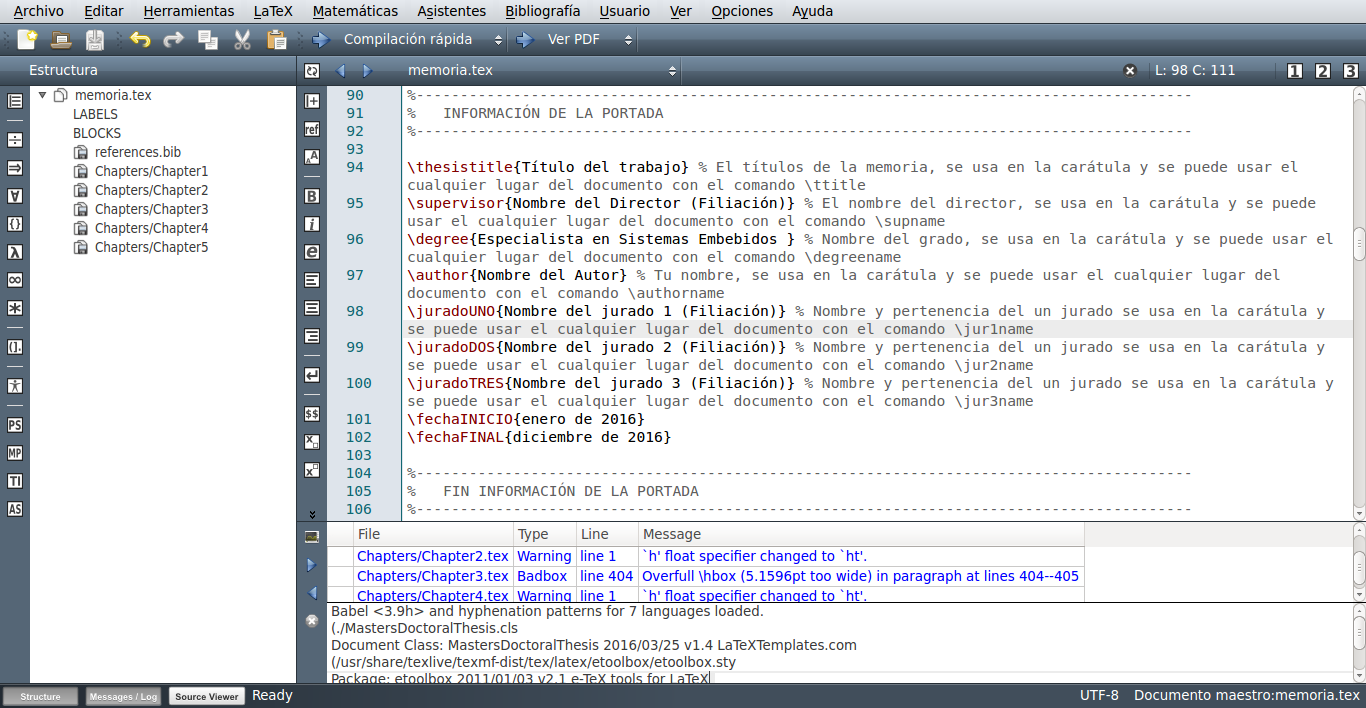
\includegraphics[width=\textwidth]{./Figures/texmaker.png}
	\caption{Entorno de trabajo del texMaker.}
	\label{fig:texmaker}
\end{figure}

Notar que existe una vista llamada Estructura a la izquierda de la interface que nos permite abrir desde dentro del programa los archivos individuales de los capítulos.  A la derecha se encuentra una vista con el archivo propiamente dicho para su edición. Hacia la parte inferior se encuentra una vista del log con información de los resultados de la compilación.  En esta última vista pueden aparecen advertencias o \textit{warning} que normalmente pueden ser ignorados y también los errores que se indican en color rojo.

Recordar que el archivo que se debe compilar con PDFLaTex es \file{memoria.tex}, si trataramos de compilar alguno de los capítulos directamente nos saldría un error.  Para salvar la molestia de tener que cambiar de archivo para compilar, se puede definer el archivo \file{memoria.tex} como ``documento maestro'' yendo al menú opciones -> ``definir documento actual como documento maestro'', lo que nos permite compilar cualquier archivo, sea memoria.tex, el capítulo donde estemos trabajando o incluso un apéndice si lo hubiera y texmaker se encargará automáticamente de compilar memoria.tex.

En el menú herramientas se encuentran las opciones de compilación.  Para producir un archivo PDF a partir de un archivo .tex se debe ejecutar PDFLaTeX (el shortcut es F6). Para incorporar nueva bibliografía se debe utilizar la opción BibTeX del mismo menú herramientas (el shortcut es F11).

Notar que para actualizar las tablas de contenidos se debe ejecutar PDFLaTeX dos veces.  Esto se debe a que es necesario actualizar algunos archivos auxiliares antes de obtener el resultado final.  En forma similar, para actualizar las referecias se debe ejecutar primero PDFLaTeX, después BibTeX y finalmente PDFLaTeX dos veces por idénticos motivos.

\section{Personalizando la plantilla en el archivo \file{memoria.tex}}
\label{sec:FillingFile}

Para personalizar la plantilla se debe incorporar la información propia en los distintos archivos \file{.tex}. 

Primero abrir \file{memoria.tex} con TexMaker (o el editor de su preferencia). Se debe ubicar dentro del archivo el bloque de código titulado \emph{INFORMACIÓN DE LA PORTADA} donde se deben incorporar los primeros datos personales con los que se constuirá automáticamente la portada.


%----------------------------------------------------------------------------------------

\section{El código del archivo \file{memoria.tex} explicado}

El archivo \file{memoria.tex} contiene la estructura de la memoria y se encuentra densamente comentado para explicar qué páginas, secciones y elementos de formato el código \LaTeX{} está creando en cada línea. Cada elemento de mayor jerarquía del documento está dividido en bloques con nombres en mayúsculas para que resulte evidente qué es lo que hace esa porción de código en particular. Inicialmente puede parecer que hay mucho código \LaTeX{}, pero es principalmente código para dar formato a la memoria y al estar ya definido, no requiere intervención del usuario de la plantilla.

Se debe comenzar por chequear que la información en la portada es correcta.

Luego viene el resumen que contiene una versión abreviada de su trabajo.  Se debería poder utilizar como un documento independiente para describir el contenido de su trabajo.

A continuación se encuentra la sección opcional de agradecimientos. 

El índice de contenidos, las listas de figura de tablas se generan en forma automática y no requieren intervención ni edición manual por parte del usuario de la plantilla. 

La siguiente página es opcional y puede contener una dedicatorio de una línea, en caso de que usted quiere dedicarle el trabajo a alguien.

Finalmente, se encuentra el bloque donde se incluyen los capítulos y los apéndices.  Por defecto se incluyen los 5 capítulos propuestos que se encuentran en la carpeta /Chapters. Cada capítulo se debe escribir en un archivo .tex separado y se debe poner en la carpeta \emph{Chapters} con el nombre \file{Chapter1}, \file{Chapter2}, etc\ldots El código para incluir capítulos desde archivos externos se muestra a continuación.

\begin{verbatim}
	\include{Chapters/Chapter1}
	\include{Chapters/Chapter2} 
	\include{Chapters/Chapter3}
	\include{Chapters/Chapter4} 
	\include{Chapters/Chapter5} 
\end{verbatim}

Los apéndices también deben ir en archivos .tex separados y se deben ubicar dentro de la carpeta \emph{Appendices}. Los apéndices vienen comentados con el caracter \code{\%} por defecto y para incluirlos se debe eliminar dicho caracter.

Luego del preambulo, los capítulos y los apéndices, finalmente viene la bibliografía. El estilo bibliográfico (llamado \option{authoryear}) es utilizado por \LaTeX{} para generar las referencias y es un estilo con todas las características necesarias para su composición.  No se debe subestimar lo agradecido que estarán sus lectores al encontrar que las referencias se encuentran a un clic de distancia.  Por supuesto, esto depende de que usted haya puesto la url correspondiente en el archivo BibTex en primer lugar.

%----------------------------------------------------------------------------------------







	\chapter{Introducción Específica} % Main chapter title

\label{Chapter2}
En este capítulo se presenta CIAABOT con más detalle, incluyendo especificaciones técnicas sobre la plataforma utilizada. Se establecen los requerimientos planteados y la planificación para el desarrollo del trabajo.

\section{CIAABOT: Partes componentes}
\label{sec:ciaabot:partes}
Se planteó que para lograr los objetivos propuestos, la plataforma debería estar formada por tres partes fundamentales, que funcionarían complementadas para armar un ecosistema CIAABOT, como está esquematizado en la figura \ref{fig:ciaabot:partes}. A continuación se describirá cada uno de ellos.

\begin{center}
    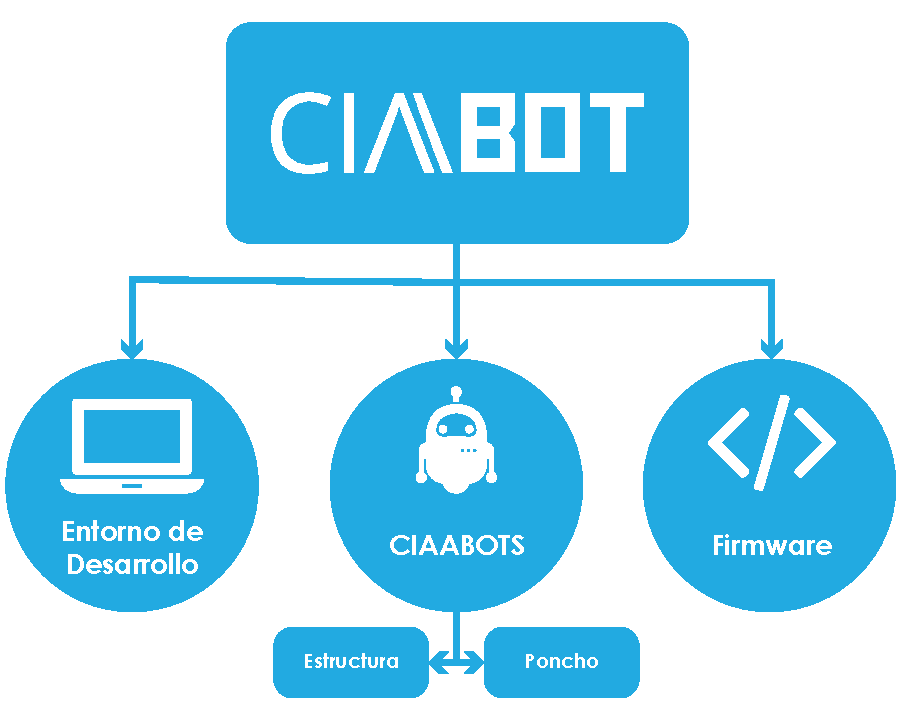
\includegraphics[scale=.8]{./Figures/ciaabot-partes.pdf}
    \label{fig:ciaabot:partes}
    \captionof{figure}{Diagrama de las partes que componen CIAABOT.}
\end{center}


\subsection{Entorno de desarrollo integrado}
\label{subsec:ide}
Un IDE (\emph{Integrated Development Environment}, Entorno de Desarrollo Integrado) es un software que incluye varias herramientas para asistir a los desarrolladores con su trabajo. Generalmente incluye algún editor para el código, herramientas de construcción o compilación automáticas, programación de la plataforma y posible depuración.

El CIAABOT-IDE es el centro del trabajo de los usuarios. Aquí plasman sus ideas y soluciones a problemas planteados. Esto lo hacen por medio de un editor de código en el que utilizan bloques predefinidos y no texto, como se observa en la figura \ref{fig:ciaabot:ide}. Arrastrando e interconectando los mismos logran definir la lógica para su programa.

Una opción interesante para remarcar es la salida de código en C. Cada vez que se modifica el diagrama de bloques, el código en C producido se modifica en tiempo real. Esto es muy útil para gente que pretende aprender a programar en C, ya que ve de manera directa cómo afecta cada bloque a las líneas de código y puede apreciar las equivalencias.

La plataforma también permite compilar y luego descargar el código generado en la placa solamente conectándola por USB.

Una vez que se finalizó el trabajo se puede guardar el proyecto en un archivo \emph{.cbp} que contiene la estructura de bloques en la que se estuvo trabajando, junto con las opciones adicionales del proyecto. Este archivo puede ser compartido y abierto en otra PC para ser reutilizado o modificado y guardado nuevamente.

Otra de las opciones que fue publicada en la última versión de CIAABOT-IDE (v0.0.8) es la de seleccionar los directorios de búsqueda para el toolchain. Las aplicaciones necesarias para todos los sistemas operativos son dos: El compilador arm-none-eabi-gcc y el debugger openOCD. Adicionalmente, en Windows se requieren otros ejecutables como make, para poder compilar y descargar el programa.

\begin{figure}[h]
	\centering
	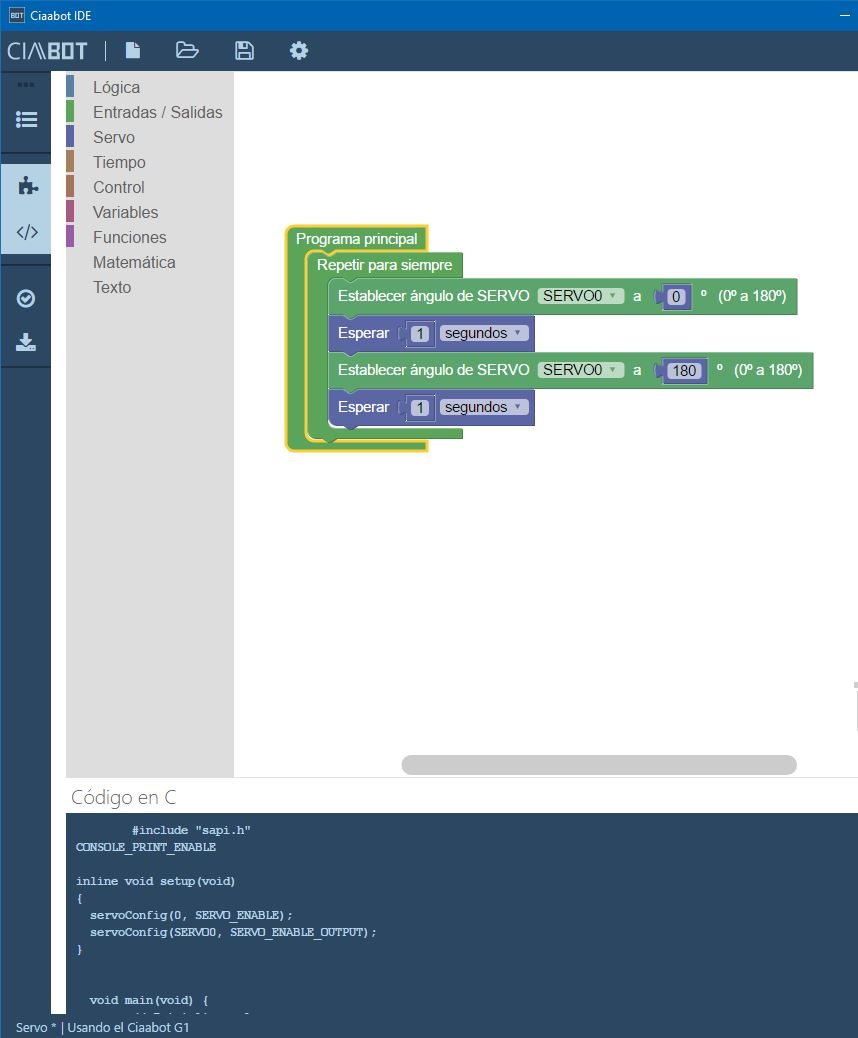
\includegraphics[scale=.5]{./Figures/ciaabot-ide-bloques.jpg}
	\caption{Editor gráfico de CIAABOT-IDE.}
	\label{fig:ciaabot:ide}
\end{figure}

\subsection{CIAABOTS}
\label{subsec:ciaabots}
Los robots que funcionen bajo esta plataforma serán denominados \emph{CIAABOTS}. Siguiendo la idea original de que CIAABOT sea utilizada en escuelas o por entusiastas, se planteó que estos robots estén diseñados estructuralmente para poder ser impresos con impresoras 3D.

De esta manera es posible enviar los archivos para imprimirlos en cualquier escuela que cuente con este sistema de impresión para replicarlo. Sólo sería necesario tener la placa CIAA correspondiente al modelo, armar el poncho (de diseño abierto) y adquirir en algún lugar de conveniencia los actuadores o sensores particulares del CIAABOT (motores DC, sensores IR, ultrasonido, etc.).

El diseño del poncho para el primer modelo de CIAABOT, el G1 se puede encontrar en github \citep{CIAABOT:G1}, realizado con el suite KiCad como todos los diseños relacionados al proyecto CIAA.

\subsection{Firmware}
\label{subsec:firmware}
CIAABOT utiliza como base para su firmware dos proyectos principales del ecosistema CIAA: Firmware v2 \citep{CIAA:firmwarev2} y sAPI \citep{sAPI}. En conjunto proveen una forma simplificada de programar las placas CIAA.

La sAPI es una HAL (\emph{Hardware Abstraction Layer}, Capa de Abstracción de Hardware) para los microcontroladores, que permite acceder de manera simple a varios de los diferentes periféricos.

Juntando varias funciones de la sAPI es posible armar funciones más complejas de mayor nivel para manejar características más específicas de cada modelo de CIAABOT.

Se prevé que con el avance del desarrollo de la plataforma cada modelo tendrá bloques específicos que estarán disponibles en el editor, cuando se lo seleccione a la hora de armar el proyecto en el IDE. Así, podrían armarse bloques que realicen por ejemplo una lectura de un sensor, que implicaría el manejo de pines y tiempos de espera.

\section{Plataforma utilizada}
\label{sec:plataforma}
Como base para el proyecto se optó por utilizar CIAA. Es un proyecto centrado en el trabajo colaborativo que busca la innovación para crear, diseñar y desarrollar soluciones electrónicas en la industria. Dentro de sus objetivos se encuentran:

\begin{itemize}
\item Impulsar el desarrollo tecnológico nacional, a partir de sumar valor agregado al trabajo y a los productos y servicios, mediante el uso de sistemas electrónicos, en el marco de la vinculación de las instituciones educativas y el sistema científico-tecnológico con la industria.

\item Darle visibilidad positiva a la electrónica argentina.

\item Generar cambios estructurales en la forma en la que se desarrollan y utilizan en nuestro país los conocimientos en el ámbito de la electrónica y de las instituciones y empresas que hacen uso de ella. \citep{CIAA:wiki}
\end{itemize}

Se utiliza esta plataforma por compartir la misma idea de ser un proyecto libre, poseer una creciente comunidad e incentivar la industria nacional. Se consideró que es un proyecto suficientemente maduro y con actualizaciones y desarrollos constantes como para ser utilizado de base.

\subsection{EDU-CIAA-NXP}
\label{subsec:eduCiaaNxp}
La EDU-CIAA-NXP es la versión educativa y de bajo costo de la CIAA-NXP. Utiliza, al igual que la CIAA-NXP, el microcontrolador LPC4337 de NXP, un doble núcleo ARM Cortex-M4F y Cortex M0. Como se observa en la figura \ref{fig:eduCiaaNxp}, la placa posee 4 leds y 4 pulsadores de hardware adicional. Para ampliar sus capacidades se utilizan los conectores laterales, para adicionar alguna placa extensora llamada \emph{Poncho}.

\begin{figure}[h]
\centering
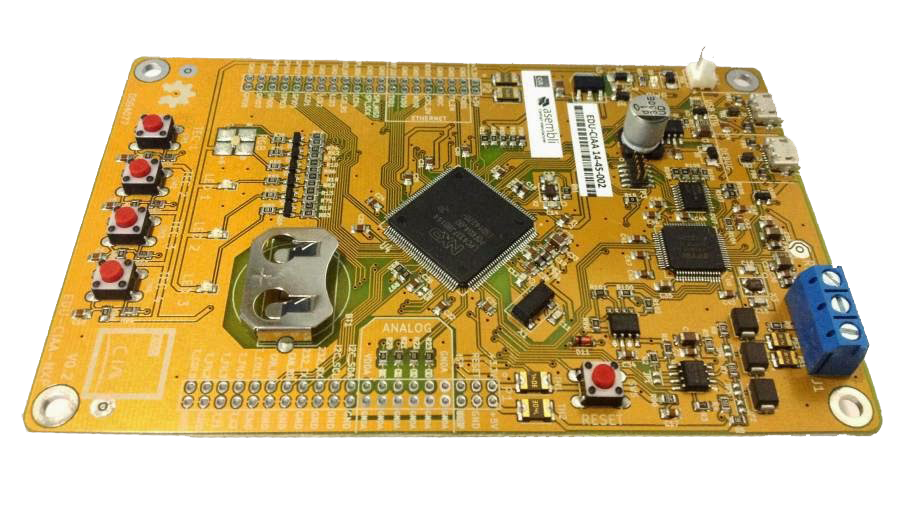
\includegraphics[scale=.5]{./Figures/edu-ciaa-nxp.png}
\caption{Placa EDU-CIAA-NXP}
\label{fig:eduCiaaNxp}
\end{figure}

Permite realizar programación y debugging, así como también acceder a una de sus UARTs, por medio de USB. Además posee otro puerto para que la placa funcione en modo OTG (\emph{On The Go}).

\section{Requerimientos}
\label{sec:requerimientos}
Se plantearon requerimientos que el proyecto debería cumplir a la hora de ser entregado. Se evaluaron sus posibilidades y se clasificaron en categorías.

\subsection{Requerimientos del sistema}
\label{subsec:requerimientosSistema}
Se estableció que el IDE debería poder ejecutarse como mínimo en un entorno Linux o Windows. Por la orientación didáctica del proyecto su uso debería ser simple, amigable y didáctico. Además, la programación debería poder realizarse íntegramente de manera gráfica por medio de bloques, donde cada uno represente acciones simples.

El IDE debería permitir un manejo de proyectos en forma de archivos, que posibilitaran el guardado y distribución de los mismos. Dentro de las opciones del proyecto debería poder seleccionarse el modelo de CIAABOT utilizado. Actualmente la opción existe, pero hay un solo modelo disponible.

El algoritmo que se genera a partir de los bloques debería estar disponible en lenguaje C, poder compilarse y programarse desde la aplicación, por puerto USB.

\subsection{Componentes del Sistema}
\label{subsec:componentesSistema}
Como ya se mencionó, se debería utilizar en principio la placa EDU-CIAA-NXP, y un poncho si fuese necesario para controlar la maqueta o robot implementado para la muestra. En el diseño de este poncho todos los periféricos deberían funcionar independientes al resto.

\subsection{Firmware}
\label{subsec:firmware}
Para el desarrollo del software se implementaría un sistema de control de versiones. Para la programación de los robots se utilizarían dos bibliotecas: En C la mencionada sAPI, y una de Firmata para un monitoreo del mismo por medio del puerto serie, con un cliente corriendo en la placa.

\subsection{Procesos Finales}
\label{subsec:procesosFinales}
Se requiere un manual de uso e instalación, junto con ejemplos básicos y funcionales, que sean representativos de las características de la plataforma. Se implementaría sobre una maqueta o robot adaptado a la EDU-CIAA, y con ello se evaluarían los resultados del proyecto y su aplicación en ámbitos de enseñanza reales.

\section{Planificación}
\label{sec:planificacion}
\subsection{Desglose en tareas}
En primer lugar, para definir objetivos concretos, se planteó una serie de entregables para el proyecto:

\begin{itemize}
\item IDE en funcionamiento.
\item Poncho CIAABOT G1 diseñado enteramente.
\item Manual de uso, instalación y ejemplos funcionales.
\item El presente informe final.
\end{itemize}

Siguiendo los lineamientos de las estrategias vistas en la materia Gestión de Proyectos, se procedió al diseño de una lista de desglose del trabajo en tareas. Se estimó un tiempo aproximado de 615 horas, distribuidas en grupos de tareas de la siguiente manera:

\begin{itemize}
\item Planificación del proyecto (40 hs.).
\item Investigación preliminar (45 hs.).
\item Selección de bibliotecas y plataformas (30 hs.).
\item Desarrollo de la aplicación de escritorio (45 hs.).
\item Desarrollo del editor gráfico (55 hs.).
\item Programación por USB y monitoreo (60 hs.).
\item Desarrollo del hardware (100 hs.).
\item Desarrollo del firmware (70 hs.).
\item Integración del sistema (50 hs.).
\item Procesos finales (120 hs.).
\end{itemize}
 
	\chapter{Diseño e Implementación} % Main chapter title

\label{Chapter3} % Change X to a consecutive number; for referencing this chapter elsewhere, use \ref{ChapterX}
\definecolor{mygreen}{rgb}{0,0.6,0}
\definecolor{mygray}{rgb}{0.5,0.5,0.5}
\definecolor{mymauve}{rgb}{0.58,0,0.82}

\lstset{ %
  backgroundcolor=\color{white},   % choose the background color; you must add \usepackage{color} or \usepackage{xcolor}
  basicstyle=\footnotesize,        % the size of the fonts that are used for the code
  breakatwhitespace=false,         % sets if automatic breaks should only happen at whitespace
  breaklines=true,                 % sets automatic line breaking
  captionpos=b,                    % sets the caption-position to bottom
  commentstyle=\color{mygreen},    % comment style
  deletekeywords={...},            % if you want to delete keywords from the given language
  %escapeinside={\%*}{*)},          % if you want to add LaTeX within your code
  %extendedchars=true,              % lets you use non-ASCII characters; for 8-bits encodings only, does not work with UTF-8
  %frame=single,	                   % adds a frame around the code
  keepspaces=true,                 % keeps spaces in text, useful for keeping indentation of code (possibly needs columns=flexible)
  keywordstyle=\color{blue},       % keyword style
  language=[ANSI]C,					% the language of the code
  %otherkeywords={*,...},           % if you want to add more keywords to the set
  numbers=left,                    % where to put the line-numbers; possible values are (none, left, right)
  numbersep=5pt,                   % how far the line-numbers are from the code
  numberstyle=\tiny\color{mygray}, % the style that is used for the line-numbers
  rulecolor=\color{black},         % if not set, the frame-color may be changed on line-breaks within not-black text (e.g. comments (green here))
  showspaces=false,                % show spaces everywhere adding particular underscores; it overrides 'showstringspaces'
  showstringspaces=false,          % underline spaces within strings only
  showtabs=false,                  % show tabs within strings adding particular underscores
  stepnumber=1,                    % the step between two line-numbers. If it's 1, each line will be numbered
  stringstyle=\color{mymauve},     % string literal style
  tabsize=2,	                   % sets default tabsize to 2 spaces
  title=\lstname,                   % show the filename of files included with \lstinputlisting; also try caption instead of title
  morecomment=[s]{/*}{*/}%
}


%----------------------------------------------------------------------------------------
%	SECTION 1
%----------------------------------------------------------------------------------------
\section{Estructura del Software}

sAPI
\begin{itemize}
\item Interrupciones.
\item SysTick.
\item GPIO.
\item UART.
\item ADC.
\item DAC.
\item $I^2C$.
\item SPI.
\item RTC.
\item SCT.
\item Timers.
\end{itemize}

Además incluye funciones avanzadas de conversión de datos, impresión formateada por UART, manejo de displays 7 segmentos, teclados matriciales, servos y PWM entre otras.

%----------------------------------------------------------------------------------------
La idea de esta sección es resaltar los problemas encontrados, los criterios utilizados y la justificación de las decisiones que se hayan tomado.

Se puede agregar código o pseudocódigo dentro de un entorno lstlisting con el siguiente código:

\begin{verbatim}
\begin{lstlisting}[caption= "un epígrafe descriptivo"]

	las líneas de código irían aquí...
	
\end{lstlisting}
\end{verbatim}

A modo de ejemplo:

\begin{lstlisting}[caption=Pseudocódigo del lazo principal de control.]  % Start your code-block

#define MAX_SENSOR_NUMBER 3
#define MAX_ALARM_NUMBER  6
#define MAX_ACTUATOR_NUMBER 6

uint32_t sensorValue[MAX_SENSOR_NUMBER];		
FunctionalState alarmControl[MAX_ALARM_NUMBER];	//ENABLE or DISABLE
state_t alarmState[MAX_ALARM_NUMBER];						//ON or OFF
state_t actuatorState[MAX_ACTUATOR_NUMBER];			//ON or OFF

void vControl() {

	initGlobalVariables();
	
	period = 500 ms;
		
	while(1) {

		ticks = xTaskGetTickCount();
		
		updateSensors();
		
		updateAlarms();
		
		controlActuators();
		
		vTaskDelayUntil(&ticks, period);
	}
}
\end{lstlisting}




	% Chapter Template

\chapter{Ensayos y Resultados} % Main chapter title

\label{Chapter4} % Change X to a consecutive number; for referencing this chapter elsewhere, use \ref{ChapterX}

%----------------------------------------------------------------------------------------
%	SECTION 1
%----------------------------------------------------------------------------------------

Este capítulo describe las pruebas que se realizaron sobre la plataforma, así como también su utilización en una situación aúlica real para dictado de cursos.

\section{Pruebas de sensores y actuadores}
\label{sec:pruebas}
Una vez desarrollados todos los bloques propuestos para la primera versión de la definición del lenguaje de CIAABOT, se pasó a una etapa de pruebas, para verificar que el manejo de los diferentes periféricos fuera correcta.

La primera prueba fue sobre un modelo impreso en 3D de un dedo índice, que es flexionado por un mecanismo accionado por un servomotor. En la figura \ref{fig:dedoServo} se observa el ensayo. Adicionalmente, la prueba también evaluó el funcionamiento de la lectura del conversor analógico-digital. Para esto se conectó un potenciómetro al canal 1 de conversión, que era leído constantemente.

El valor obtenido por el conversor (rango de 0 a 1023) era mapeado luego al rango admitido por la función de posicionamiento del servomotor (0 a 180), y luego era enviado al bloque de manejo del ángulo.

\begin{figure}[h]
\centering
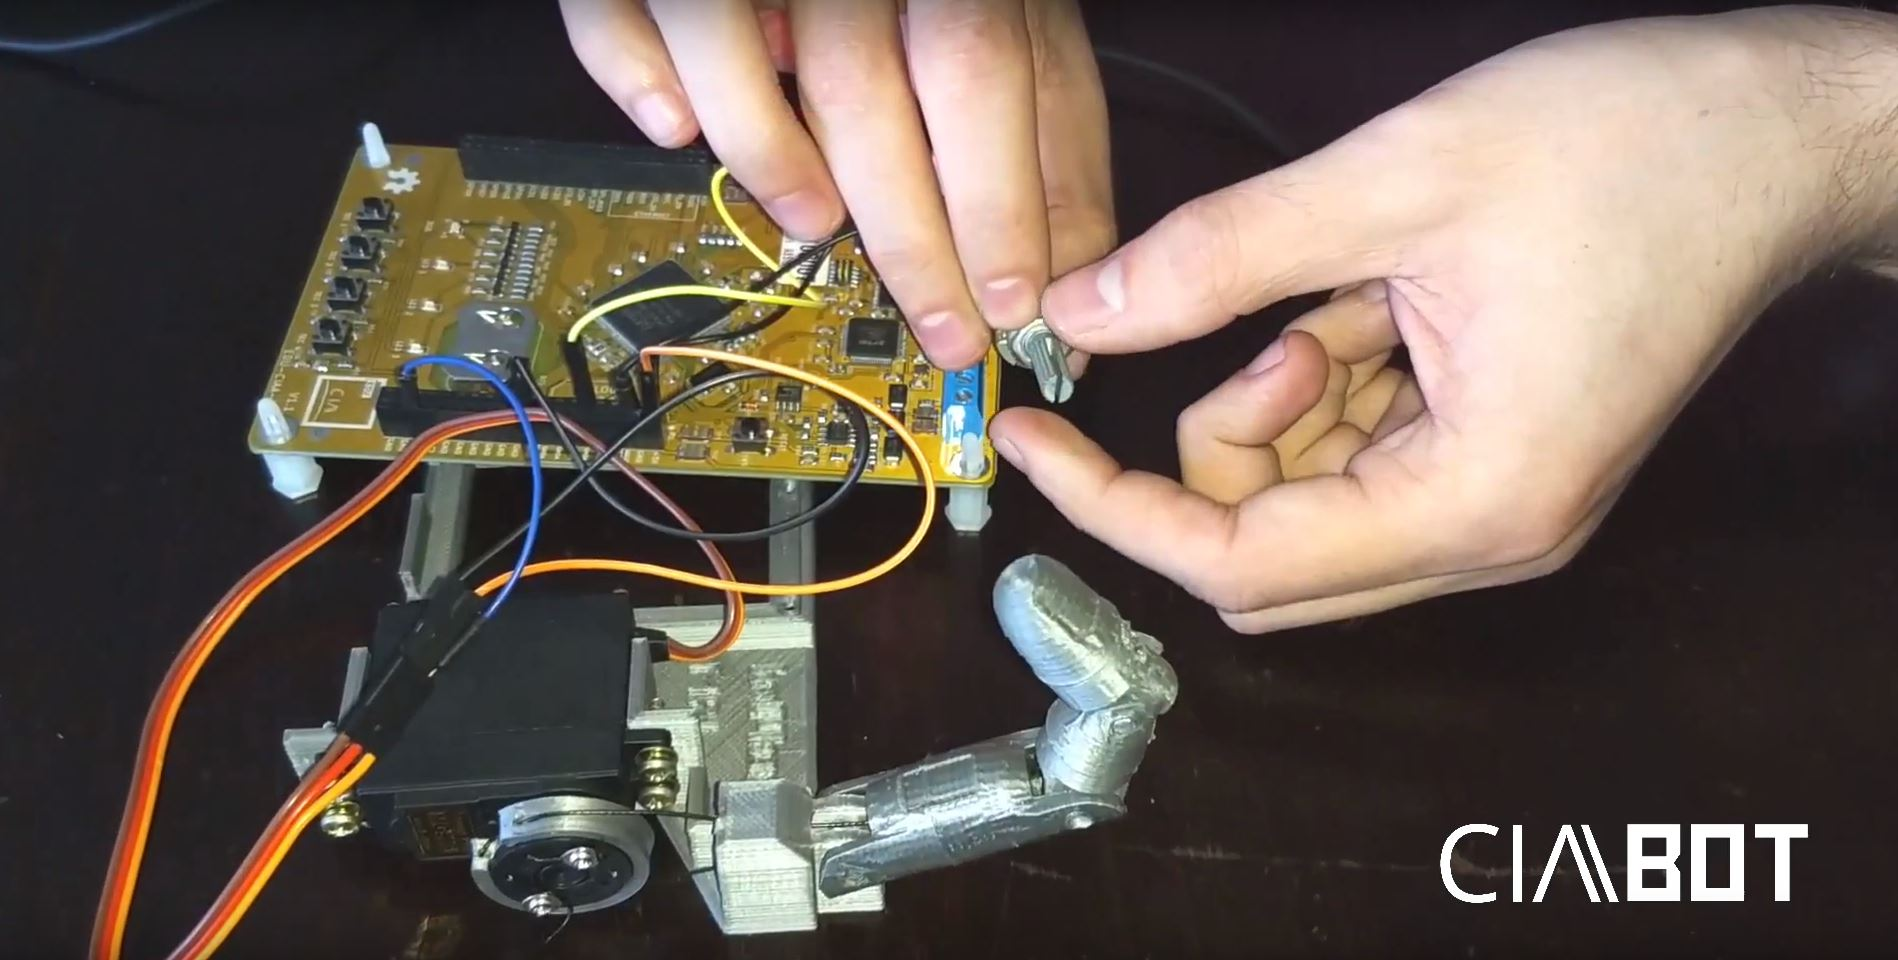
\includegraphics[scale=.3]{./Figures/dedo-servo.jpg}
\caption{Prueba de servomotor sobre dedo 3D.}
\label{fig:dedoServo}
\end{figure}

Teniendo en mente la necesidad de desarrollar ejemplos didácticos para utilizar CIAABOT, se utilizaron materiales desarrollados y provistos por la Universidad Nacional de Quilmes, en el marco del proyecto "La universidad y la escuela secundaria", dirigido por Cristina Wainmaier (Vicedirectora del Dto. de CyT, UNQ). Estos materiales incluían una maqueta de manejo de barreras y semáforos e instrumentos meteorológicos.

Para la verificación del correcto manejo del tiempo por parte del programa, se utilizó un anemómetro. Este dispositivo, que puede apreciarse en la figura \ref{fig:anemometro}, gira ante la presencia de viento y genera pulsos a intervalos angulares fijos. Conociendo la frecuencia de estos pulsos es posible determinar la velocidad del viento en cada momento.

Además, en este ensayo se probó la UART, proveyendo de una salida de consola por puerto serie, que podía observarse desde la PC. De esta manera el programa podía informar las mediciones realizadas, y guardarse en un archivo de log.

\begin{figure}[h]
\centering
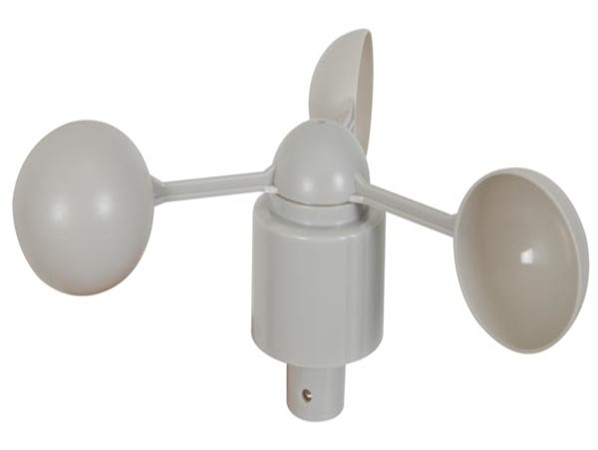
\includegraphics[scale=.8]{./Figures/anemometro.jpg}
\caption{Anemómetro utilizado en las pruebas.}
\label{fig:anemometro}
\end{figure}

De los instrumentos meteorológicos también se utilizó una rosa de los vientos formada por una matriz de leds. Con esto se validó el funcionamiento de las salidas digitales funcionando a la vez. En la figura \ref{fig:rosaVientos}, se observa un dibujo de la rosa de los vientos utilizada, así como la conexión de la matriz de leds que posee para encender los diferentes puntos cardinales.

\begin{figure}[H]
\centering
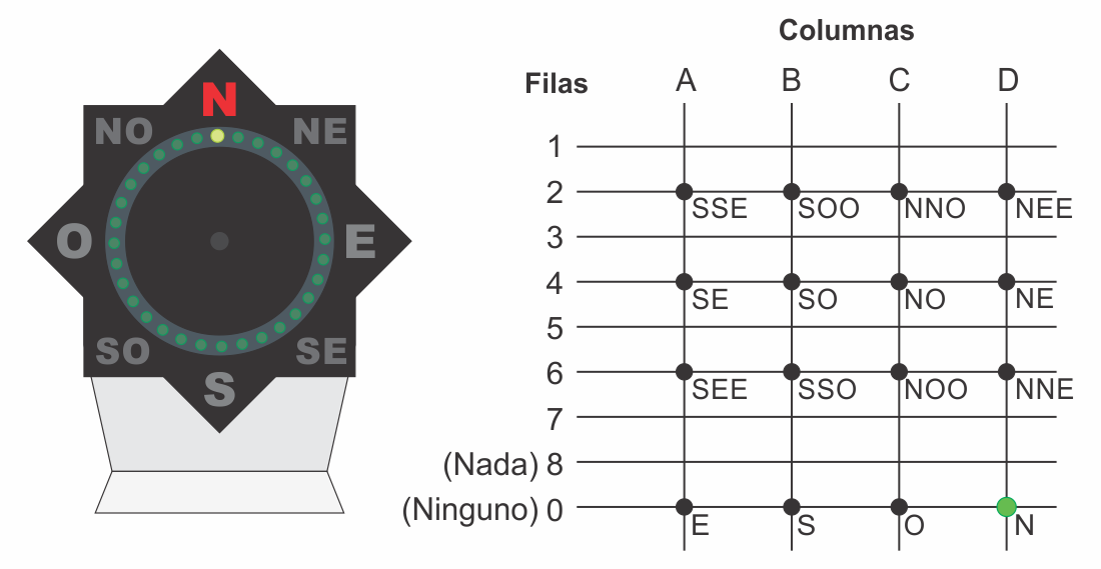
\includegraphics[scale=.6]{./Figures/rosa-vientos.png}
\caption{Rosa de los vientos y conexión de los leds.}
\label{fig:rosaVientos}
\end{figure}

\section{Workshop en el SASE}
Desde el 2010 se viene realizando año a año el Simposio Argentino de Sistemas Embebidos. Este evento es organizado por ACSE (Asociación Civil para la Investigación Promoción y Desarrollo de los Sistemas Electrónicos Embebidos). Es un evento anual que reúne a la comunidad académica y a la industria  en torno a esta temática, donde se realizan Tutoriales, Workshops y el Congreso Argentino de Sistemas Embebidos. 

En la edición de este año se agregó el workshop "Introducción a la programación de sistemas embebidos utilizando CIAABOT", que tuve la posibilidad de dictar y organizar en conjunto con el Ing. Eric Pernía. Estuvo orientado principalmente a alumnos de escuelas secundarias o entusiastas que buscaran una introducción a la programación de embebidos pero que no tuvieran conocimientos de ningún lenguaje para hacerlo.

Con una buena concurrencia se desarrolló la primera experiencia real en campo de la utilización de la plataforma CIAABOT para la enseñanza de programación. Se abarcaron temas básicos como el funcionamiento de sentencias condicionales, estructuras de control, lógica booleana y manejo básico de periféricos.

El workshop se realizó utilizando solamente CIAABOT IDE como medio para programar las placas. Se hizo uso de los elementos meteorológicos y la maqueta vehicular descrita en la sección \ref{sec:pruebas}, que puede observarse en la figura \ref{fig:maqueta}. Fue una buena oportunidad para obtener devoluciones por parte de los primeros usuarios de prueba, que fueron los asistentes al curso. Encontraron la aplicación intuitiva y se desenvolvieron de manera natural. Hubo dos casos puntuales de personas que no habían programado nunca antes de asistir, y ambos pudieron completar satisfactoriamente los ejercicios propuestos.

\begin{figure}[H]
\centering
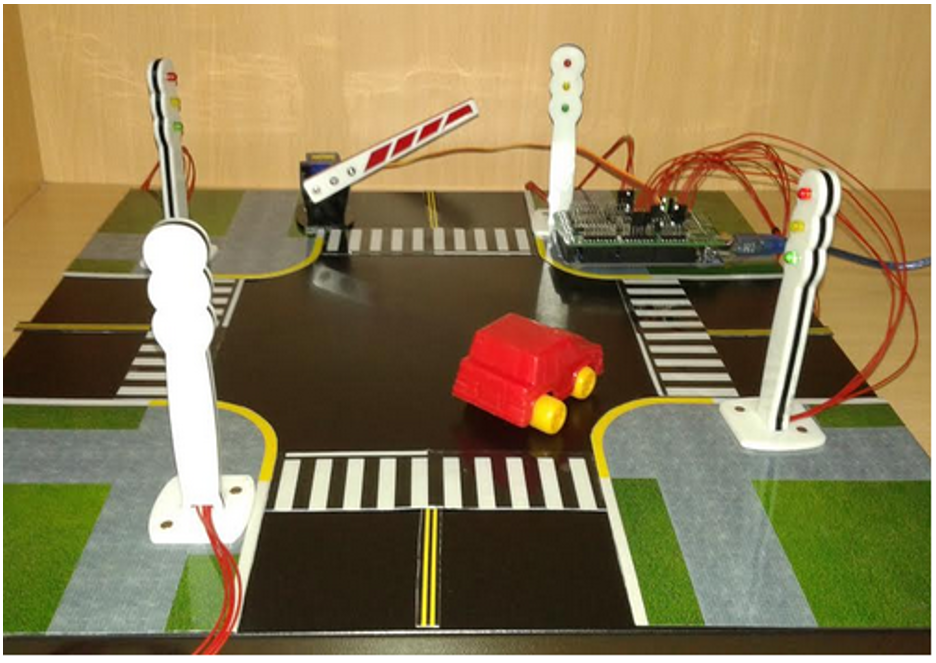
\includegraphics[scale=.8]{./Figures/maqueta.png}
\caption{Maqueta vehicular utilizada en el workshop.}
\label{fig:maqueta}
\end{figure}

\section{Experiencias en cursos CAPSE y de INET}
Los Cursos Abiertos de Programación de Sistemas Embebidos están orientados a personas con o sin experiencia previa, como docentes secundarios o universitarios, personal de empresas o estudiantes, que estén interesados en aprender a trabajar con sistemas embebidos. El objetivo de los cursos es aprender a realizar aplicaciones electrónicoas basadas en microcontroladores ARM de 32 bits, abordando desde problemas simples hasta problemas de mayor complejidad. Se utilizan kits compuestos por sensores y actuadores, y placas EDU-CIAA-NXP.

Además, cursos similares, y con objetivos alineados a los de los CAPSE, se brindaron a pedido del Instituto Nacional de Educación Tecnológica (INET).

En la última edición de estos cursos se utilizó CIAABOT IDE para las primeras clases, como manera de introducir a los asistentes a los conceptos básicos de la programación, así como también para obtener resultados rápidos. 

Esta segunda experiencia de uso de CIAABOT en un entorno real de enseñanza fue realmente útil. Se obtuvieron recomendaciones y se registraron errores descubiertos a raíz de casos de uso que no se tuvieron en cuenta a la hora del desarrollo. Todas estas mejoras y errores fueron registrados en la sección de \emph{issues} del repositorio de CIAABOT.

Por ejemplo, gran parte de los asistentes poseían netbooks con pantallas de resolución limitada, lo que hacía algo dificultoso el manejo de la vista partida que presenta el editor gráfico del IDE en conjunto con la salida del código C. Además, la sección de proyectos recientes y el formulario de 'Nuevo Proyecto' no se mostraban de manera cómoda. A raíz de esto, se comenzó un proceso de mejora de la adaptación de la aplicación ante cambios de resoluciones de pantalla, a lo que se refiere en inglés como  \emph{responsiveness}.

\section{Uso en un proyecto de brazo robótico}
El Laboratorio Abierto de la Universidad Tecnológica Nacional Facultad Regional Avellaneda, comenzó este año el desarrollo de una prótesis de brazo y mano robótica, impresas en 3D. La mano cuenta con movilidad en la muñeca y las falanges de los dedos, logrando así una funcionalidad similar a la de la mano humana. El brazo puede observarse en la figura \ref{fig:brazo}.

\begin{figure}[H]
\centering
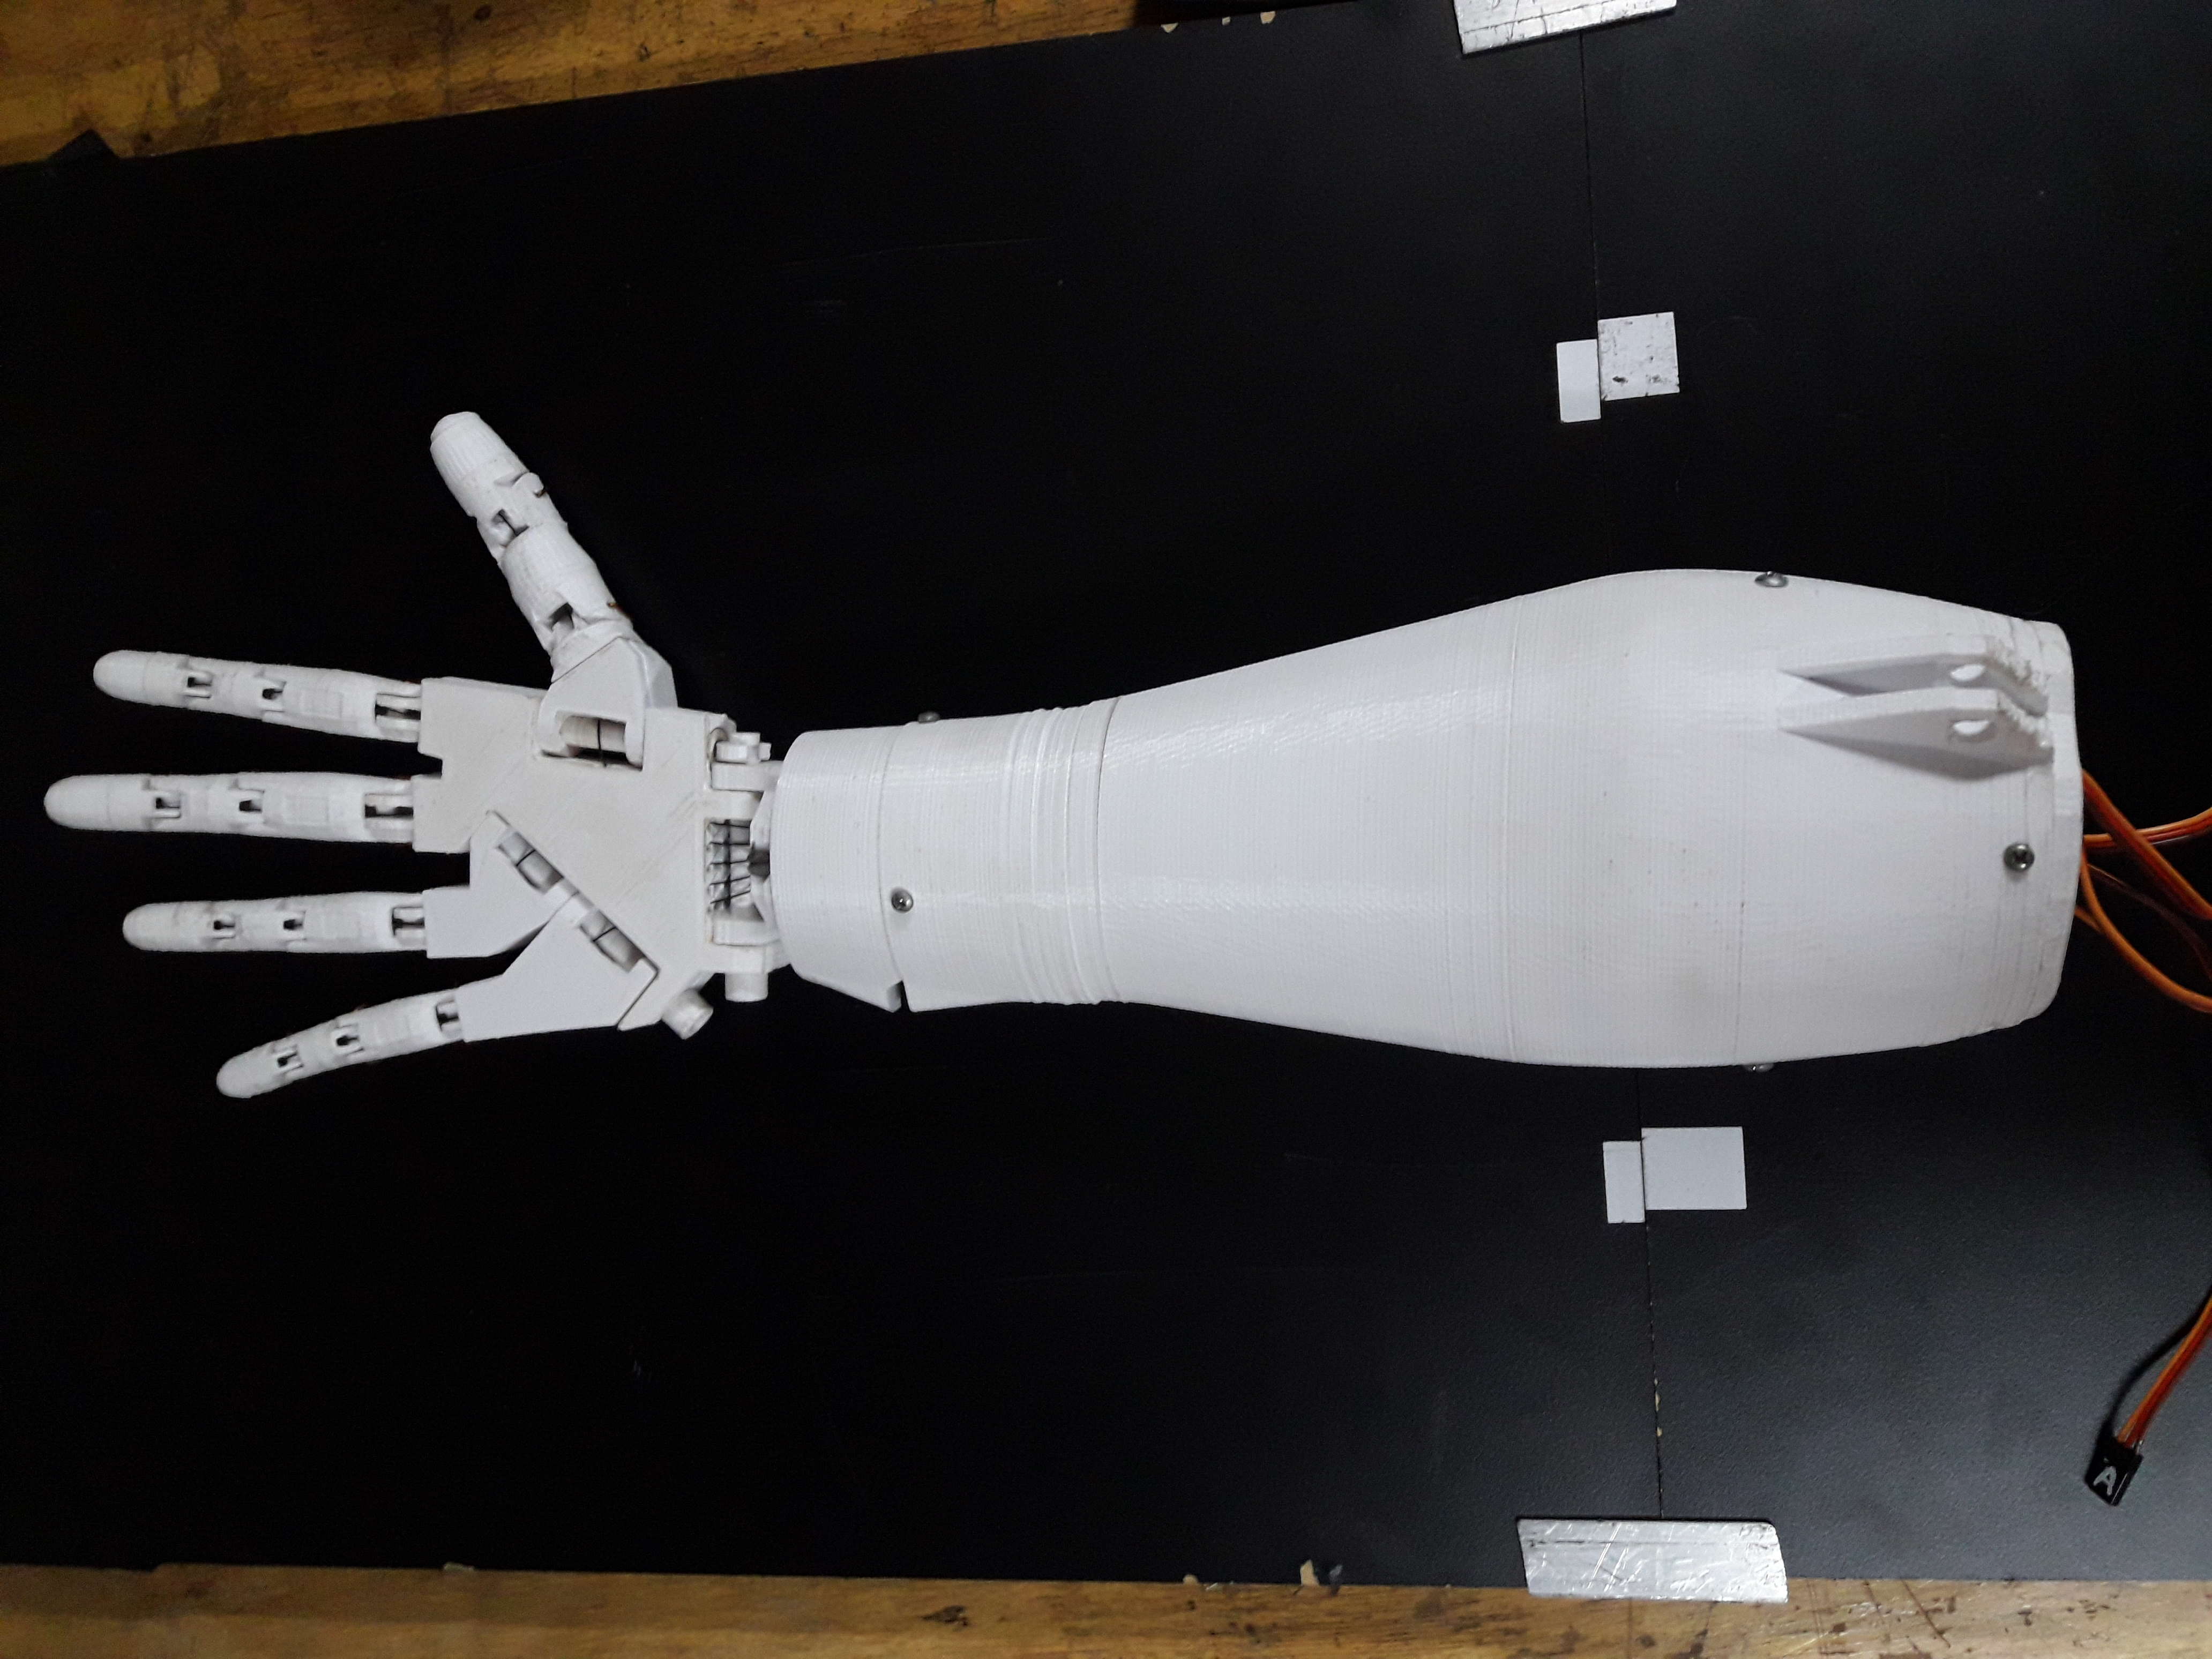
\includegraphics[scale=.1]{./Figures/brazo.jpg}
\caption{Prótesis impresa en 3D.}
\label{fig:brazo}
\end{figure}

El objetivo principal del mismo, es poder realizar un aporte a la mejora de la calidad de vida de personas con amputaciones parciales de brazo y mano. Se utilizan las señales bioeléctricas obtenidas superficialmente desde el músculo del usuario para luego transformarla en una señal eléctrica capaz de manipularse, con el fin de controlarla. Por tal motivo, el faltante de miembro del paciente no debe ser total, para permitir una colocación de 3 electrodos.

Actualmente el proyecto busca migrarse a microcontroladores de 32 bits, y se optó utilizar la placa EDU-CIAA-NXP. Esto es debido a que las mediciones de los electrodos sirven para realizar un control rudimentario y detectar si el músculo está contraído o no, pero no alcanza para obtener una señal proporcional a la fuerza ejercida para emular este movimiento en la prótesis.

La idea es mejorar algoritmo de detección de fuerza en el músculo, realizando un análisis en el dominio de la frecuencia con el objetivo de eliminar ruidos propios que se generan por el tipo de contacto que tienen los sensores. Para esto, se pretende hacer uso de la unidad de punto flotante presente en el LPC4337. Para las primeras pruebas de manejo de hardware y lectura de los sensores musculares, se utilizaron programas armados en CIAABOT IDE.
 
	% Chapter Template

\chapter{Conclusiones} % Main chapter title

\label{Chapter5} % Change X to a consecutive number; for referencing this chapter elsewhere, use \ref{ChapterX}


%----------------------------------------------------------------------------------------

%----------------------------------------------------------------------------------------
%	SECTION 1
%----------------------------------------------------------------------------------------

\section{Conclusiones generales }

La idea de esta sección es resaltar cuáles son los principales aportes del trabajo realizado y cómo se podría continuar. Debe ser especialmente breve y concisa. Es buena idea usar un listado para enumerar los logros obtenidos.

%----------------------------------------------------------------------------------------
%	SECTION 2
%----------------------------------------------------------------------------------------
\section{Próximos pasos}

Acá se indica cómo se podría continuar el trabajo más adelante.
 
\end{verbatim}

Los apéndices también deben ir en archivos .tex separados y se deben ubicar dentro de la carpeta \emph{Appendices}. Los apéndices vienen comentados con el caracter \code{\%} por defecto y para incluirlos se debe eliminar dicho caracter.

Luego del preambulo, los capítulos y los apéndices, finalmente viene la bibliografía. El estilo bibliográfico (llamado \option{authoryear}) es utilizado por \LaTeX{} para generar las referencias y es un estilo con todas las características necesarias para su composición.  No se debe subestimar lo agradecido que estarán sus lectores al encontrar que las referencias se encuentran a un clic de distancia.  Por supuesto, esto depende de que usted haya puesto la url correspondiente en el archivo BibTex en primer lugar.

%----------------------------------------------------------------------------------------







	\chapter{Introducción Específica} % Main chapter title

\label{Chapter2}
En este capítulo se presenta CIAABOT con más detalle, incluyendo especificaciones técnicas sobre la plataforma utilizada. Se establecen los requerimientos planteados y la planificación para el desarrollo del trabajo.

\section{CIAABOT: Partes componentes}
\label{sec:ciaabot:partes}
Se planteó que para lograr los objetivos propuestos, la plataforma debería estar formada por tres partes fundamentales, que funcionarían complementadas para armar un ecosistema CIAABOT, como está esquematizado en la figura \ref{fig:ciaabot:partes}. A continuación se describirá cada uno de ellos.

\begin{center}
    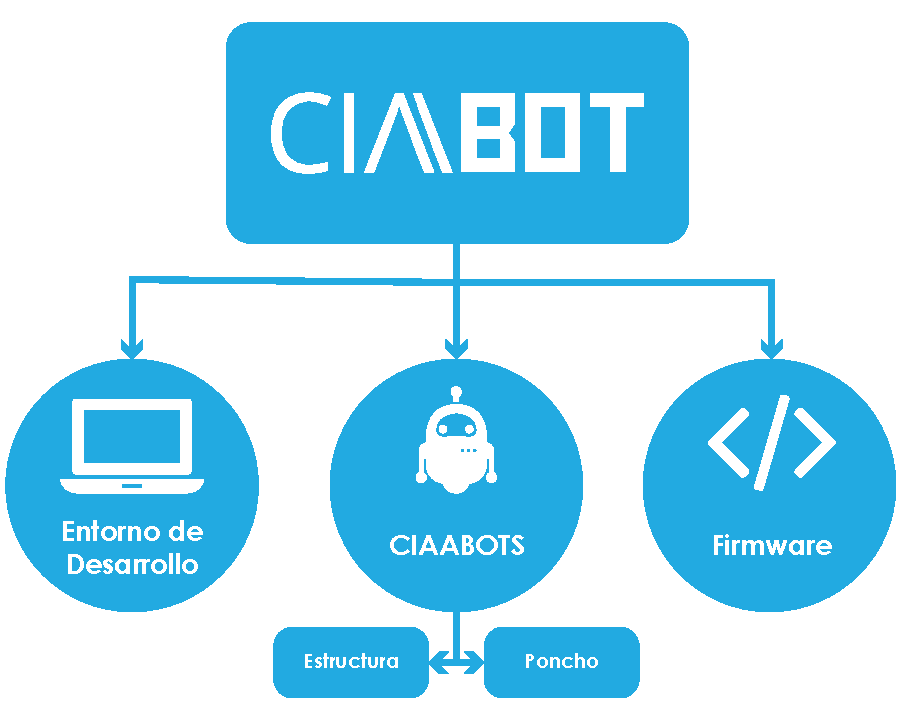
\includegraphics[scale=.8]{./Figures/ciaabot-partes.pdf}
    \label{fig:ciaabot:partes}
    \captionof{figure}{Diagrama de las partes que componen CIAABOT.}
\end{center}


\subsection{Entorno de desarrollo integrado}
\label{subsec:ide}
Un IDE (\emph{Integrated Development Environment}, Entorno de Desarrollo Integrado) es un software que incluye varias herramientas para asistir a los desarrolladores con su trabajo. Generalmente incluye algún editor para el código, herramientas de construcción o compilación automáticas, programación de la plataforma y posible depuración.

El CIAABOT-IDE es el centro del trabajo de los usuarios. Aquí plasman sus ideas y soluciones a problemas planteados. Esto lo hacen por medio de un editor de código en el que utilizan bloques predefinidos y no texto, como se observa en la figura \ref{fig:ciaabot:ide}. Arrastrando e interconectando los mismos logran definir la lógica para su programa.

Una opción interesante para remarcar es la salida de código en C. Cada vez que se modifica el diagrama de bloques, el código en C producido se modifica en tiempo real. Esto es muy útil para gente que pretende aprender a programar en C, ya que ve de manera directa cómo afecta cada bloque a las líneas de código y puede apreciar las equivalencias.

La plataforma también permite compilar y luego descargar el código generado en la placa solamente conectándola por USB.

Una vez que se finalizó el trabajo se puede guardar el proyecto en un archivo \emph{.cbp} que contiene la estructura de bloques en la que se estuvo trabajando, junto con las opciones adicionales del proyecto. Este archivo puede ser compartido y abierto en otra PC para ser reutilizado o modificado y guardado nuevamente.

Otra de las opciones que fue publicada en la última versión de CIAABOT-IDE (v0.0.8) es la de seleccionar los directorios de búsqueda para el toolchain. Las aplicaciones necesarias para todos los sistemas operativos son dos: El compilador arm-none-eabi-gcc y el debugger openOCD. Adicionalmente, en Windows se requieren otros ejecutables como make, para poder compilar y descargar el programa.

\begin{figure}[h]
	\centering
	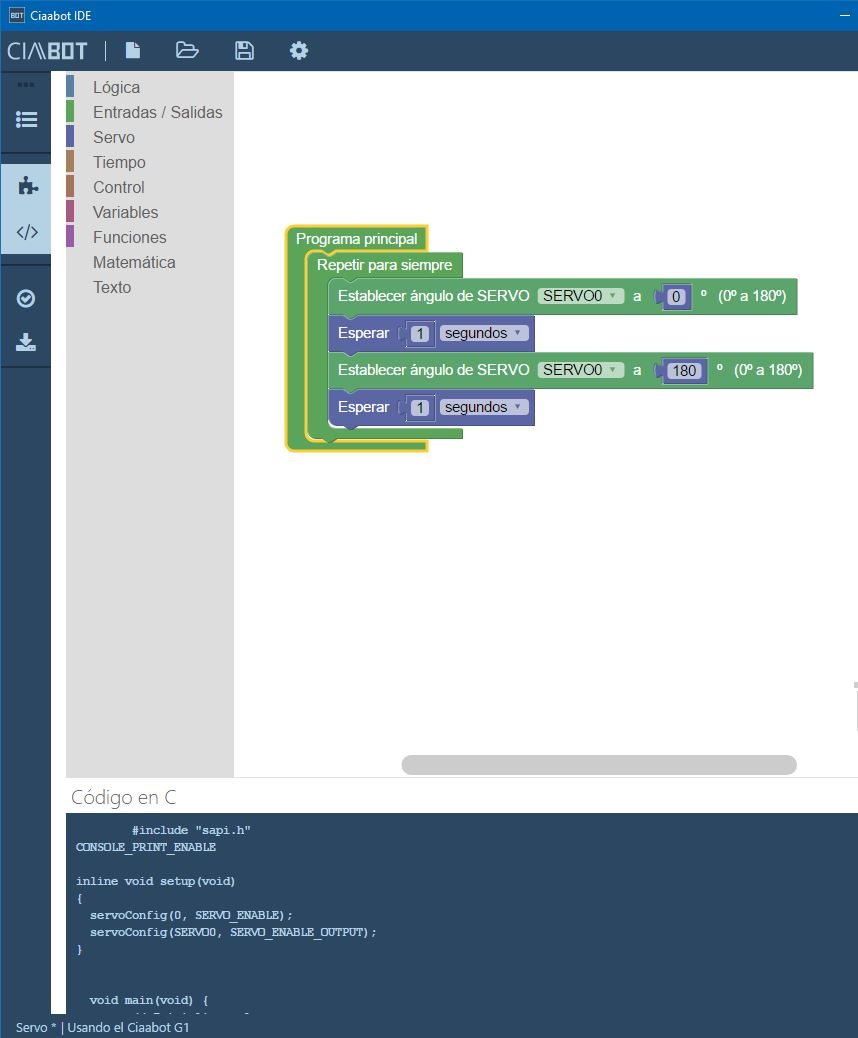
\includegraphics[scale=.5]{./Figures/ciaabot-ide-bloques.jpg}
	\caption{Editor gráfico de CIAABOT-IDE.}
	\label{fig:ciaabot:ide}
\end{figure}

\subsection{CIAABOTS}
\label{subsec:ciaabots}
Los robots que funcionen bajo esta plataforma serán denominados \emph{CIAABOTS}. Siguiendo la idea original de que CIAABOT sea utilizada en escuelas o por entusiastas, se planteó que estos robots estén diseñados estructuralmente para poder ser impresos con impresoras 3D.

De esta manera es posible enviar los archivos para imprimirlos en cualquier escuela que cuente con este sistema de impresión para replicarlo. Sólo sería necesario tener la placa CIAA correspondiente al modelo, armar el poncho (de diseño abierto) y adquirir en algún lugar de conveniencia los actuadores o sensores particulares del CIAABOT (motores DC, sensores IR, ultrasonido, etc.).

El diseño del poncho para el primer modelo de CIAABOT, el G1 se puede encontrar en github \citep{CIAABOT:G1}, realizado con el suite KiCad como todos los diseños relacionados al proyecto CIAA.

\subsection{Firmware}
\label{subsec:firmware}
CIAABOT utiliza como base para su firmware dos proyectos principales del ecosistema CIAA: Firmware v2 \citep{CIAA:firmwarev2} y sAPI \citep{sAPI}. En conjunto proveen una forma simplificada de programar las placas CIAA.

La sAPI es una HAL (\emph{Hardware Abstraction Layer}, Capa de Abstracción de Hardware) para los microcontroladores, que permite acceder de manera simple a varios de los diferentes periféricos.

Juntando varias funciones de la sAPI es posible armar funciones más complejas de mayor nivel para manejar características más específicas de cada modelo de CIAABOT.

Se prevé que con el avance del desarrollo de la plataforma cada modelo tendrá bloques específicos que estarán disponibles en el editor, cuando se lo seleccione a la hora de armar el proyecto en el IDE. Así, podrían armarse bloques que realicen por ejemplo una lectura de un sensor, que implicaría el manejo de pines y tiempos de espera.

\section{Plataforma utilizada}
\label{sec:plataforma}
Como base para el proyecto se optó por utilizar CIAA. Es un proyecto centrado en el trabajo colaborativo que busca la innovación para crear, diseñar y desarrollar soluciones electrónicas en la industria. Dentro de sus objetivos se encuentran:

\begin{itemize}
\item Impulsar el desarrollo tecnológico nacional, a partir de sumar valor agregado al trabajo y a los productos y servicios, mediante el uso de sistemas electrónicos, en el marco de la vinculación de las instituciones educativas y el sistema científico-tecnológico con la industria.

\item Darle visibilidad positiva a la electrónica argentina.

\item Generar cambios estructurales en la forma en la que se desarrollan y utilizan en nuestro país los conocimientos en el ámbito de la electrónica y de las instituciones y empresas que hacen uso de ella. \citep{CIAA:wiki}
\end{itemize}

Se utiliza esta plataforma por compartir la misma idea de ser un proyecto libre, poseer una creciente comunidad e incentivar la industria nacional. Se consideró que es un proyecto suficientemente maduro y con actualizaciones y desarrollos constantes como para ser utilizado de base.

\subsection{EDU-CIAA-NXP}
\label{subsec:eduCiaaNxp}
La EDU-CIAA-NXP es la versión educativa y de bajo costo de la CIAA-NXP. Utiliza, al igual que la CIAA-NXP, el microcontrolador LPC4337 de NXP, un doble núcleo ARM Cortex-M4F y Cortex M0. Como se observa en la figura \ref{fig:eduCiaaNxp}, la placa posee 4 leds y 4 pulsadores de hardware adicional. Para ampliar sus capacidades se utilizan los conectores laterales, para adicionar alguna placa extensora llamada \emph{Poncho}.

\begin{figure}[h]
\centering
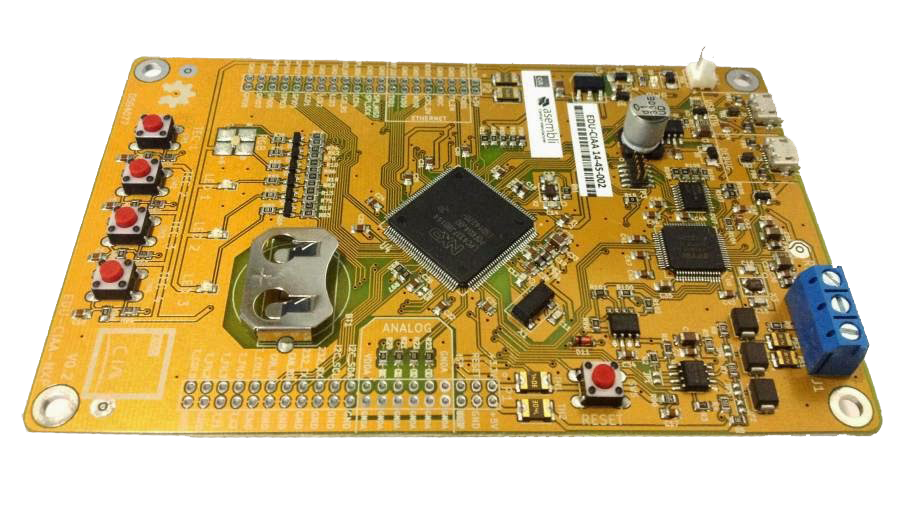
\includegraphics[scale=.5]{./Figures/edu-ciaa-nxp.png}
\caption{Placa EDU-CIAA-NXP}
\label{fig:eduCiaaNxp}
\end{figure}

Permite realizar programación y debugging, así como también acceder a una de sus UARTs, por medio de USB. Además posee otro puerto para que la placa funcione en modo OTG (\emph{On The Go}).

\section{Requerimientos}
\label{sec:requerimientos}
Se plantearon requerimientos que el proyecto debería cumplir a la hora de ser entregado. Se evaluaron sus posibilidades y se clasificaron en categorías.

\subsection{Requerimientos del sistema}
\label{subsec:requerimientosSistema}
Se estableció que el IDE debería poder ejecutarse como mínimo en un entorno Linux o Windows. Por la orientación didáctica del proyecto su uso debería ser simple, amigable y didáctico. Además, la programación debería poder realizarse íntegramente de manera gráfica por medio de bloques, donde cada uno represente acciones simples.

El IDE debería permitir un manejo de proyectos en forma de archivos, que posibilitaran el guardado y distribución de los mismos. Dentro de las opciones del proyecto debería poder seleccionarse el modelo de CIAABOT utilizado. Actualmente la opción existe, pero hay un solo modelo disponible.

El algoritmo que se genera a partir de los bloques debería estar disponible en lenguaje C, poder compilarse y programarse desde la aplicación, por puerto USB.

\subsection{Componentes del Sistema}
\label{subsec:componentesSistema}
Como ya se mencionó, se debería utilizar en principio la placa EDU-CIAA-NXP, y un poncho si fuese necesario para controlar la maqueta o robot implementado para la muestra. En el diseño de este poncho todos los periféricos deberían funcionar independientes al resto.

\subsection{Firmware}
\label{subsec:firmware}
Para el desarrollo del software se implementaría un sistema de control de versiones. Para la programación de los robots se utilizarían dos bibliotecas: En C la mencionada sAPI, y una de Firmata para un monitoreo del mismo por medio del puerto serie, con un cliente corriendo en la placa.

\subsection{Procesos Finales}
\label{subsec:procesosFinales}
Se requiere un manual de uso e instalación, junto con ejemplos básicos y funcionales, que sean representativos de las características de la plataforma. Se implementaría sobre una maqueta o robot adaptado a la EDU-CIAA, y con ello se evaluarían los resultados del proyecto y su aplicación en ámbitos de enseñanza reales.

\section{Planificación}
\label{sec:planificacion}
\subsection{Desglose en tareas}
En primer lugar, para definir objetivos concretos, se planteó una serie de entregables para el proyecto:

\begin{itemize}
\item IDE en funcionamiento.
\item Poncho CIAABOT G1 diseñado enteramente.
\item Manual de uso, instalación y ejemplos funcionales.
\item El presente informe final.
\end{itemize}

Siguiendo los lineamientos de las estrategias vistas en la materia Gestión de Proyectos, se procedió al diseño de una lista de desglose del trabajo en tareas. Se estimó un tiempo aproximado de 615 horas, distribuidas en grupos de tareas de la siguiente manera:

\begin{itemize}
\item Planificación del proyecto (40 hs.).
\item Investigación preliminar (45 hs.).
\item Selección de bibliotecas y plataformas (30 hs.).
\item Desarrollo de la aplicación de escritorio (45 hs.).
\item Desarrollo del editor gráfico (55 hs.).
\item Programación por USB y monitoreo (60 hs.).
\item Desarrollo del hardware (100 hs.).
\item Desarrollo del firmware (70 hs.).
\item Integración del sistema (50 hs.).
\item Procesos finales (120 hs.).
\end{itemize}
 
	\chapter{Diseño e Implementación} % Main chapter title

\label{Chapter3} % Change X to a consecutive number; for referencing this chapter elsewhere, use \ref{ChapterX}
\definecolor{mygreen}{rgb}{0,0.6,0}
\definecolor{mygray}{rgb}{0.5,0.5,0.5}
\definecolor{mymauve}{rgb}{0.58,0,0.82}

\lstset{ %
  backgroundcolor=\color{white},   % choose the background color; you must add \usepackage{color} or \usepackage{xcolor}
  basicstyle=\footnotesize,        % the size of the fonts that are used for the code
  breakatwhitespace=false,         % sets if automatic breaks should only happen at whitespace
  breaklines=true,                 % sets automatic line breaking
  captionpos=b,                    % sets the caption-position to bottom
  commentstyle=\color{mygreen},    % comment style
  deletekeywords={...},            % if you want to delete keywords from the given language
  %escapeinside={\%*}{*)},          % if you want to add LaTeX within your code
  %extendedchars=true,              % lets you use non-ASCII characters; for 8-bits encodings only, does not work with UTF-8
  %frame=single,	                   % adds a frame around the code
  keepspaces=true,                 % keeps spaces in text, useful for keeping indentation of code (possibly needs columns=flexible)
  keywordstyle=\color{blue},       % keyword style
  language=[ANSI]C,					% the language of the code
  %otherkeywords={*,...},           % if you want to add more keywords to the set
  numbers=left,                    % where to put the line-numbers; possible values are (none, left, right)
  numbersep=5pt,                   % how far the line-numbers are from the code
  numberstyle=\tiny\color{mygray}, % the style that is used for the line-numbers
  rulecolor=\color{black},         % if not set, the frame-color may be changed on line-breaks within not-black text (e.g. comments (green here))
  showspaces=false,                % show spaces everywhere adding particular underscores; it overrides 'showstringspaces'
  showstringspaces=false,          % underline spaces within strings only
  showtabs=false,                  % show tabs within strings adding particular underscores
  stepnumber=1,                    % the step between two line-numbers. If it's 1, each line will be numbered
  stringstyle=\color{mymauve},     % string literal style
  tabsize=2,	                   % sets default tabsize to 2 spaces
  title=\lstname,                   % show the filename of files included with \lstinputlisting; also try caption instead of title
  morecomment=[s]{/*}{*/}%
}


%----------------------------------------------------------------------------------------
%	SECTION 1
%----------------------------------------------------------------------------------------
\section{Estructura del Software}

sAPI
\begin{itemize}
\item Interrupciones.
\item SysTick.
\item GPIO.
\item UART.
\item ADC.
\item DAC.
\item $I^2C$.
\item SPI.
\item RTC.
\item SCT.
\item Timers.
\end{itemize}

Además incluye funciones avanzadas de conversión de datos, impresión formateada por UART, manejo de displays 7 segmentos, teclados matriciales, servos y PWM entre otras.

%----------------------------------------------------------------------------------------
La idea de esta sección es resaltar los problemas encontrados, los criterios utilizados y la justificación de las decisiones que se hayan tomado.

Se puede agregar código o pseudocódigo dentro de un entorno lstlisting con el siguiente código:

\begin{verbatim}
\begin{lstlisting}[caption= "un epígrafe descriptivo"]

	las líneas de código irían aquí...
	
\end{lstlisting}
\end{verbatim}

A modo de ejemplo:

\begin{lstlisting}[caption=Pseudocódigo del lazo principal de control.]  % Start your code-block

#define MAX_SENSOR_NUMBER 3
#define MAX_ALARM_NUMBER  6
#define MAX_ACTUATOR_NUMBER 6

uint32_t sensorValue[MAX_SENSOR_NUMBER];		
FunctionalState alarmControl[MAX_ALARM_NUMBER];	//ENABLE or DISABLE
state_t alarmState[MAX_ALARM_NUMBER];						//ON or OFF
state_t actuatorState[MAX_ACTUATOR_NUMBER];			//ON or OFF

void vControl() {

	initGlobalVariables();
	
	period = 500 ms;
		
	while(1) {

		ticks = xTaskGetTickCount();
		
		updateSensors();
		
		updateAlarms();
		
		controlActuators();
		
		vTaskDelayUntil(&ticks, period);
	}
}
\end{lstlisting}




	% Chapter Template

\chapter{Ensayos y Resultados} % Main chapter title

\label{Chapter4} % Change X to a consecutive number; for referencing this chapter elsewhere, use \ref{ChapterX}

%----------------------------------------------------------------------------------------
%	SECTION 1
%----------------------------------------------------------------------------------------

Este capítulo describe las pruebas que se realizaron sobre la plataforma, así como también su utilización en una situación aúlica real para dictado de cursos.

\section{Pruebas de sensores y actuadores}
\label{sec:pruebas}
Una vez desarrollados todos los bloques propuestos para la primera versión de la definición del lenguaje de CIAABOT, se pasó a una etapa de pruebas, para verificar que el manejo de los diferentes periféricos fuera correcta.

La primera prueba fue sobre un modelo impreso en 3D de un dedo índice, que es flexionado por un mecanismo accionado por un servomotor. En la figura \ref{fig:dedoServo} se observa el ensayo. Adicionalmente, la prueba también evaluó el funcionamiento de la lectura del conversor analógico-digital. Para esto se conectó un potenciómetro al canal 1 de conversión, que era leído constantemente.

El valor obtenido por el conversor (rango de 0 a 1023) era mapeado luego al rango admitido por la función de posicionamiento del servomotor (0 a 180), y luego era enviado al bloque de manejo del ángulo.

\begin{figure}[h]
\centering
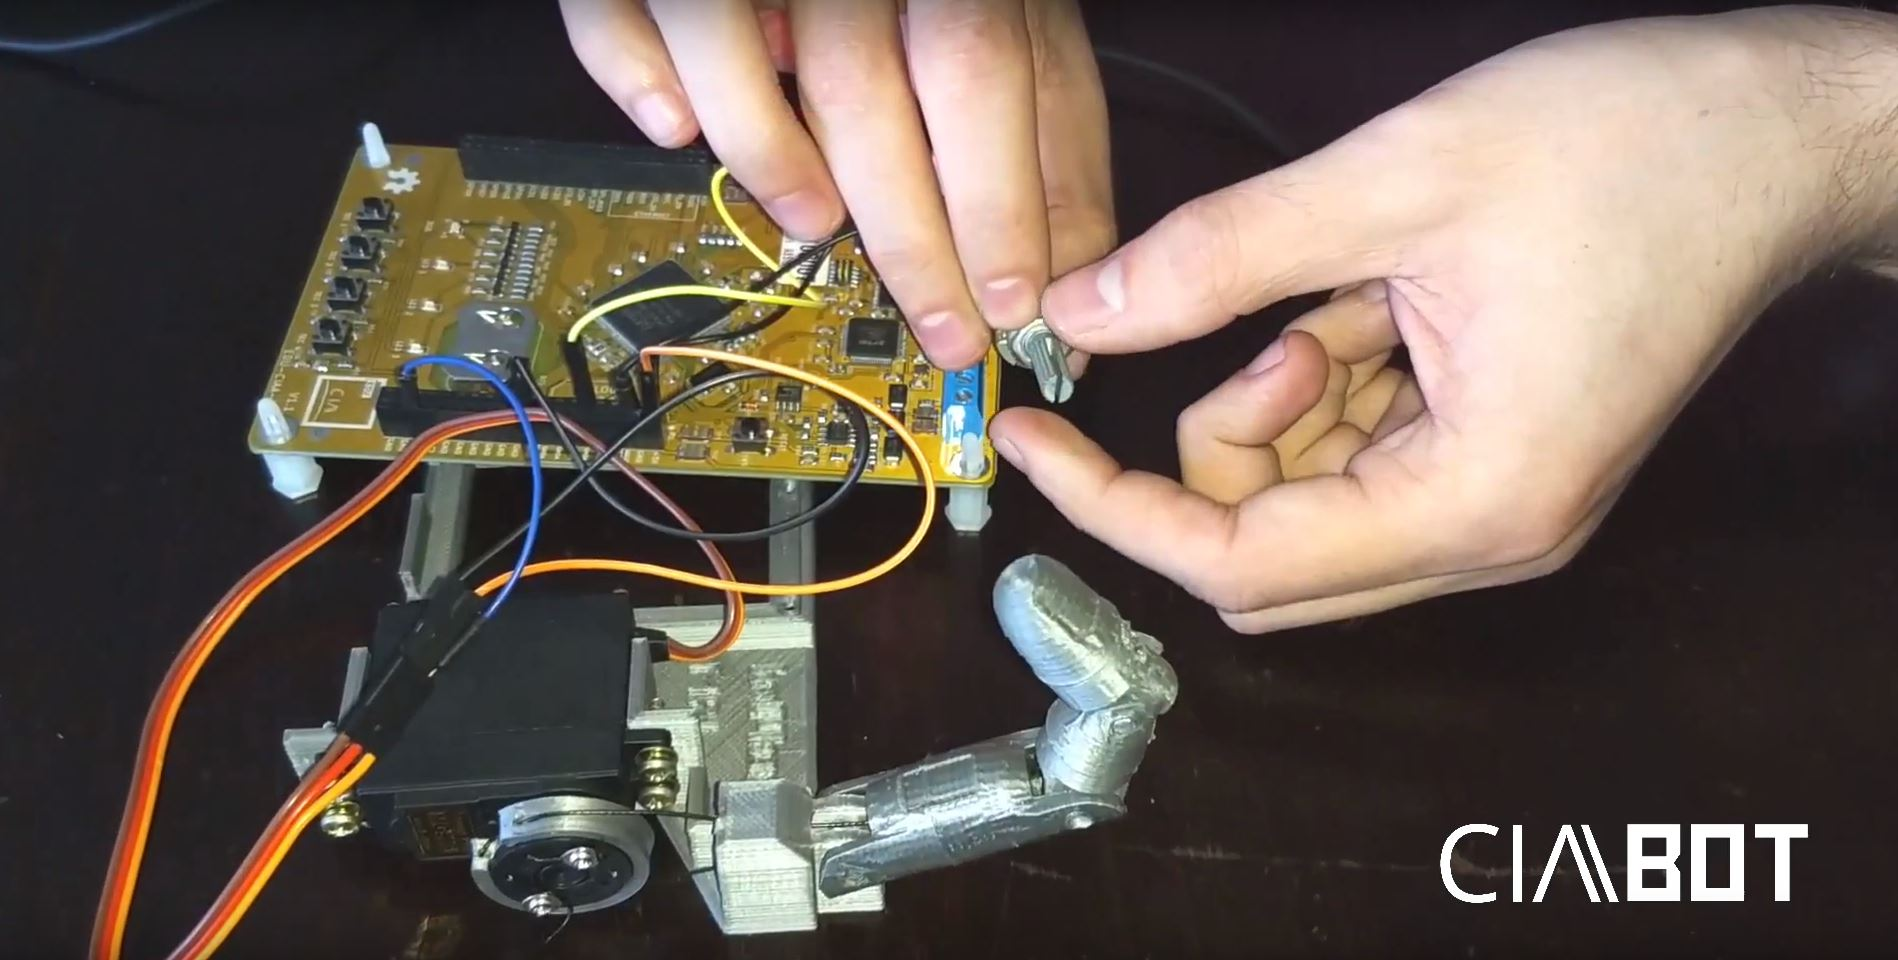
\includegraphics[scale=.3]{./Figures/dedo-servo.jpg}
\caption{Prueba de servomotor sobre dedo 3D.}
\label{fig:dedoServo}
\end{figure}

Teniendo en mente la necesidad de desarrollar ejemplos didácticos para utilizar CIAABOT, se utilizaron materiales desarrollados y provistos por la Universidad Nacional de Quilmes, en el marco del proyecto "La universidad y la escuela secundaria", dirigido por Cristina Wainmaier (Vicedirectora del Dto. de CyT, UNQ). Estos materiales incluían una maqueta de manejo de barreras y semáforos e instrumentos meteorológicos.

Para la verificación del correcto manejo del tiempo por parte del programa, se utilizó un anemómetro. Este dispositivo, que puede apreciarse en la figura \ref{fig:anemometro}, gira ante la presencia de viento y genera pulsos a intervalos angulares fijos. Conociendo la frecuencia de estos pulsos es posible determinar la velocidad del viento en cada momento.

Además, en este ensayo se probó la UART, proveyendo de una salida de consola por puerto serie, que podía observarse desde la PC. De esta manera el programa podía informar las mediciones realizadas, y guardarse en un archivo de log.

\begin{figure}[h]
\centering
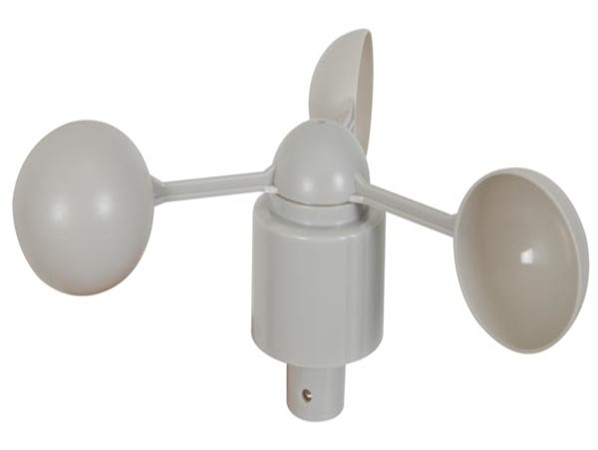
\includegraphics[scale=.8]{./Figures/anemometro.jpg}
\caption{Anemómetro utilizado en las pruebas.}
\label{fig:anemometro}
\end{figure}

De los instrumentos meteorológicos también se utilizó una rosa de los vientos formada por una matriz de leds. Con esto se validó el funcionamiento de las salidas digitales funcionando a la vez. En la figura \ref{fig:rosaVientos}, se observa un dibujo de la rosa de los vientos utilizada, así como la conexión de la matriz de leds que posee para encender los diferentes puntos cardinales.

\begin{figure}[H]
\centering
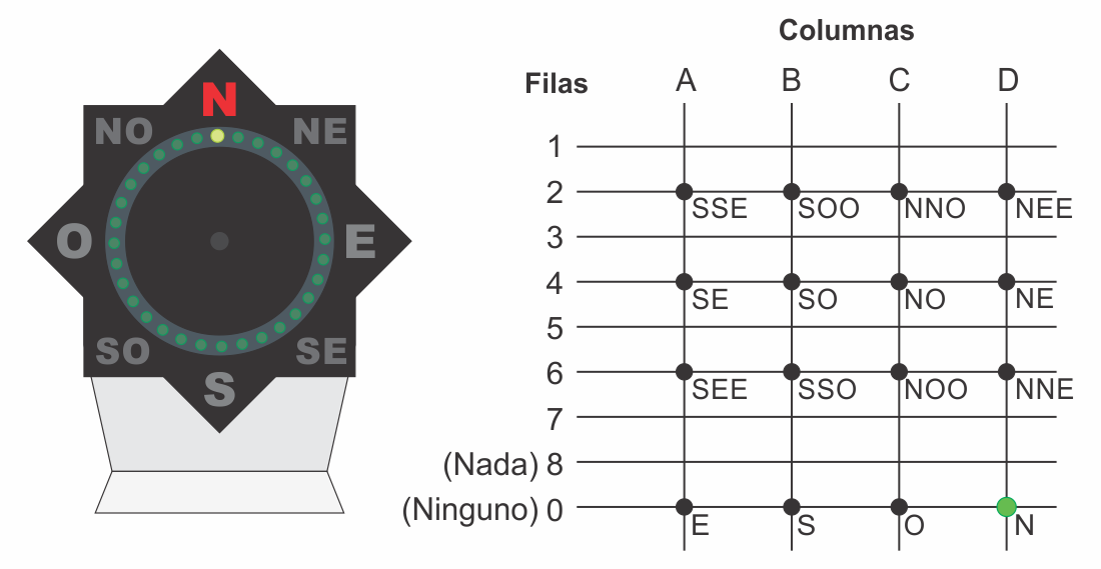
\includegraphics[scale=.6]{./Figures/rosa-vientos.png}
\caption{Rosa de los vientos y conexión de los leds.}
\label{fig:rosaVientos}
\end{figure}

\section{Workshop en el SASE}
Desde el 2010 se viene realizando año a año el Simposio Argentino de Sistemas Embebidos. Este evento es organizado por ACSE (Asociación Civil para la Investigación Promoción y Desarrollo de los Sistemas Electrónicos Embebidos). Es un evento anual que reúne a la comunidad académica y a la industria  en torno a esta temática, donde se realizan Tutoriales, Workshops y el Congreso Argentino de Sistemas Embebidos. 

En la edición de este año se agregó el workshop "Introducción a la programación de sistemas embebidos utilizando CIAABOT", que tuve la posibilidad de dictar y organizar en conjunto con el Ing. Eric Pernía. Estuvo orientado principalmente a alumnos de escuelas secundarias o entusiastas que buscaran una introducción a la programación de embebidos pero que no tuvieran conocimientos de ningún lenguaje para hacerlo.

Con una buena concurrencia se desarrolló la primera experiencia real en campo de la utilización de la plataforma CIAABOT para la enseñanza de programación. Se abarcaron temas básicos como el funcionamiento de sentencias condicionales, estructuras de control, lógica booleana y manejo básico de periféricos.

El workshop se realizó utilizando solamente CIAABOT IDE como medio para programar las placas. Se hizo uso de los elementos meteorológicos y la maqueta vehicular descrita en la sección \ref{sec:pruebas}, que puede observarse en la figura \ref{fig:maqueta}. Fue una buena oportunidad para obtener devoluciones por parte de los primeros usuarios de prueba, que fueron los asistentes al curso. Encontraron la aplicación intuitiva y se desenvolvieron de manera natural. Hubo dos casos puntuales de personas que no habían programado nunca antes de asistir, y ambos pudieron completar satisfactoriamente los ejercicios propuestos.

\begin{figure}[H]
\centering
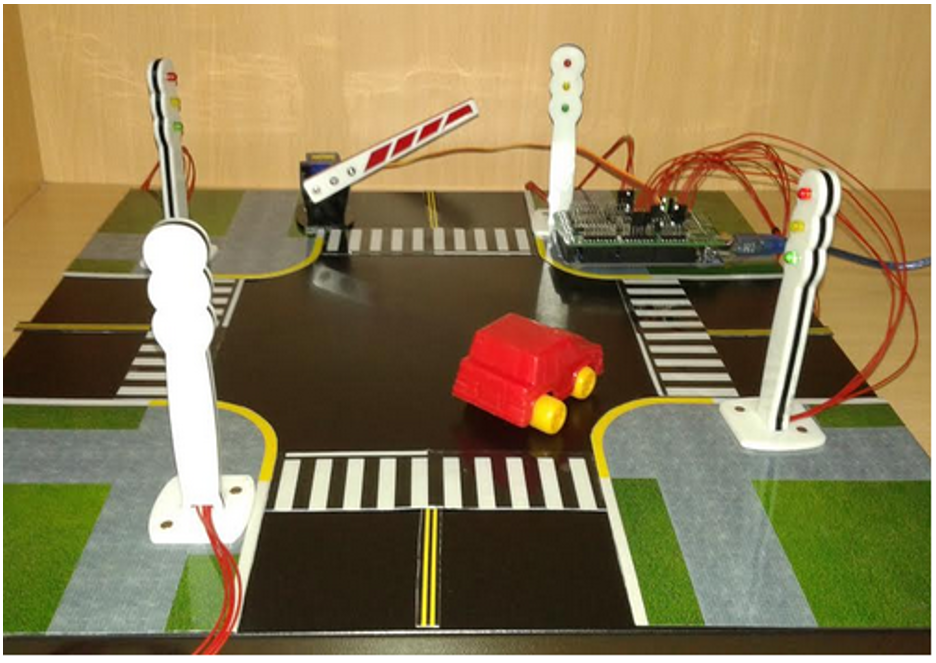
\includegraphics[scale=.8]{./Figures/maqueta.png}
\caption{Maqueta vehicular utilizada en el workshop.}
\label{fig:maqueta}
\end{figure}

\section{Experiencias en cursos CAPSE y de INET}
Los Cursos Abiertos de Programación de Sistemas Embebidos están orientados a personas con o sin experiencia previa, como docentes secundarios o universitarios, personal de empresas o estudiantes, que estén interesados en aprender a trabajar con sistemas embebidos. El objetivo de los cursos es aprender a realizar aplicaciones electrónicoas basadas en microcontroladores ARM de 32 bits, abordando desde problemas simples hasta problemas de mayor complejidad. Se utilizan kits compuestos por sensores y actuadores, y placas EDU-CIAA-NXP.

Además, cursos similares, y con objetivos alineados a los de los CAPSE, se brindaron a pedido del Instituto Nacional de Educación Tecnológica (INET).

En la última edición de estos cursos se utilizó CIAABOT IDE para las primeras clases, como manera de introducir a los asistentes a los conceptos básicos de la programación, así como también para obtener resultados rápidos. 

Esta segunda experiencia de uso de CIAABOT en un entorno real de enseñanza fue realmente útil. Se obtuvieron recomendaciones y se registraron errores descubiertos a raíz de casos de uso que no se tuvieron en cuenta a la hora del desarrollo. Todas estas mejoras y errores fueron registrados en la sección de \emph{issues} del repositorio de CIAABOT.

Por ejemplo, gran parte de los asistentes poseían netbooks con pantallas de resolución limitada, lo que hacía algo dificultoso el manejo de la vista partida que presenta el editor gráfico del IDE en conjunto con la salida del código C. Además, la sección de proyectos recientes y el formulario de 'Nuevo Proyecto' no se mostraban de manera cómoda. A raíz de esto, se comenzó un proceso de mejora de la adaptación de la aplicación ante cambios de resoluciones de pantalla, a lo que se refiere en inglés como  \emph{responsiveness}.

\section{Uso en un proyecto de brazo robótico}
El Laboratorio Abierto de la Universidad Tecnológica Nacional Facultad Regional Avellaneda, comenzó este año el desarrollo de una prótesis de brazo y mano robótica, impresas en 3D. La mano cuenta con movilidad en la muñeca y las falanges de los dedos, logrando así una funcionalidad similar a la de la mano humana. El brazo puede observarse en la figura \ref{fig:brazo}.

\begin{figure}[H]
\centering
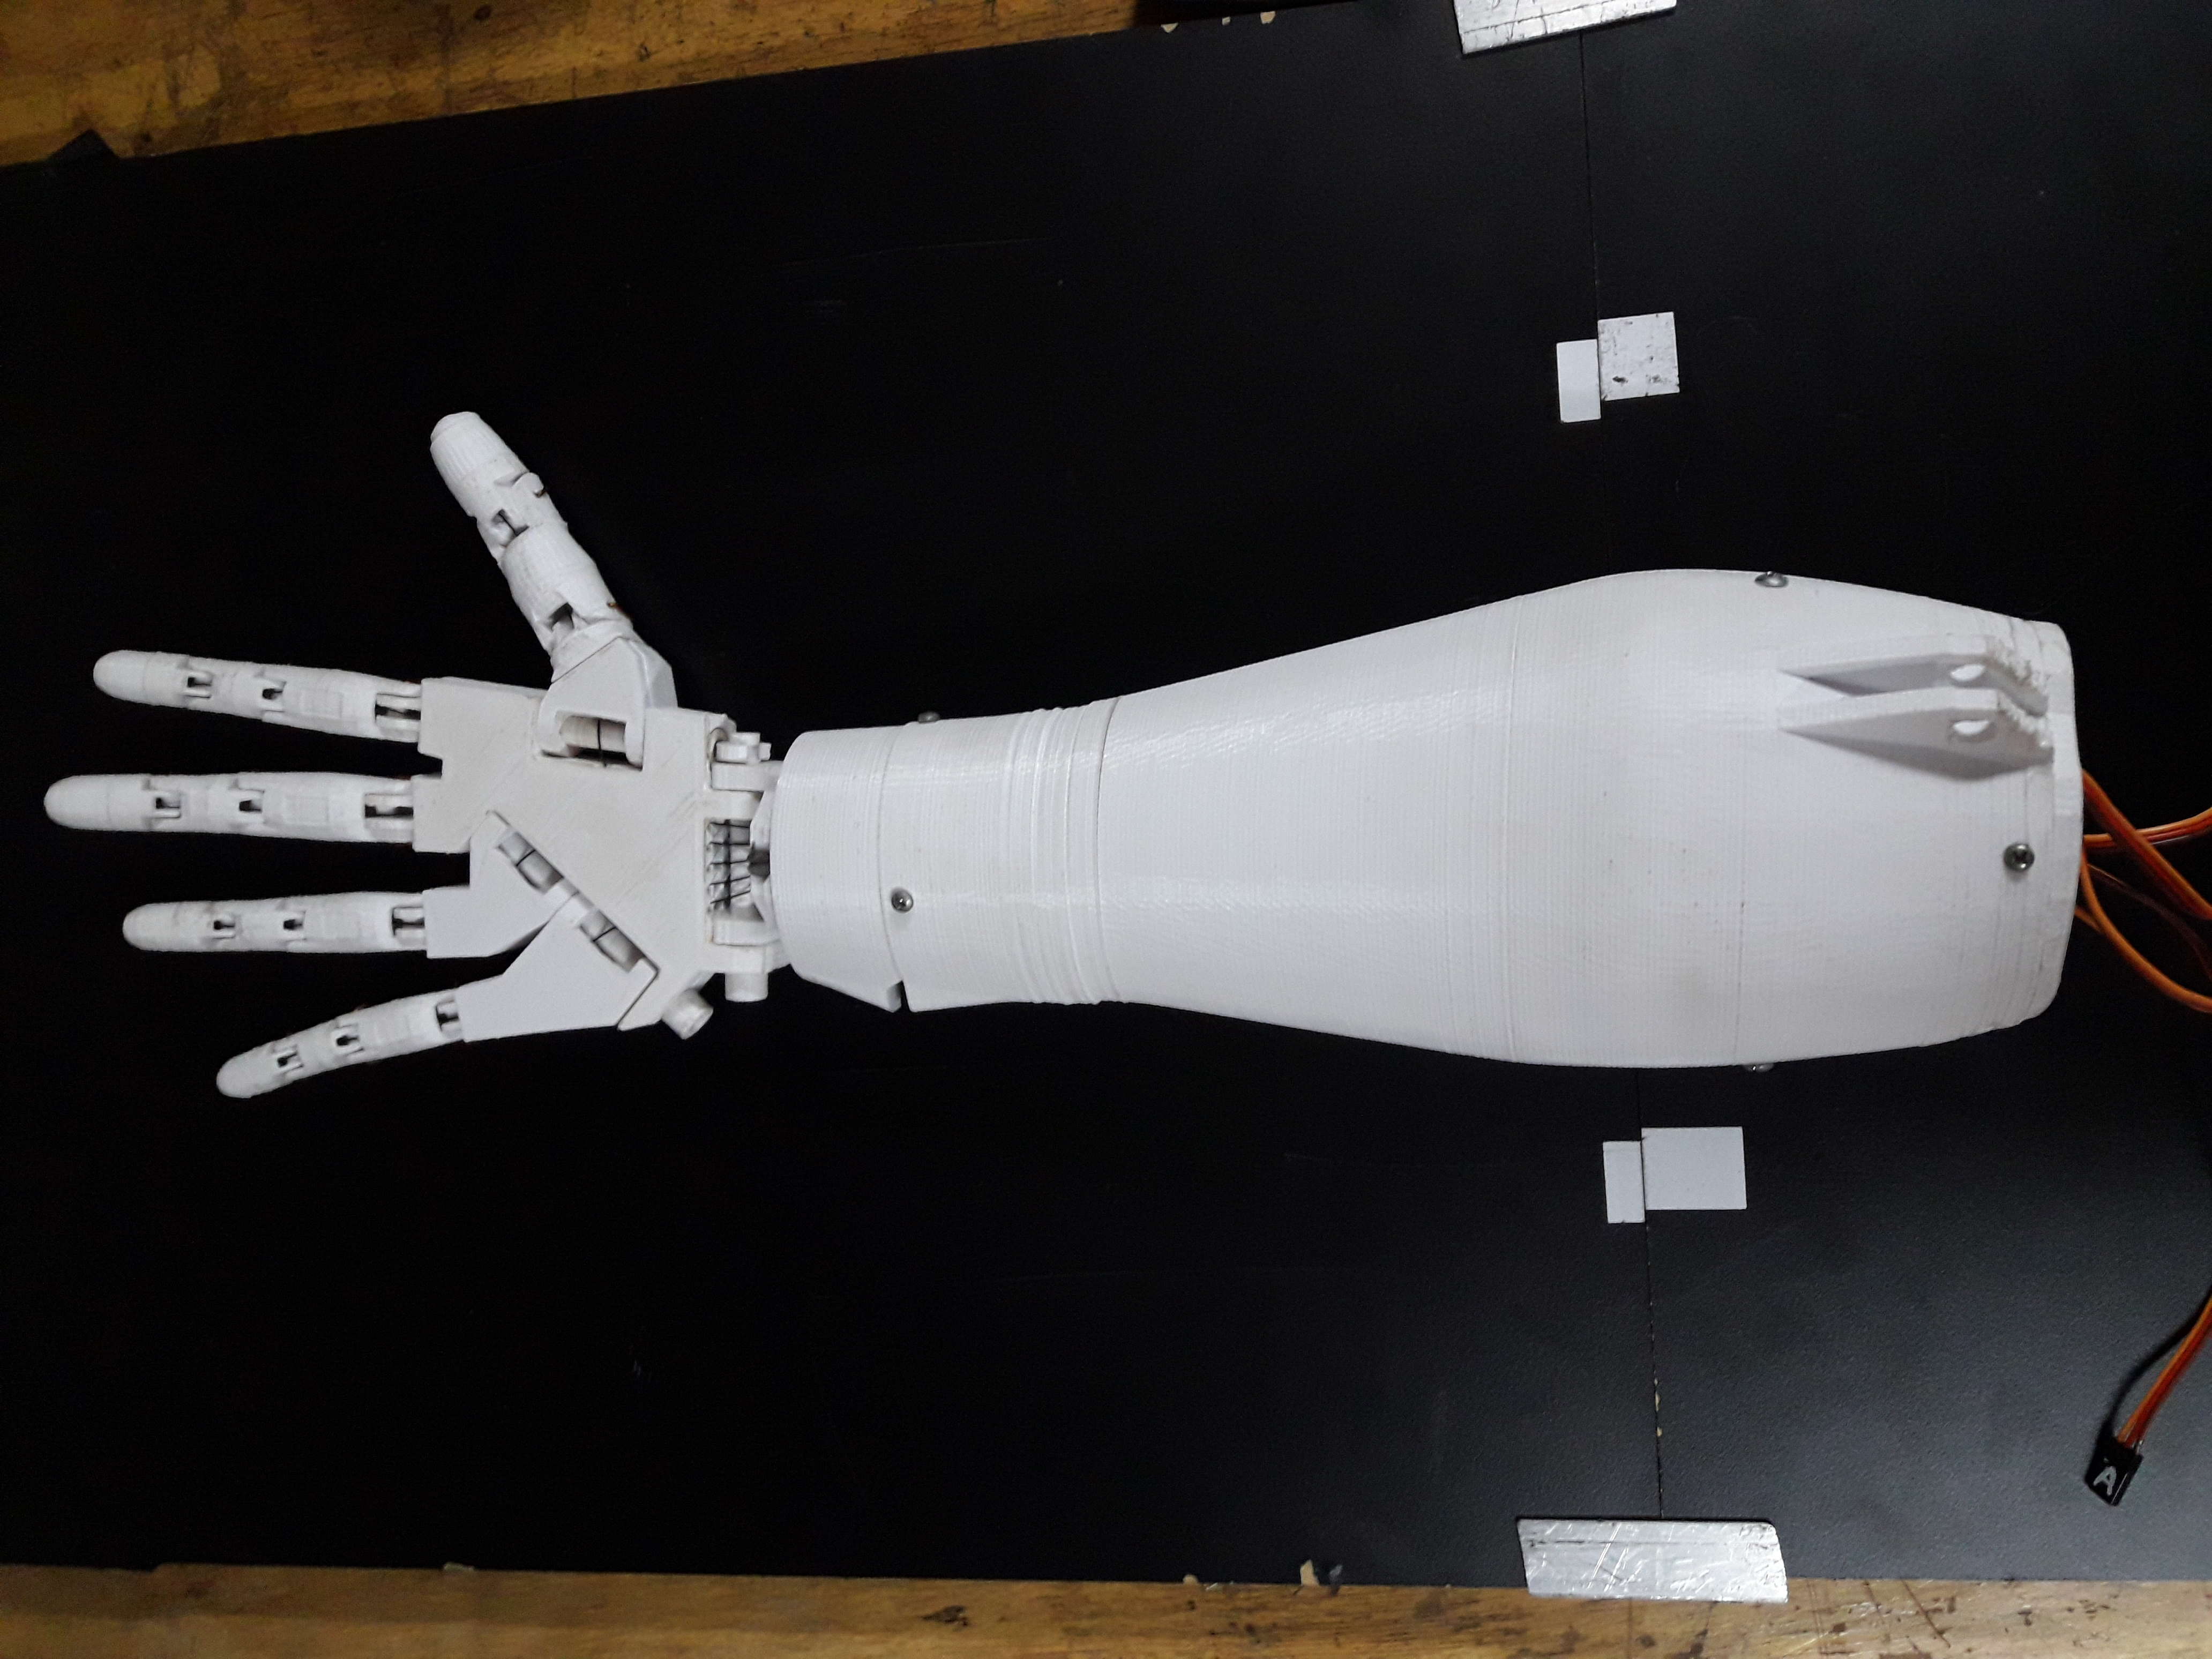
\includegraphics[scale=.1]{./Figures/brazo.jpg}
\caption{Prótesis impresa en 3D.}
\label{fig:brazo}
\end{figure}

El objetivo principal del mismo, es poder realizar un aporte a la mejora de la calidad de vida de personas con amputaciones parciales de brazo y mano. Se utilizan las señales bioeléctricas obtenidas superficialmente desde el músculo del usuario para luego transformarla en una señal eléctrica capaz de manipularse, con el fin de controlarla. Por tal motivo, el faltante de miembro del paciente no debe ser total, para permitir una colocación de 3 electrodos.

Actualmente el proyecto busca migrarse a microcontroladores de 32 bits, y se optó utilizar la placa EDU-CIAA-NXP. Esto es debido a que las mediciones de los electrodos sirven para realizar un control rudimentario y detectar si el músculo está contraído o no, pero no alcanza para obtener una señal proporcional a la fuerza ejercida para emular este movimiento en la prótesis.

La idea es mejorar algoritmo de detección de fuerza en el músculo, realizando un análisis en el dominio de la frecuencia con el objetivo de eliminar ruidos propios que se generan por el tipo de contacto que tienen los sensores. Para esto, se pretende hacer uso de la unidad de punto flotante presente en el LPC4337. Para las primeras pruebas de manejo de hardware y lectura de los sensores musculares, se utilizaron programas armados en CIAABOT IDE.
 
	% Chapter Template

\chapter{Conclusiones} % Main chapter title

\label{Chapter5} % Change X to a consecutive number; for referencing this chapter elsewhere, use \ref{ChapterX}


%----------------------------------------------------------------------------------------

%----------------------------------------------------------------------------------------
%	SECTION 1
%----------------------------------------------------------------------------------------

\section{Conclusiones generales }

La idea de esta sección es resaltar cuáles son los principales aportes del trabajo realizado y cómo se podría continuar. Debe ser especialmente breve y concisa. Es buena idea usar un listado para enumerar los logros obtenidos.

%----------------------------------------------------------------------------------------
%	SECTION 2
%----------------------------------------------------------------------------------------
\section{Próximos pasos}

Acá se indica cómo se podría continuar el trabajo más adelante.
 
\end{verbatim}

Los apéndices también deben ir en archivos .tex separados y se deben ubicar dentro de la carpeta \emph{Appendices}. Los apéndices vienen comentados con el caracter \code{\%} por defecto y para incluirlos se debe eliminar dicho caracter.

Luego del preambulo, los capítulos y los apéndices, finalmente viene la bibliografía. El estilo bibliográfico (llamado \option{authoryear}) es utilizado por \LaTeX{} para generar las referencias y es un estilo con todas las características necesarias para su composición.  No se debe subestimar lo agradecido que estarán sus lectores al encontrar que las referencias se encuentran a un clic de distancia.  Por supuesto, esto depende de que usted haya puesto la url correspondiente en el archivo BibTex en primer lugar.

%----------------------------------------------------------------------------------------







\chapter{Introducción Específica} % Main chapter title

\label{Chapter2}
En este capítulo se presenta CIAABOT con más detalle, incluyendo especificaciones técnicas sobre la plataforma utilizada. Se establecen los requerimientos planteados y la planificación para el desarrollo del trabajo.

\section{CIAABOT: Partes componentes}
\label{sec:ciaabot:partes}
Se planteó que para lograr los objetivos propuestos, la plataforma debería estar formada por tres partes fundamentales, que funcionarían complementadas para armar un ecosistema CIAABOT, como está esquematizado en la figura \ref{fig:ciaabot:partes}. A continuación se describirá cada uno de ellos.

\begin{center}
    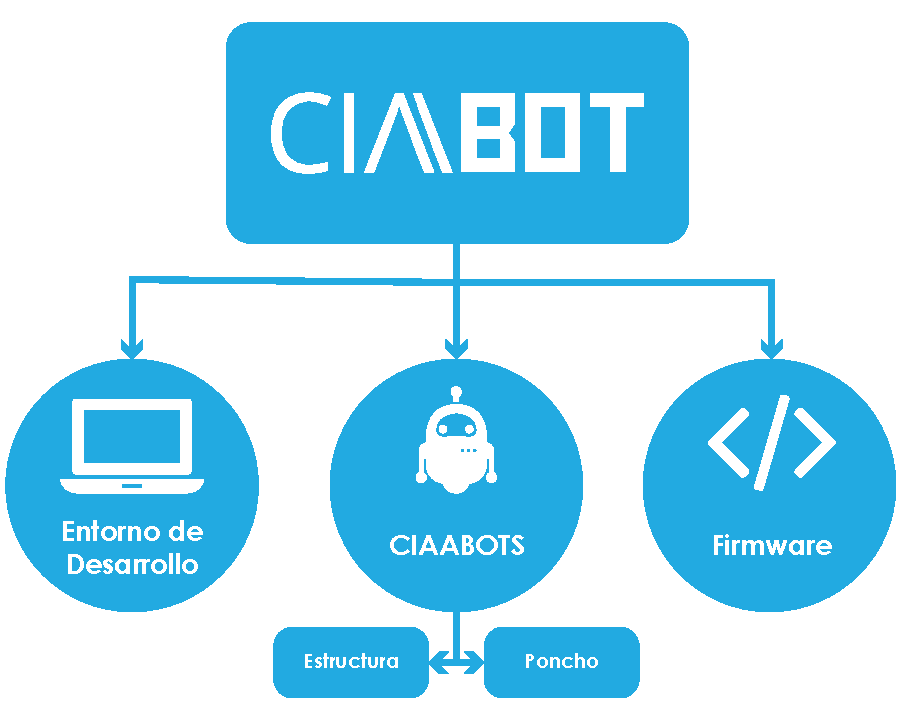
\includegraphics[scale=.8]{./Figures/ciaabot-partes.pdf}
    \label{fig:ciaabot:partes}
    \captionof{figure}{Diagrama de las partes que componen CIAABOT.}
\end{center}


\subsection{Entorno de desarrollo integrado}
\label{subsec:ide}
Un IDE (\emph{Integrated Development Environment}, Entorno de Desarrollo Integrado) es un software que incluye varias herramientas para asistir a los desarrolladores con su trabajo. Generalmente incluye algún editor para el código, herramientas de construcción o compilación automáticas, programación de la plataforma y posible depuración.

El CIAABOT-IDE es el centro del trabajo de los usuarios. Aquí plasman sus ideas y soluciones a problemas planteados. Esto lo hacen por medio de un editor de código en el que utilizan bloques predefinidos y no texto, como se observa en la figura \ref{fig:ciaabot:ide}. Arrastrando e interconectando los mismos logran definir la lógica para su programa.

Una opción interesante para remarcar es la salida de código en C. Cada vez que se modifica el diagrama de bloques, el código en C producido se modifica en tiempo real. Esto es muy útil para gente que pretende aprender a programar en C, ya que ve de manera directa cómo afecta cada bloque a las líneas de código y puede apreciar las equivalencias.

La plataforma también permite compilar y luego descargar el código generado en la placa solamente conectándola por USB.

Una vez que se finalizó el trabajo se puede guardar el proyecto en un archivo \emph{.cbp} que contiene la estructura de bloques en la que se estuvo trabajando, junto con las opciones adicionales del proyecto. Este archivo puede ser compartido y abierto en otra PC para ser reutilizado o modificado y guardado nuevamente.

Otra de las opciones que fue publicada en la última versión de CIAABOT-IDE (v0.0.8) es la de seleccionar los directorios de búsqueda para el toolchain. Las aplicaciones necesarias para todos los sistemas operativos son dos: El compilador arm-none-eabi-gcc y el debugger openOCD. Adicionalmente, en Windows se requieren otros ejecutables como make, para poder compilar y descargar el programa.

\begin{figure}[h]
	\centering
	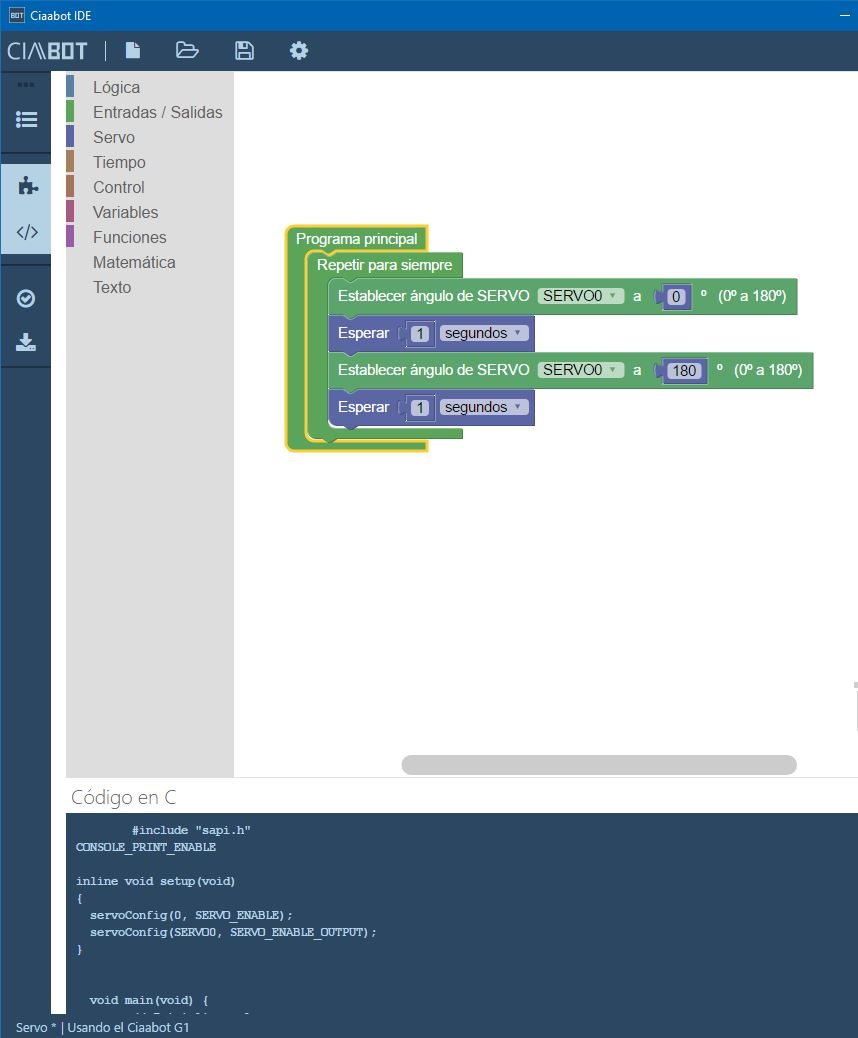
\includegraphics[scale=.5]{./Figures/ciaabot-ide-bloques.jpg}
	\caption{Editor gráfico de CIAABOT-IDE.}
	\label{fig:ciaabot:ide}
\end{figure}

\subsection{CIAABOTS}
\label{subsec:ciaabots}
Los robots que funcionen bajo esta plataforma serán denominados \emph{CIAABOTS}. Siguiendo la idea original de que CIAABOT sea utilizada en escuelas o por entusiastas, se planteó que estos robots estén diseñados estructuralmente para poder ser impresos con impresoras 3D.

De esta manera es posible enviar los archivos para imprimirlos en cualquier escuela que cuente con este sistema de impresión para replicarlo. Sólo sería necesario tener la placa CIAA correspondiente al modelo, armar el poncho (de diseño abierto) y adquirir en algún lugar de conveniencia los actuadores o sensores particulares del CIAABOT (motores DC, sensores IR, ultrasonido, etc.).

El diseño del poncho para el primer modelo de CIAABOT, el G1 se puede encontrar en github \citep{CIAABOT:G1}, realizado con el suite KiCad como todos los diseños relacionados al proyecto CIAA.

\subsection{Firmware}
\label{subsec:firmware}
CIAABOT utiliza como base para su firmware dos proyectos principales del ecosistema CIAA: Firmware v2 \citep{CIAA:firmwarev2} y sAPI \citep{sAPI}. En conjunto proveen una forma simplificada de programar las placas CIAA.

La sAPI es una HAL (\emph{Hardware Abstraction Layer}, Capa de Abstracción de Hardware) para los microcontroladores, que permite acceder de manera simple a varios de los diferentes periféricos.

Juntando varias funciones de la sAPI es posible armar funciones más complejas de mayor nivel para manejar características más específicas de cada modelo de CIAABOT.

Se prevé que con el avance del desarrollo de la plataforma cada modelo tendrá bloques específicos que estarán disponibles en el editor, cuando se lo seleccione a la hora de armar el proyecto en el IDE. Así, podrían armarse bloques que realicen por ejemplo una lectura de un sensor, que implicaría el manejo de pines y tiempos de espera.

\section{Plataforma utilizada}
\label{sec:plataforma}
Como base para el proyecto se optó por utilizar CIAA. Es un proyecto centrado en el trabajo colaborativo que busca la innovación para crear, diseñar y desarrollar soluciones electrónicas en la industria. Dentro de sus objetivos se encuentran:

\begin{itemize}
\item Impulsar el desarrollo tecnológico nacional, a partir de sumar valor agregado al trabajo y a los productos y servicios, mediante el uso de sistemas electrónicos, en el marco de la vinculación de las instituciones educativas y el sistema científico-tecnológico con la industria.

\item Darle visibilidad positiva a la electrónica argentina.

\item Generar cambios estructurales en la forma en la que se desarrollan y utilizan en nuestro país los conocimientos en el ámbito de la electrónica y de las instituciones y empresas que hacen uso de ella. \citep{CIAA:wiki}
\end{itemize}

Se utiliza esta plataforma por compartir la misma idea de ser un proyecto libre, poseer una creciente comunidad e incentivar la industria nacional. Se consideró que es un proyecto suficientemente maduro y con actualizaciones y desarrollos constantes como para ser utilizado de base.

\subsection{EDU-CIAA-NXP}
\label{subsec:eduCiaaNxp}
La EDU-CIAA-NXP es la versión educativa y de bajo costo de la CIAA-NXP. Utiliza, al igual que la CIAA-NXP, el microcontrolador LPC4337 de NXP, un doble núcleo ARM Cortex-M4F y Cortex M0. Como se observa en la figura \ref{fig:eduCiaaNxp}, la placa posee 4 leds y 4 pulsadores de hardware adicional. Para ampliar sus capacidades se utilizan los conectores laterales, para adicionar alguna placa extensora llamada \emph{Poncho}.

\begin{figure}[h]
\centering
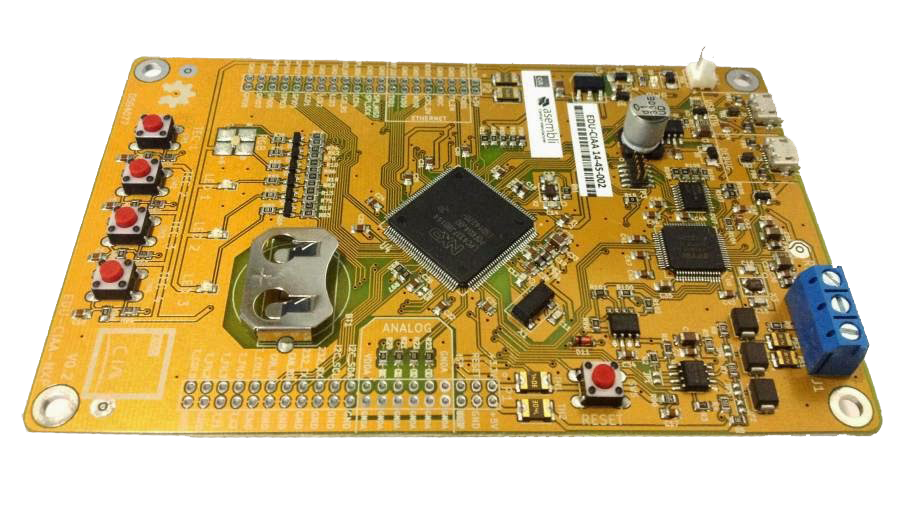
\includegraphics[scale=.5]{./Figures/edu-ciaa-nxp.png}
\caption{Placa EDU-CIAA-NXP}
\label{fig:eduCiaaNxp}
\end{figure}

Permite realizar programación y debugging, así como también acceder a una de sus UARTs, por medio de USB. Además posee otro puerto para que la placa funcione en modo OTG (\emph{On The Go}).

\section{Requerimientos}
\label{sec:requerimientos}
Se plantearon requerimientos que el proyecto debería cumplir a la hora de ser entregado. Se evaluaron sus posibilidades y se clasificaron en categorías.

\subsection{Requerimientos del sistema}
\label{subsec:requerimientosSistema}
Se estableció que el IDE debería poder ejecutarse como mínimo en un entorno Linux o Windows. Por la orientación didáctica del proyecto su uso debería ser simple, amigable y didáctico. Además, la programación debería poder realizarse íntegramente de manera gráfica por medio de bloques, donde cada uno represente acciones simples.

El IDE debería permitir un manejo de proyectos en forma de archivos, que posibilitaran el guardado y distribución de los mismos. Dentro de las opciones del proyecto debería poder seleccionarse el modelo de CIAABOT utilizado. Actualmente la opción existe, pero hay un solo modelo disponible.

El algoritmo que se genera a partir de los bloques debería estar disponible en lenguaje C, poder compilarse y programarse desde la aplicación, por puerto USB.

\subsection{Componentes del Sistema}
\label{subsec:componentesSistema}
Como ya se mencionó, se debería utilizar en principio la placa EDU-CIAA-NXP, y un poncho si fuese necesario para controlar la maqueta o robot implementado para la muestra. En el diseño de este poncho todos los periféricos deberían funcionar independientes al resto.

\subsection{Firmware}
\label{subsec:firmware}
Para el desarrollo del software se implementaría un sistema de control de versiones. Para la programación de los robots se utilizarían dos bibliotecas: En C la mencionada sAPI, y una de Firmata para un monitoreo del mismo por medio del puerto serie, con un cliente corriendo en la placa.

\subsection{Procesos Finales}
\label{subsec:procesosFinales}
Se requiere un manual de uso e instalación, junto con ejemplos básicos y funcionales, que sean representativos de las características de la plataforma. Se implementaría sobre una maqueta o robot adaptado a la EDU-CIAA, y con ello se evaluarían los resultados del proyecto y su aplicación en ámbitos de enseñanza reales.

\section{Planificación}
\label{sec:planificacion}
\subsection{Desglose en tareas}
En primer lugar, para definir objetivos concretos, se planteó una serie de entregables para el proyecto:

\begin{itemize}
\item IDE en funcionamiento.
\item Poncho CIAABOT G1 diseñado enteramente.
\item Manual de uso, instalación y ejemplos funcionales.
\item El presente informe final.
\end{itemize}

Siguiendo los lineamientos de las estrategias vistas en la materia Gestión de Proyectos, se procedió al diseño de una lista de desglose del trabajo en tareas. Se estimó un tiempo aproximado de 615 horas, distribuidas en grupos de tareas de la siguiente manera:

\begin{itemize}
\item Planificación del proyecto (40 hs.).
\item Investigación preliminar (45 hs.).
\item Selección de bibliotecas y plataformas (30 hs.).
\item Desarrollo de la aplicación de escritorio (45 hs.).
\item Desarrollo del editor gráfico (55 hs.).
\item Programación por USB y monitoreo (60 hs.).
\item Desarrollo del hardware (100 hs.).
\item Desarrollo del firmware (70 hs.).
\item Integración del sistema (50 hs.).
\item Procesos finales (120 hs.).
\end{itemize}
 
\chapter{Diseño e Implementación} % Main chapter title

\label{Chapter3} % Change X to a consecutive number; for referencing this chapter elsewhere, use \ref{ChapterX}
\definecolor{mygreen}{rgb}{0,0.6,0}
\definecolor{mygray}{rgb}{0.5,0.5,0.5}
\definecolor{mymauve}{rgb}{0.58,0,0.82}

\lstset{ %
  backgroundcolor=\color{white},   % choose the background color; you must add \usepackage{color} or \usepackage{xcolor}
  basicstyle=\footnotesize,        % the size of the fonts that are used for the code
  breakatwhitespace=false,         % sets if automatic breaks should only happen at whitespace
  breaklines=true,                 % sets automatic line breaking
  captionpos=b,                    % sets the caption-position to bottom
  commentstyle=\color{mygreen},    % comment style
  deletekeywords={...},            % if you want to delete keywords from the given language
  %escapeinside={\%*}{*)},          % if you want to add LaTeX within your code
  %extendedchars=true,              % lets you use non-ASCII characters; for 8-bits encodings only, does not work with UTF-8
  %frame=single,	                   % adds a frame around the code
  keepspaces=true,                 % keeps spaces in text, useful for keeping indentation of code (possibly needs columns=flexible)
  keywordstyle=\color{blue},       % keyword style
  language=[ANSI]C,					% the language of the code
  %otherkeywords={*,...},           % if you want to add more keywords to the set
  numbers=left,                    % where to put the line-numbers; possible values are (none, left, right)
  numbersep=5pt,                   % how far the line-numbers are from the code
  numberstyle=\tiny\color{mygray}, % the style that is used for the line-numbers
  rulecolor=\color{black},         % if not set, the frame-color may be changed on line-breaks within not-black text (e.g. comments (green here))
  showspaces=false,                % show spaces everywhere adding particular underscores; it overrides 'showstringspaces'
  showstringspaces=false,          % underline spaces within strings only
  showtabs=false,                  % show tabs within strings adding particular underscores
  stepnumber=1,                    % the step between two line-numbers. If it's 1, each line will be numbered
  stringstyle=\color{mymauve},     % string literal style
  tabsize=2,	                   % sets default tabsize to 2 spaces
  title=\lstname,                   % show the filename of files included with \lstinputlisting; also try caption instead of title
  morecomment=[s]{/*}{*/}%
}


%----------------------------------------------------------------------------------------
%	SECTION 1
%----------------------------------------------------------------------------------------
\section{Estructura del Software}

sAPI
\begin{itemize}
\item Interrupciones.
\item SysTick.
\item GPIO.
\item UART.
\item ADC.
\item DAC.
\item $I^2C$.
\item SPI.
\item RTC.
\item SCT.
\item Timers.
\end{itemize}

Además incluye funciones avanzadas de conversión de datos, impresión formateada por UART, manejo de displays 7 segmentos, teclados matriciales, servos y PWM entre otras.

%----------------------------------------------------------------------------------------
La idea de esta sección es resaltar los problemas encontrados, los criterios utilizados y la justificación de las decisiones que se hayan tomado.

Se puede agregar código o pseudocódigo dentro de un entorno lstlisting con el siguiente código:

\begin{verbatim}
\begin{lstlisting}[caption= "un epígrafe descriptivo"]

	las líneas de código irían aquí...
	
\end{lstlisting}
\end{verbatim}

A modo de ejemplo:

\begin{lstlisting}[caption=Pseudocódigo del lazo principal de control.]  % Start your code-block

#define MAX_SENSOR_NUMBER 3
#define MAX_ALARM_NUMBER  6
#define MAX_ACTUATOR_NUMBER 6

uint32_t sensorValue[MAX_SENSOR_NUMBER];		
FunctionalState alarmControl[MAX_ALARM_NUMBER];	//ENABLE or DISABLE
state_t alarmState[MAX_ALARM_NUMBER];						//ON or OFF
state_t actuatorState[MAX_ACTUATOR_NUMBER];			//ON or OFF

void vControl() {

	initGlobalVariables();
	
	period = 500 ms;
		
	while(1) {

		ticks = xTaskGetTickCount();
		
		updateSensors();
		
		updateAlarms();
		
		controlActuators();
		
		vTaskDelayUntil(&ticks, period);
	}
}
\end{lstlisting}




% Chapter Template

\chapter{Ensayos y Resultados} % Main chapter title

\label{Chapter4} % Change X to a consecutive number; for referencing this chapter elsewhere, use \ref{ChapterX}

%----------------------------------------------------------------------------------------
%	SECTION 1
%----------------------------------------------------------------------------------------

Este capítulo describe las pruebas que se realizaron sobre la plataforma, así como también su utilización en una situación aúlica real para dictado de cursos.

\section{Pruebas de sensores y actuadores}
\label{sec:pruebas}
Una vez desarrollados todos los bloques propuestos para la primera versión de la definición del lenguaje de CIAABOT, se pasó a una etapa de pruebas, para verificar que el manejo de los diferentes periféricos fuera correcta.

La primera prueba fue sobre un modelo impreso en 3D de un dedo índice, que es flexionado por un mecanismo accionado por un servomotor. En la figura \ref{fig:dedoServo} se observa el ensayo. Adicionalmente, la prueba también evaluó el funcionamiento de la lectura del conversor analógico-digital. Para esto se conectó un potenciómetro al canal 1 de conversión, que era leído constantemente.

El valor obtenido por el conversor (rango de 0 a 1023) era mapeado luego al rango admitido por la función de posicionamiento del servomotor (0 a 180), y luego era enviado al bloque de manejo del ángulo.

\begin{figure}[h]
\centering
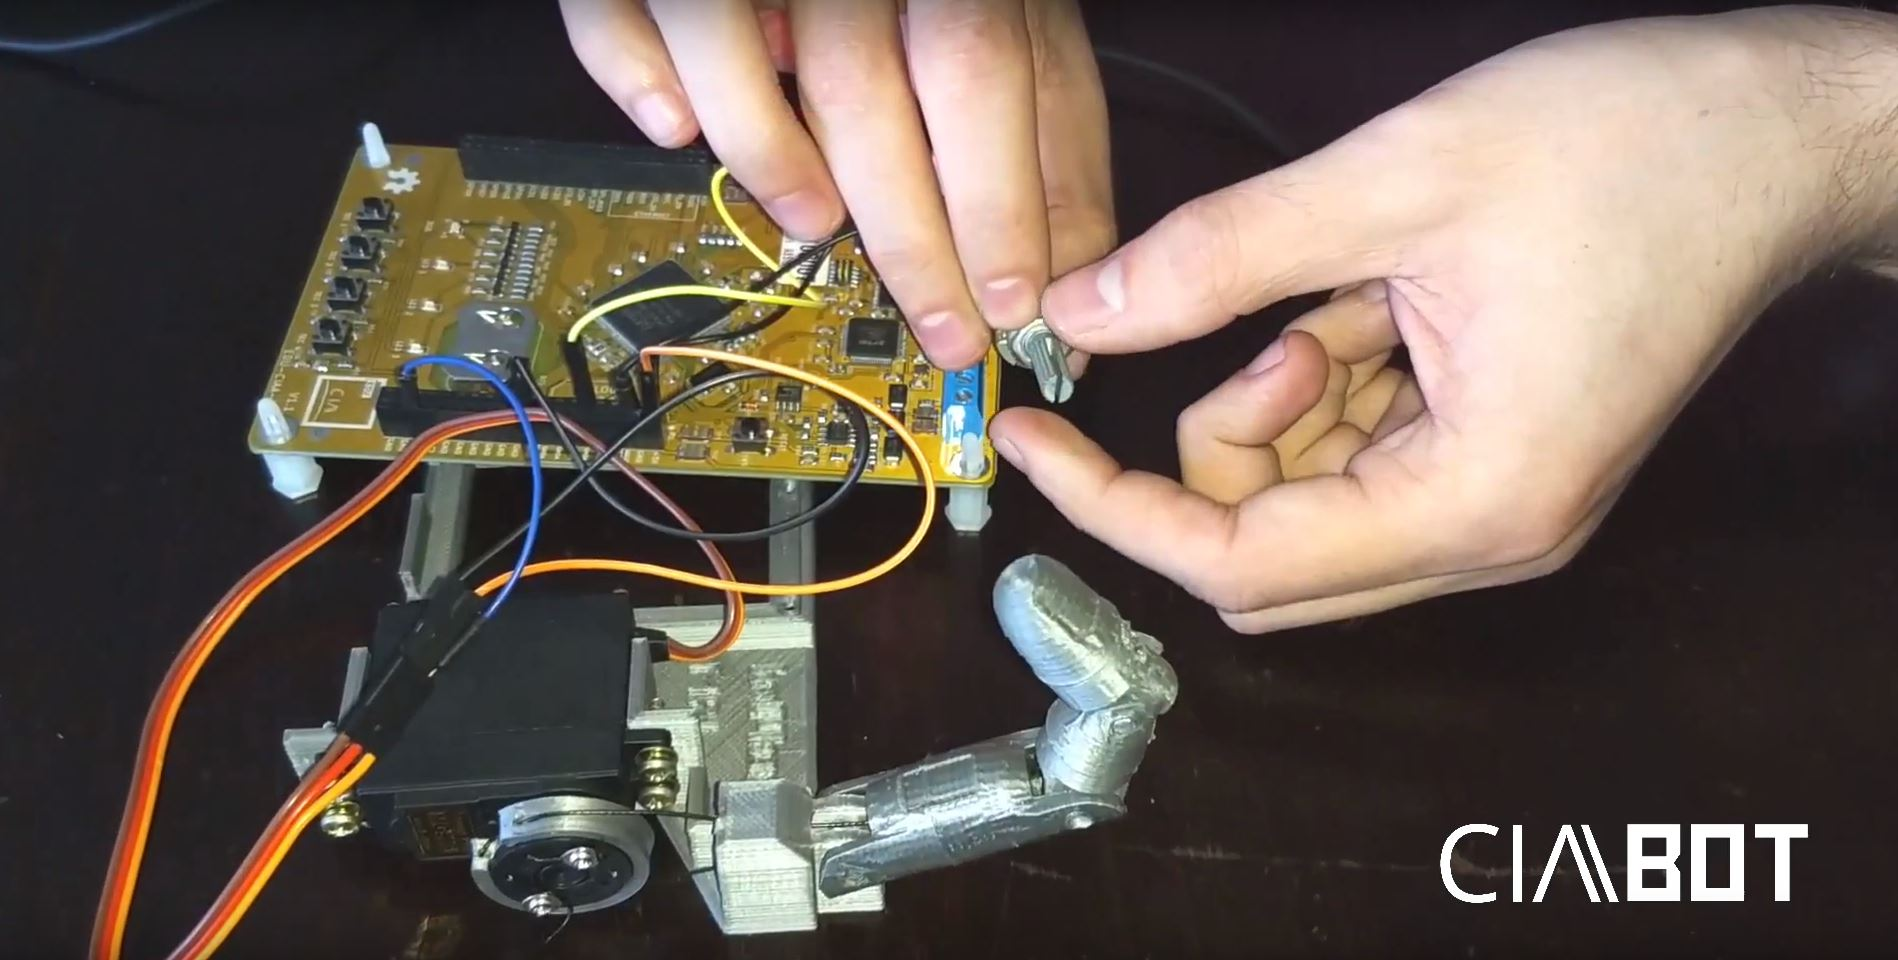
\includegraphics[scale=.3]{./Figures/dedo-servo.jpg}
\caption{Prueba de servomotor sobre dedo 3D.}
\label{fig:dedoServo}
\end{figure}

Teniendo en mente la necesidad de desarrollar ejemplos didácticos para utilizar CIAABOT, se utilizaron materiales desarrollados y provistos por la Universidad Nacional de Quilmes, en el marco del proyecto "La universidad y la escuela secundaria", dirigido por Cristina Wainmaier (Vicedirectora del Dto. de CyT, UNQ). Estos materiales incluían una maqueta de manejo de barreras y semáforos e instrumentos meteorológicos.

Para la verificación del correcto manejo del tiempo por parte del programa, se utilizó un anemómetro. Este dispositivo, que puede apreciarse en la figura \ref{fig:anemometro}, gira ante la presencia de viento y genera pulsos a intervalos angulares fijos. Conociendo la frecuencia de estos pulsos es posible determinar la velocidad del viento en cada momento.

Además, en este ensayo se probó la UART, proveyendo de una salida de consola por puerto serie, que podía observarse desde la PC. De esta manera el programa podía informar las mediciones realizadas, y guardarse en un archivo de log.

\begin{figure}[h]
\centering
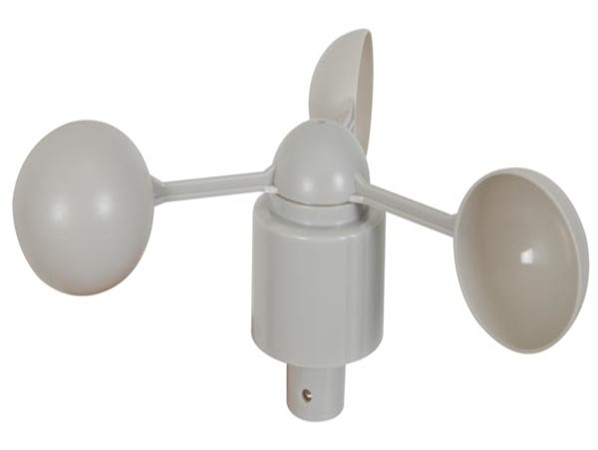
\includegraphics[scale=.8]{./Figures/anemometro.jpg}
\caption{Anemómetro utilizado en las pruebas.}
\label{fig:anemometro}
\end{figure}

De los instrumentos meteorológicos también se utilizó una rosa de los vientos formada por una matriz de leds. Con esto se validó el funcionamiento de las salidas digitales funcionando a la vez. En la figura \ref{fig:rosaVientos}, se observa un dibujo de la rosa de los vientos utilizada, así como la conexión de la matriz de leds que posee para encender los diferentes puntos cardinales.

\begin{figure}[H]
\centering
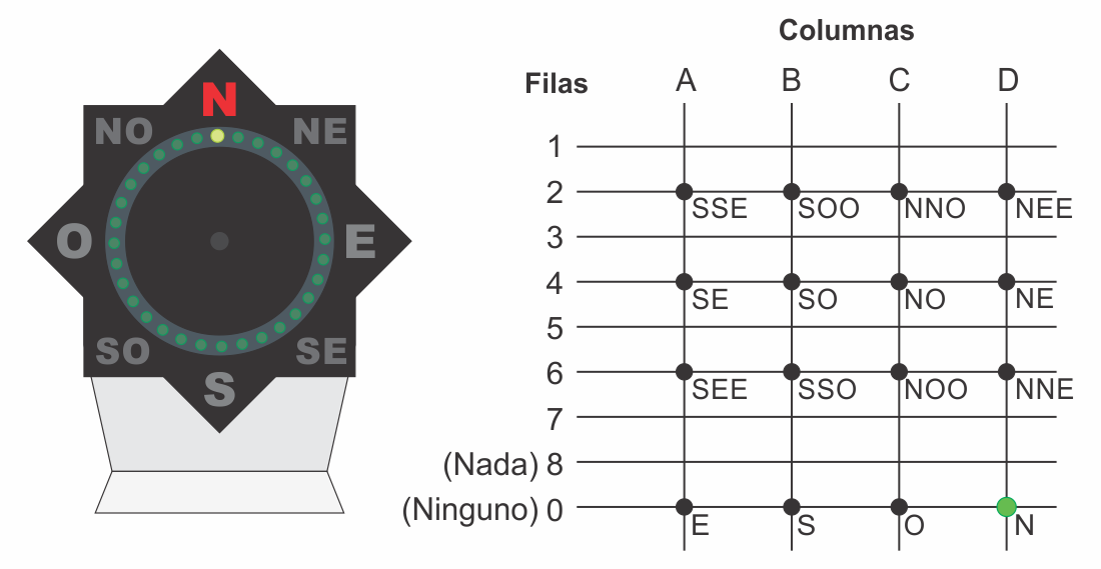
\includegraphics[scale=.6]{./Figures/rosa-vientos.png}
\caption{Rosa de los vientos y conexión de los leds.}
\label{fig:rosaVientos}
\end{figure}

\section{Workshop en el SASE}
Desde el 2010 se viene realizando año a año el Simposio Argentino de Sistemas Embebidos. Este evento es organizado por ACSE (Asociación Civil para la Investigación Promoción y Desarrollo de los Sistemas Electrónicos Embebidos). Es un evento anual que reúne a la comunidad académica y a la industria  en torno a esta temática, donde se realizan Tutoriales, Workshops y el Congreso Argentino de Sistemas Embebidos. 

En la edición de este año se agregó el workshop "Introducción a la programación de sistemas embebidos utilizando CIAABOT", que tuve la posibilidad de dictar y organizar en conjunto con el Ing. Eric Pernía. Estuvo orientado principalmente a alumnos de escuelas secundarias o entusiastas que buscaran una introducción a la programación de embebidos pero que no tuvieran conocimientos de ningún lenguaje para hacerlo.

Con una buena concurrencia se desarrolló la primera experiencia real en campo de la utilización de la plataforma CIAABOT para la enseñanza de programación. Se abarcaron temas básicos como el funcionamiento de sentencias condicionales, estructuras de control, lógica booleana y manejo básico de periféricos.

El workshop se realizó utilizando solamente CIAABOT IDE como medio para programar las placas. Se hizo uso de los elementos meteorológicos y la maqueta vehicular descrita en la sección \ref{sec:pruebas}, que puede observarse en la figura \ref{fig:maqueta}. Fue una buena oportunidad para obtener devoluciones por parte de los primeros usuarios de prueba, que fueron los asistentes al curso. Encontraron la aplicación intuitiva y se desenvolvieron de manera natural. Hubo dos casos puntuales de personas que no habían programado nunca antes de asistir, y ambos pudieron completar satisfactoriamente los ejercicios propuestos.

\begin{figure}[H]
\centering
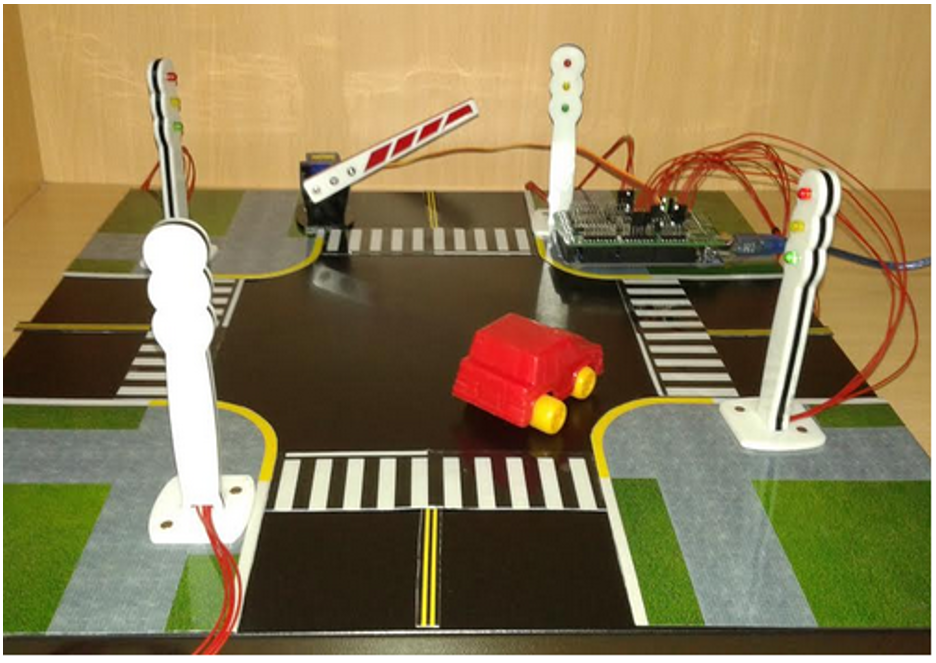
\includegraphics[scale=.8]{./Figures/maqueta.png}
\caption{Maqueta vehicular utilizada en el workshop.}
\label{fig:maqueta}
\end{figure}

\section{Experiencias en cursos CAPSE y de INET}
Los Cursos Abiertos de Programación de Sistemas Embebidos están orientados a personas con o sin experiencia previa, como docentes secundarios o universitarios, personal de empresas o estudiantes, que estén interesados en aprender a trabajar con sistemas embebidos. El objetivo de los cursos es aprender a realizar aplicaciones electrónicoas basadas en microcontroladores ARM de 32 bits, abordando desde problemas simples hasta problemas de mayor complejidad. Se utilizan kits compuestos por sensores y actuadores, y placas EDU-CIAA-NXP.

Además, cursos similares, y con objetivos alineados a los de los CAPSE, se brindaron a pedido del Instituto Nacional de Educación Tecnológica (INET).

En la última edición de estos cursos se utilizó CIAABOT IDE para las primeras clases, como manera de introducir a los asistentes a los conceptos básicos de la programación, así como también para obtener resultados rápidos. 

Esta segunda experiencia de uso de CIAABOT en un entorno real de enseñanza fue realmente útil. Se obtuvieron recomendaciones y se registraron errores descubiertos a raíz de casos de uso que no se tuvieron en cuenta a la hora del desarrollo. Todas estas mejoras y errores fueron registrados en la sección de \emph{issues} del repositorio de CIAABOT.

Por ejemplo, gran parte de los asistentes poseían netbooks con pantallas de resolución limitada, lo que hacía algo dificultoso el manejo de la vista partida que presenta el editor gráfico del IDE en conjunto con la salida del código C. Además, la sección de proyectos recientes y el formulario de 'Nuevo Proyecto' no se mostraban de manera cómoda. A raíz de esto, se comenzó un proceso de mejora de la adaptación de la aplicación ante cambios de resoluciones de pantalla, a lo que se refiere en inglés como  \emph{responsiveness}.

\section{Uso en un proyecto de brazo robótico}
El Laboratorio Abierto de la Universidad Tecnológica Nacional Facultad Regional Avellaneda, comenzó este año el desarrollo de una prótesis de brazo y mano robótica, impresas en 3D. La mano cuenta con movilidad en la muñeca y las falanges de los dedos, logrando así una funcionalidad similar a la de la mano humana. El brazo puede observarse en la figura \ref{fig:brazo}.

\begin{figure}[H]
\centering
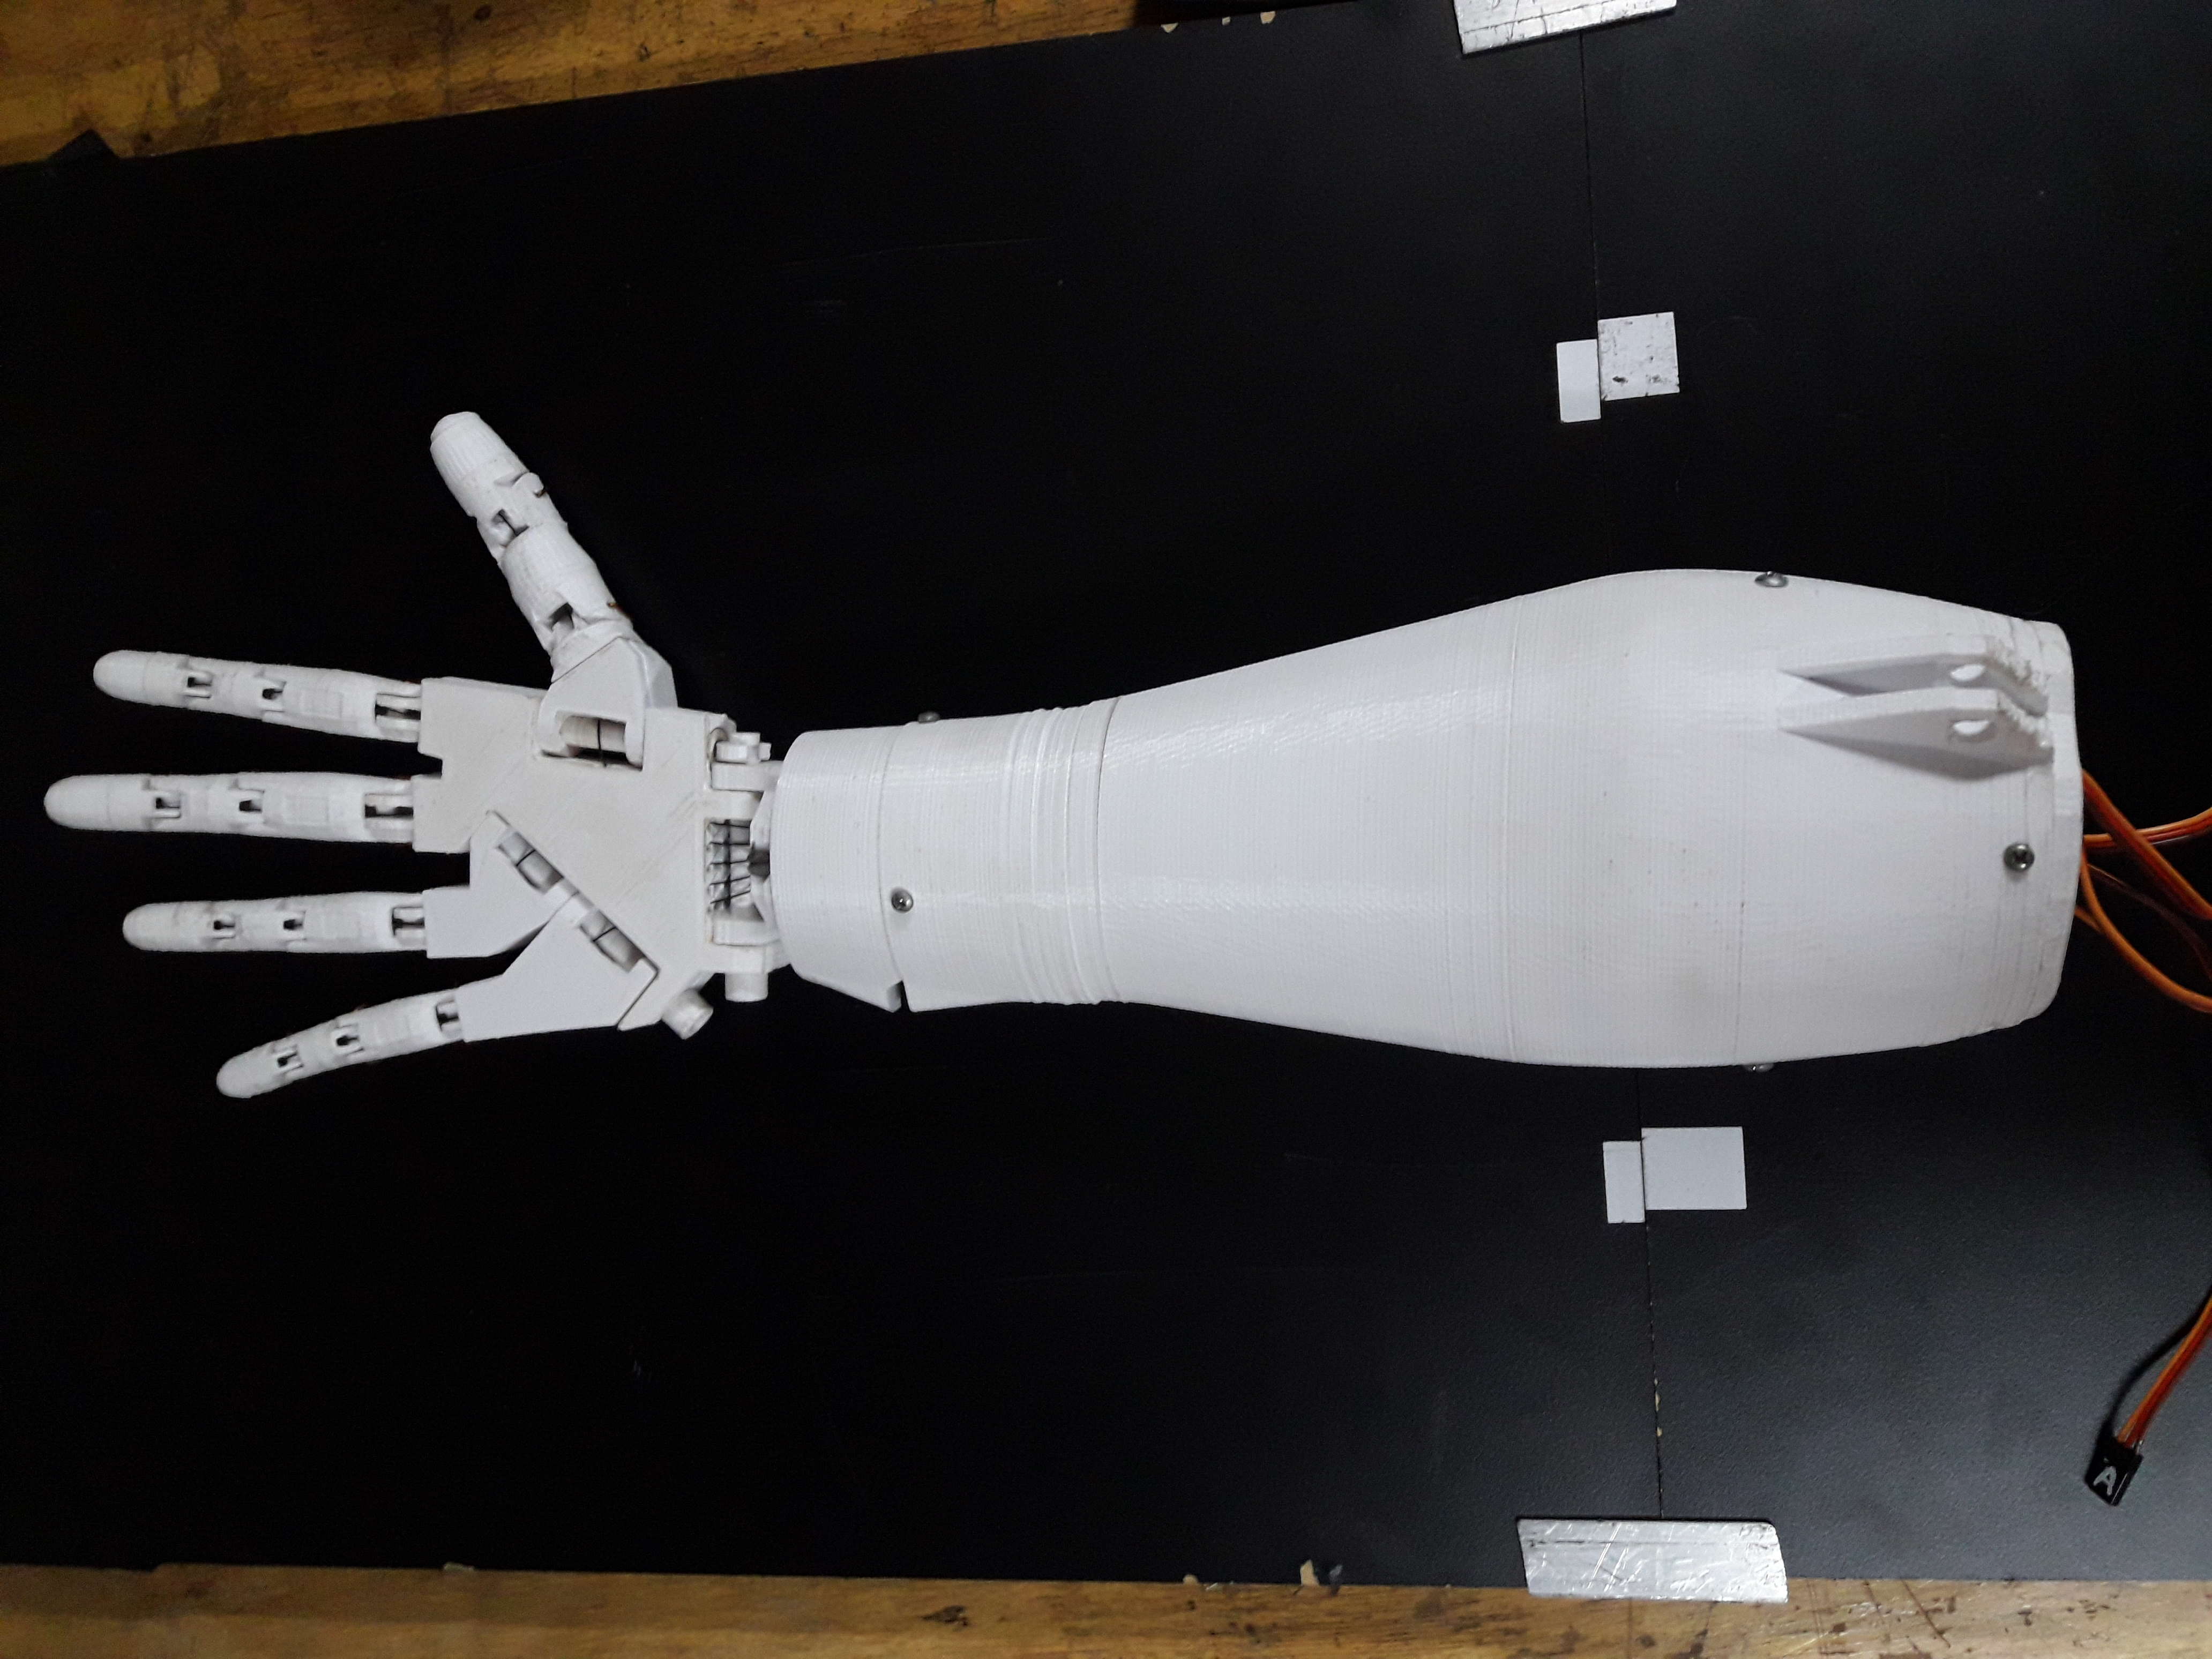
\includegraphics[scale=.1]{./Figures/brazo.jpg}
\caption{Prótesis impresa en 3D.}
\label{fig:brazo}
\end{figure}

El objetivo principal del mismo, es poder realizar un aporte a la mejora de la calidad de vida de personas con amputaciones parciales de brazo y mano. Se utilizan las señales bioeléctricas obtenidas superficialmente desde el músculo del usuario para luego transformarla en una señal eléctrica capaz de manipularse, con el fin de controlarla. Por tal motivo, el faltante de miembro del paciente no debe ser total, para permitir una colocación de 3 electrodos.

Actualmente el proyecto busca migrarse a microcontroladores de 32 bits, y se optó utilizar la placa EDU-CIAA-NXP. Esto es debido a que las mediciones de los electrodos sirven para realizar un control rudimentario y detectar si el músculo está contraído o no, pero no alcanza para obtener una señal proporcional a la fuerza ejercida para emular este movimiento en la prótesis.

La idea es mejorar algoritmo de detección de fuerza en el músculo, realizando un análisis en el dominio de la frecuencia con el objetivo de eliminar ruidos propios que se generan por el tipo de contacto que tienen los sensores. Para esto, se pretende hacer uso de la unidad de punto flotante presente en el LPC4337. Para las primeras pruebas de manejo de hardware y lectura de los sensores musculares, se utilizaron programas armados en CIAABOT IDE.
 
% Chapter Template

\chapter{Conclusiones} % Main chapter title

\label{Chapter5} % Change X to a consecutive number; for referencing this chapter elsewhere, use \ref{ChapterX}


%----------------------------------------------------------------------------------------

%----------------------------------------------------------------------------------------
%	SECTION 1
%----------------------------------------------------------------------------------------

\section{Conclusiones generales }

La idea de esta sección es resaltar cuáles son los principales aportes del trabajo realizado y cómo se podría continuar. Debe ser especialmente breve y concisa. Es buena idea usar un listado para enumerar los logros obtenidos.

%----------------------------------------------------------------------------------------
%	SECTION 2
%----------------------------------------------------------------------------------------
\section{Próximos pasos}

Acá se indica cómo se podría continuar el trabajo más adelante.
 

%----------------------------------------------------------------------------------------
%	CONTENIDO DE LA MEMORIA  - APÉNDICES
%----------------------------------------------------------------------------------------

\appendix % indicativo para indicarle a LaTeX los siguientes "capítulos" son apéndices

% Incluir los apéndices de la memoria como archivos separadas desde la carpeta Appendices
% Descomentar las líneas a medida que se escriben los apéndices

%% Appendix A

\chapter{Appendix Title Here} % Main appendix title

\label{AppendixA} % For referencing this appendix elsewhere, use \ref{AppendixA}

Write your Appendix content here.
%\include{Appendices/AppendixB}
%\include{Appendices/AppendixC}

%----------------------------------------------------------------------------------------
%	BIBLIOGRAPHY
%----------------------------------------------------------------------------------------

\Urlmuskip=0mu plus 1mu\relax
\raggedright
\printbibliography[heading=bibintoc]

%----------------------------------------------------------------------------------------

\end{document}  
